%----------------------------------------------
%	PACKAGES AND OTHER DOCUMENT CONFIGURATIONS
%----------------------------------------------
\documentclass[11pt, a4paper, oneside]{Thesis} % Paper size, default font size and one-sided paper

\graphicspath{{./Pictures/}} % Specifies the directory where pictures are stored

%\usepackage{cite}
\usepackage[square, numbers, comma, sort&compress]{natbib} % Use the natbib reference package - read up on this to edit the reference style; if you want text (e.g. Smith et al., 2012) for the in-text references (instead of numbers), remove 'numbers' 
\hypersetup{urlcolor=blue, colorlinks=true} % Colors hyperlinks in blue - change to black if annoying
\title{\ttitle} % Defines the thesis title - don't touch this

\begin{document}

\frontmatter % Use roman page numbering style (i, ii, iii, iv...) for the pre-content pages

\setstretch{1.3} % Line spacing of 1.3

% Define the page headers using the FancyHdr package and set up for one-sided printing
\fancyhead{} % Clears all page headers and footers
\rhead{\thepage} % Sets the right side header to show the page number
\lhead{} % Clears the left side page header

\pagestyle{fancy} % Finally, use the "fancy" page style to implement the FancyHdr headers

\newcommand{\HRule}{\rule{\linewidth}{0.5mm}} % New command to make the lines in the title page

% PDF meta-data
\hypersetup{pdftitle={\ttitle}}
\hypersetup{pdfsubject=\subjectname}
\hypersetup{pdfauthor=\authornames}
\hypersetup{pdfkeywords=\keywordnames}

%-----------------
%	TITLE PAGE
%---------------

\begin{titlepage}
\begin{center}

\textsc{\Large \univname}\\[1cm] % University name

\HRule \\[0.4cm] % Horizontal line
{\huge \bfseries \ttitle}\\[0.4cm] % Thesis title
\HRule \\[1.5cm] % Horizontal line
 
\begin{minipage}{0.4\textwidth}
\begin{flushleft} \large
\emph{Authors:}\\
\authornames % Author name - add \href bracket with link to add a website
\end{flushleft}
\end{minipage}
\begin{minipage}{0.4\textwidth}
\begin{flushright} \large
\emph{Supervisor:} \\
\supname % Supervisor name - add \href bracket with link to add a website
\end{flushright}
\end{minipage}\\[11cm]
\groupname\\
 
{\large November 2013}\\[1cm] % Date

\begin{tabular}{lr}
   
\includegraphics[scale=0.6]{./Figures/NTNU-logo.pdf} 
   \hspace{3 cm} &
   
\includegraphics[scale=0.9]{./Figures/HDIR-LOGO-HORISONTAL-ENG-CMYK.pdf} \\
\end{tabular}
\end{center}
\end{titlepage}
\clearpage % Start a new page

%---------------
%	ABSTRACT PAGE
%----------------

\addtotoc{Abstract} % Add the "Abstract" page entry to the Contents

\abstract{\addtocontents{toc}{\vspace{1em}}
This report describes the design of the National Integration Platform (NIP) used for Citizen Centric eHealth in Norway. 
The NIP is a platform to collect different user generated eHealth data from third party solutions and services. 
It also describes the making of the working prototype. 
The challenges of this prototype is to demonstrate the transfer of personal and/or medical data from different devices and systems.
The intention of the platform is to enable citizens the ability to publish information they produce into the government run NIP. 
It is worth noting that security is not a requirement of the prototype.
To demonstrate these different parts the creation of an Android application (App), a web App and a back-end Application Programming Interface (API) was required. 

The motivation for working in this project is to innovate and create a new platform that can be used to better understand the health of citizens. 
The citizens gather various health data from different locations and devices and in return provide a better understanding of the citizens health. 
Together with educated health professionals and doctors this can be a powerful tool for improving the quality of life of the users. 
The most interesting part was to figure out how to design a system that can have the high level of security required to transfer personal health information. 

The demands were to plan, design and describe the NIP and to develop a prototype. 
The demonstration of this product is aimed mainly at two groups of people: \\
1. Educated health professionals \\
2. Developers \\
The product should have a demonstration side that is easy for the first group to grasp, understand and form an idea of how it will work while also making it appealing and technical for the second group. 

The result of this project is first and foremost a working prototype of a NIP. 
It is also a web App and an Android app to make the demonstration easier to grasp. 
This report is also part of the result which has the purpose of documenting the problem, the process, the workflow and the final products.
}
\clearpage % Start a new page

%------------------
%	PreFace
%------------------

\addtotoc{Preface} 

\preface{\addtocontents{toc}{\vspace{1em}}
This report is for the main project in the course TDT4290 Customer Driven Project at NTNU. The project was executed on behalf of Helsedirektoratet or The Norwegian Directorate of Health. The team consisted of three students from NTNU. 

The team would like to thank our supervisor Meng Zhu for his guidence, help and advice for this project. 

In addition we would also like to thank our customer Helsedirektoratet and their contact person Helge T. Blindheim for their effort. 

%Thank the people from usability/design tests valuable feedback?
}
\clearpage % Start a new page

%-----------------------------------------
%	LIST OF CONTENTS/FIGURES/TABLES PAGES
%------------------------------------------

\pagestyle{fancy} % The page style headers have been "empty" all this time, now use the "fancy" headers as defined before to bring them back

\lhead{\emph{Contents}} % Set the left side page header to "Contents"
\tableofcontents % Write out the Table of Contents

\lhead{\emph{List of Figures}} % Set the left side page header to "List of Figures"
\listoffigures % Write out the List of Figures

\lhead{\emph{List of Tables}} % Set the left side page header to "List of Tables"
\listoftables % Write out the List of Tables

%----------------
%	ABBREVIATIONS
%-------------------

\clearpage % Start a new page

\setstretch{1.5} % Set the line spacing to 1.5, this makes the following tables easier to read

\lhead{\emph{Abbreviations}} % Set the left side page header to "Abbreviations"
\listofsymbols{ll} % Include a list of Abbreviations (a table of two columns)
{
\textbf{AJAX} & \textbf{A}synchronous \textbf{Ja}vaScript and \textbf{X}ML \\
\textbf{API} & \textbf{A}pplication \textbf{P}rogramming \textbf{I}nterface \\
\textbf{App} & \textbf{A}pplication \\
\textbf{CSS} & \textbf{C}ascading \textbf{S}tyle \textbf{S}heets \\
\textbf{DOM} & \textbf{D}ocument \textbf{O}bject \textbf{M}odel \\
\textbf{HTML} & \textbf{H}yper\textbf{T}ext \textbf{M}arkup \textbf{L}anguage \\
\textbf{IDI} & \textbf{I}nstitutt for \textbf{D}atateknikk og \textbf{I}nformasjonsvitenskap  \\
\textbf{JSP} & \textbf{J}ava\textbf{S}erver \textbf{P}ages \\
% Should we include the english name? Department of Computer and Information Science \\
\textbf{NIP} & \textbf{N}ational \textbf{I}ntegration \textbf{P}latform \\
\textbf{NTNU} & \textbf{N}orges \textbf{T}eknisk-\textbf{N}aturvitenskalige \textbf{U}niversitet \\
% Should we include the english name? \\Norwegian University of Science and Technology\\
\textbf{POM} & \textbf{P}roject \textbf{O}bject \textbf{M}odel \\
\textbf{SDK} & \textbf{S}oftware \textbf{D}evelopment \textbf{K}it \\
}

%-----------------------------
%	THESIS CONTENT - CHAPTERS
%------------------------------

\mainmatter % Begin numeric (1,2,3...) page numbering

\pagestyle{fancy} % Return the page headers back to the "fancy" style

% Include the chapters of the thesis as separate files from the Chapters folder
% Uncomment the lines as you write the chapters

% Chapter 1

\chapter{Introduction} % Main chapter title

\label{Introduction} % For referencing the chapter elsewhere, use \ref{Chapter1} 

\lhead{Chapter 1. \emph{Introduction}} % This is for the header on each page - perhaps a shortened title

%----------------------------------------------------------------------------------------

\section{Project description}

%----------------------------------------------------------------------------------------

\section{The client}
helsedirektoratet

\section{Involved parties}

Us and the supervisor.
two tables would look neat


%----------------------------------------------------------------------------------------

\section{Problem domain}
some text

\section{Project drivers}
people 

\section{Available resources}
\section{Limitations}
\section{Duration}
%% Chapter Template

\chapter{Project directive} % Main chapter title

\label{Chapter2} % Change X to a consecutive number; for referencing this chapter elsewhere, use \ref{ChapterX}

\lhead{Chapter 2. \emph{Project directive}} % Change X to a consecutive number; this is for the header on each page - perhaps a shortened title

%----------------------------------------------------------------------------------------
%	SECTION 1
%----------------------------------------------------------------------------------------

\section{Main Section 1}

Lorem ipsum dolor sit amet, consectetur adipiscing elit. Aliquam ultricies lacinia euismod. Nam tempus risus in dolor rhoncus in interdum enim tincidunt. Donec vel nunc neque. In condimentum ullamcorper quam non consequat. Fusce sagittis tempor feugiat. Fusce magna erat, molestie eu convallis ut, tempus sed arcu. Quisque molestie, ante a tincidunt ullamcorper, sapien enim dignissim lacus, in semper nibh erat lobortis purus. Integer dapibus ligula ac risus convallis pellentesque.

%-----------------------------------
%	SUBSECTION 1
%-----------------------------------
\subsection{Subsection 1}

Nunc posuere quam at lectus tristique eu ultrices augue venenatis. Vestibulum ante ipsum primis in faucibus orci luctus et ultrices posuere cubilia Curae; Aliquam erat volutpat. Vivamus sodales tortor eget quam adipiscing in vulputate ante ullamcorper. Sed eros ante, lacinia et sollicitudin et, aliquam sit amet augue. In hac habitasse platea dictumst.

%-----------------------------------
%	SUBSECTION 2
%-----------------------------------

\subsection{Subsection 2}
Morbi rutrum odio eget arcu adipiscing sodales. Aenean et purus a est pulvinar pellentesque. Cras in elit neque, quis varius elit. Phasellus fringilla, nibh eu tempus venenatis, dolor elit posuere quam, quis adipiscing urna leo nec orci. Sed nec nulla auctor odio aliquet consequat. Ut nec nulla in ante ullamcorper aliquam at sed dolor. Phasellus fermentum magna in augue gravida cursus. Cras sed pretium lorem. Pellentesque eget ornare odio. Proin accumsan, massa viverra cursus pharetra, ipsum nisi lobortis velit, a malesuada dolor lorem eu neque.

%----------------------------------------------------------------------------------------
%	SECTION 2
%----------------------------------------------------------------------------------------

\section{Main Section 2}

Sed ullamcorper quam eu nisl interdum at interdum enim egestas. Aliquam placerat justo sed lectus lobortis ut porta nisl porttitor. Vestibulum mi dolor, lacinia molestie gravida at, tempus vitae ligula. Donec eget quam sapien, in viverra eros. Donec pellentesque justo a massa fringilla non vestibulum metus vestibulum. Vestibulum in orci quis felis tempor lacinia. Vivamus ornare ultrices facilisis. Ut hendrerit volutpat vulputate. Morbi condimentum venenatis augue, id porta ipsum vulputate in. Curabitur luctus tempus justo. Vestibulum risus lectus, adipiscing nec condimentum quis, condimentum nec nisl. Aliquam dictum sagittis velit sed iaculis. Morbi tristique augue sit amet nulla pulvinar id facilisis ligula mollis. Nam elit libero, tincidunt ut aliquam at, molestie in quam. Aenean rhoncus vehicula hendrerit. 
\chapter{Project management}

\label{ch:management}
\lhead{Chapter 2. \emph{Project management}}
\nocite{Sommerville9}

This chapter covers project management topics such as planning, organization, risk management,
management rules and tools selection.

\section{Project planning}
\label{section:planning}
This section describes the planning of the project including its schedule and resources.

\subsection{Schedule}
\label{section:schedule}

\textbf{Milestones} \newline
We have identified four milestones for the project. These are associated with important events in the project lifetime
and can help us to better monitor its progress. Project's milestones are shown in table \ref{table:milestones}.

\begin{table}[h]
\begin{center}
\begin{tabular}{ | l | l | l | }
  \hline
  Milestone & Date & Description \\
  \hline\noalign{\smallskip}\hline
  M1 & 20.09.2013 & Basic implementation of the product. \\
                    %%\footnote{Consting of a backend, a frontend and one Android application}\\ 
  M2 & 14.10.2013 & Mid-term report delivery. \\
  M3 & 04.11.2013 & Feature freeze. \\
  M4 & 21.11.2013 & Project demonstration and final report delivery. \\
  \hline
\end{tabular}
\end{center}
\caption{Project milestones}
\label{table:milestones}
\end{table}

\textbf{Sprints schedule} \newline
Table \ref{table:sprints} contains an overview of the Sprints in the project.
Each sprint is described in a separate chapter.

\begin{table}[h]
\begin{center}
\begin{tabular}{ | l | l | l | }
  \hline
  Sprint & Start date & End date \\
  \hline\noalign{\smallskip}\hline
  0 & 26.08.2013 & 08.09.2013 \\ 
  1 & 09.09.2013 & 22.09.2013 \\
  2 & 23.09.2013 & 06.10.2013 \\
  3 & 07.09.2013 & 20.10.2013 \\
  4 & 21.10.2013 & 04.11.2013 \\
  5 & 05.11.2013 & 21.11.2013 \\
  \hline
\end{tabular}
\end{center}
\caption{Planned sprints}
\label{table:sprints}
\end{table}

%---

\subsection{Work plan}
\label{section:workplan}

The project work plan is shown in figure \ref{figure:work-plan}.
Project's phases can bee seen in figure \ref{figure:phase-plan}.

\newpage

\begin{landscape}
\begin{figure}
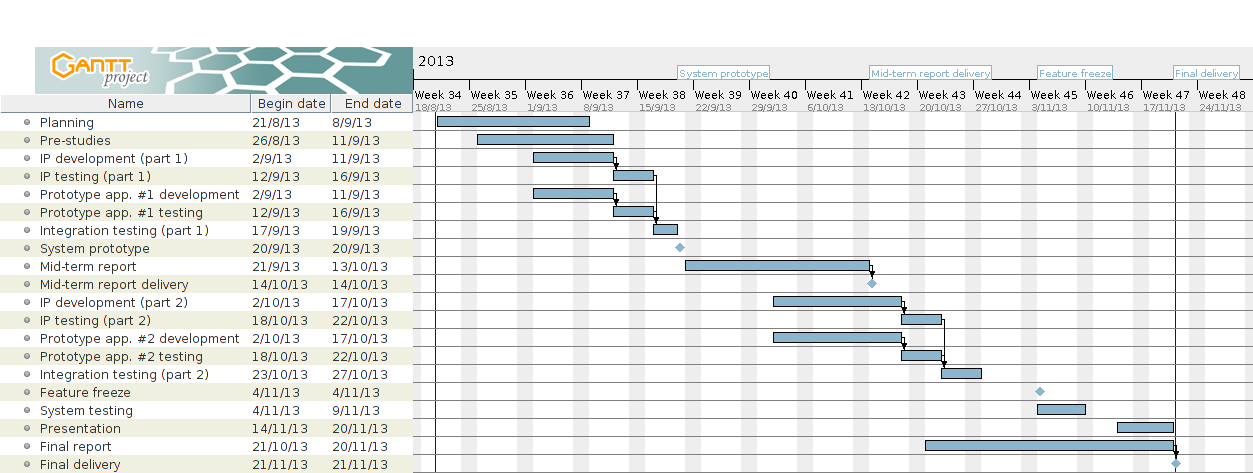
\includegraphics[scale=0.5]{../Figures/gantt-diagram.png}
\caption{Gantt diagram}
\label{figure:work-plan}
\end{figure}

\begin{figure}
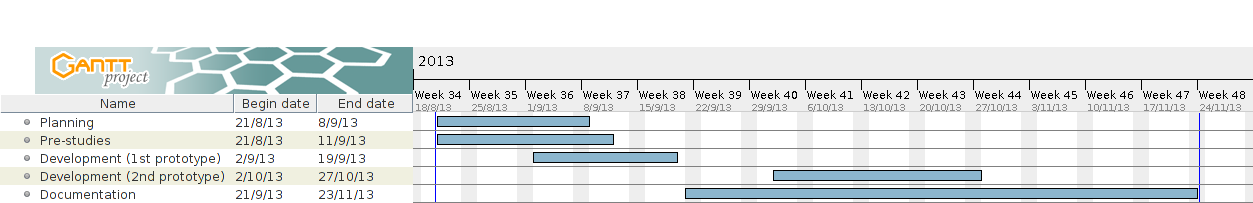
\includegraphics[scale=0.5]{../Figures/phases-diagram.png}
\caption{Phases diagram}
\label{figure:phase-plan}
\end{figure}

\end{landscape}

%---

\subsection{Resources}
\label{section:resources}
The team consists of three members from different educational backgrounds and with different skills.
In order to better distribute the work among us, we created a skill matrix regarding the technologies involved
in the project. The skills are valued on a scale of zero to five based on criteria detailed in table
\ref{table:skillscale}. Each value corresponds to a certain degree of proficiency, as described in table
\ref{table:proficiency}. The skill matrix is shown in table \ref{table:skillmatrix}.

\begin{table}[h]
\begin{center}
\begin{tabular}{ | c | l | l | }
  \hline
  Level & Proficiency & Criteria \\
  \hline\noalign{\smallskip}\hline
  0 & None		& Has no clue what we're talking about. \\
  1 & Basic		& Has read about it.\\
  2 & Fair		& Has studied it at school.\\
  3 & Good		& Personal interest, use in small-medium sized projects.\\
  4 & Very good	& Strong personal interest, use in medium-large sized projects. \\
  5 & Excellent	& 5+ Years of work experience. \\
  \hline
\end{tabular}
\end{center}
\caption{Skill's scale explanation}
\label{table:skillscale}
\end{table}

\begin{table}[h]
\begin{center}
\begin{tabular}{ | c | l | l | }
  \hline
  Level & Proficiency & Description \\
  \hline\noalign{\smallskip}\hline
  0 & None		  & Cannot perform the task \\
  1 & Basic     & Can perform the task with some help from other people \\
  2 & Fair		  & Can perform the task almost independently \\
  3 & Good		  & Can perform the task without any help \\
  4 & Very good	& Can help others to complete the task \\
  5 & Excellent	& Can help others to complete the task \\
  \hline
\end{tabular}
\end{center}
\caption{Proficiency level description}
\label{table:proficiency}
\end{table}

\begin{table}[h]
\begin{center}
\begin{tabular}{ | l | c | c | c | c | c | c | c | c | }
  \hline
  Team member & Java & JS & Android & Database & CSS & jQuery & Spring & LaTeX \\
  \hline\noalign{\smallskip}\hline
  Anders & 4 & 4 & 3 & 4 & 4 & 2 & 3 & 1 \\
  Emanuele & 4 & 1 & 3 & 2 & 1 & 1 & 0 & 3 \\
  Sebastian & 4 & 4 & 2 & 4 & 3 & 4 & 0 & 3 \\
  \hline
\end{tabular}
\end{center}
\caption{Skill matrix}
\label{table:skillmatrix}
\end{table}

%---
\newpage
\section{Project organization}
\label{section:organization}

This section covers the organizational aspects of the project such as roles description and allocation,
meetings schedule and specific group dynamics.

\subsection{Role description}
We have identified a number of roles in this project. Although each role has different, distinct responsibilities,
we see all roles as equally important for the success of this project.

\begin{description}
\iffalse
\item[Project manager]
%supposedly, there is no project manager in scrum !!
The project manager has the responsibility of managing the project.
This includes people management, high level project planning and risk analysis.
The project manager is also responsible of producing weekly status reports and communication with the
customer and supervisor.
\fi
\item[Scrum master]
The scrum master had the responsibility of helping team members perform Scrum.
Additionally, he was responsible of communication with both the customer and supervisor
and to produce status reports.
\item[Product owner]
The product owner was responsible of approving and prioritizing product's
requirements in order to steer its development in the direction he pleased.
\item[Secretary]
Responsible for taking notes during meetings and booking rooms.
\item[Quality assurance]
Ensured that quality practices were in place and use.
\item[Web developer]
Responsible for web development. Oversaw and took initiative on web development (front-end).
\item[Droid developer]
Responsible for Android development. Oversaw and took initiative on Android application development.
\item[System developer]
Responsible for developing the Spring backend, including database coding. Took care of system deployment.
%\item[System architect]
\end{description}

\subsection{Role allocation}

\begin{figure}[H]
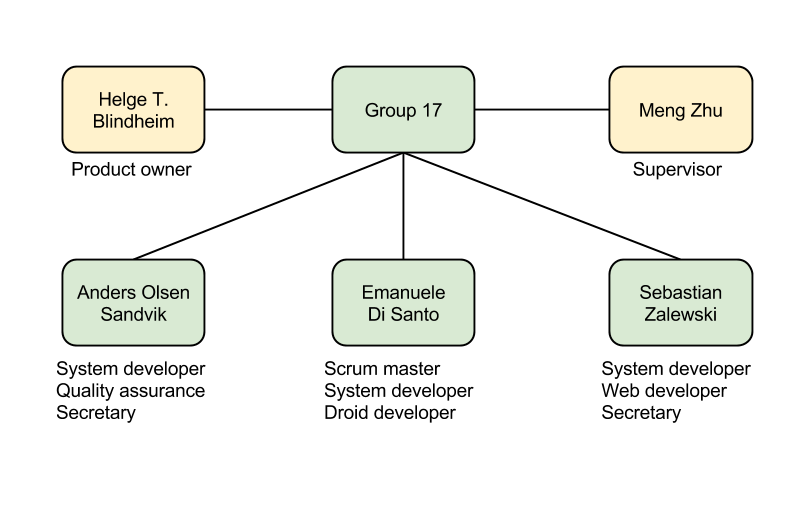
\includegraphics[scale=0.5]{../Figures/organizational-diagram.png}
\caption{Organizational diagram}
\label{figure:orgdia}
\end{figure}

Roles were allocated primarily on team members' competences.
Those roles that were left unassigned were taken up by members who volunteered upon approval 
of other team members. Because we were only three people, all of us had more than one role. Sometimes, roles were shared.
We tried to balance roles evenly between ourselves and achieve a flat group organization where no member
had a prominent role on others. Table \ref{table:roles} shows roles allocation within the group.
See figure \ref{figure:orgdia} for a diagram of how the group was organized.

\begin{table}[h]
\begin{center}
\begin{tabular}{ | l | l | }
  \hline
  \textbf{Member} & \textbf{Roles} \\
  \hline\noalign{\smallskip}\hline
  Anders Olsen Sandvik  &  System developer, Secretary, Quality assurance\\
  Emanuele Di Santo     &  Project manager, Droid developer, System developer\\
  Sebastian Zalewski    &  Web developer, System developer, Secretary\\
  \hline
\end{tabular}
\end{center}
\caption{Members' roles}
\label{table:roles}
\end{table}

\newpage
\section{Management rules}
\label{section:rules}

In this section we present our management rules and practices.

\subsection{Quality of the documentation}
Each document should be reviewed by another person other than the writer.
Especially for the report, we took care of reviewing each other's work in order to ensure
consistency and correctness throughout the document.

\subsection{Templates}
We have established templates for the following:
\begin{enumerate}
\item status reports
\item meeting notes for all meetings
\item meeting agendas for supervisor meetings
\end{enumerate}

Templates can be found in appendix \ref{AppendixC}.

\iffalse
\subsection{Standards}

\textbf{Coding style}
The adopted a camel case notation  for function and variables in Java

database, comments, function, brackets..

\textbf{File naming}
*todo*
\fi

\subsection{Status report}
As requested, the group submitted a document called 'status report' to the supervisor on a weekly basis.
The document contained a summary of the progress made on the project during the week.
This included what the group had been working on, milestone achieved, meetings summary and eventual problems.
The feedback received from the supervisor on our status report was an effective way to monitor and possibily improve
the quality of our process, making sure we didn't overlook any critical tasks and constituted, in fact, in a form of
\textit{quality assurance}.
%The status report would be sent to the supervisor on Sundays to be discussed on Mondays.

\subsection{Internal meetings}
After one group member moved permanently to Oslo, we scheduled internal meetings to be held on Skype
on a weekly basis. This was done in order to ensure a good understanding of each other's tasks within the group.
The secretary took notes during the meetings that were then stored on Google Drive.

\subsection{Customer meetings}
Communication with the customer is very important for a software project, so we wanted to make sure to have meetings
with him on a regular basis, and that the topics discussed during these meetings could be reviewed by
both parties at a later date if necessary e.g. to avoid misunderstanding.
For this reason, the secretary took notes during the meetings and stored them on Google Drive where they
could accessed by both the team and the customer. Meetings were held on a weekly basis (on Mondays) at ten o'clock using
Skype because the customer was in a different city.
Notably, we didn't have agendas for customer meetings. This was due to the fact that we 
agreed with our customer explicitly about the time of our next meeting and implicitly
on the topics to be discussed, each time.

\subsection{Supervisor meetings}
Supervisor meetings were held on a weekly basis.
Their purpose was to give him a good overview of how we were carrying out the process
so that he could make sure we weren't missing any important tasks. The secretary was responsible of taking notes
during meetings. Notes would be stored permanently on Google Drive and sent to the supervisor for approval together with our
weekly status report and meeting agenda. Agendas for meetings were sent out one day before the meeting.

\newpage
\subsection{Weekly meeting}
During the early stages of the project the team has agreed on a meeting schedule.

\begin{description}

\item[Monday] (from 10 to 19 - 9 hours total) \\
\textbf{[10.00 - 10.30] Sprint startup meeting}\newline
At the begin of each sprint we would review our progress and discuss our plan for the next sprint.
This meeting actually consisted in a combined sprint planning and review meeting.
The scrum master prepared a plan for the next sprint and submitted it to other team members
and product owner for approval.
\newline\textbf{[10.30 to 11.00] Daily scrum}
\newline\textbf{[11.00 to 12.00] Customer meeting}\newline
During the meeting with customer we would discuss with him the work done and share our plan for the next week.
This was done in order to help us prioritize our work to better suit the customer's interest.
\newline\textbf{[12.00 to 13.00] Supervisor meeting}\newline
The group would go through the status report and bring up issues or problems with the project.
We tried to give the supervisor the best understanding possible of our project especially regarding
its progress and group dynamics.
\newline\textbf{[13.00 to 14.00] Lunch}\newline
The group had lunch together on Mondays. It is good to eat together and chat about things other than the project.
It helps getting to know each other better.
\newline\textbf{[14.00 to 19.00] Collective work session}
\item[Wednesday] (from 15 to 19 - 4 hours total) \\
\textbf{[15.00 to 15.30] Daily scrum}
\newline\textbf{[15.30 to 19.00] Collective work session}\newline
\end{description}

\newpage
\section{Risk management}
\label{section:risk}

Risk analysis is an important activity in any engineering process.
Any project has inherently some risks of which it's important to have a clear
understanding about, so that mitigation and remedy strategies can be prepared
and put in use before it's too late. We have kept our risk analysis updated on a weekly
basis when possible and made it available both to the customer and the supervisor through
Google Drive for feedback.

Table \ref{table:likelihood} and \ref{table:impact} contain a textual description of
likelihood and impact levels respectively. See table \ref{table:risks} for risk analysis.

\begin{table}[h]
\begin{tabular}{ | l | p{11.5cm} | }
  \hline
  \textbf{Likelihood} & \textbf{Description} \\
  \hline\noalign{\smallskip}\hline
  Low       & It is unlikely the factor will show up. \\
  Moderate  & There is a moderate chance the factor will show up. The risk should be monitored. \\
  High      & The risk factor is very likely to happen. The risk should be constantly monitored. \\
  \hline
\end{tabular}
\caption{Likelihood values description}
\label{table:likelihood}
\end{table}

\begin{table}[h]
\begin{tabular}{ | l | p{11.5cm} | }
  \hline
  \textbf{Impact} & \textbf{Description} \\
  \hline\noalign{\smallskip}\hline
  Low       & The risk will have a minor impact which won't hinder the success of project. \\
  Moderate  & The risk will have a moderate impact. It should mitigated. \\
  High      & The risk can possibly have very negative consequences. Mitigate constantly. Have a remedy strategy ready. \\
  \hline
\end{tabular}
\caption{Impact values description}
\label{table:impact}
\end{table}

\newpage

\begin{table}[h]
\begin{tabular}{ | l | p{11.5cm} | }

  \hline
  Risk ID & \textbf{1} \\
  \hline\noalign{\smallskip}\hline
  Risk Factor   & \textbf{Internal conflicts} \\
  Consequences  & Stress, decrease in members commitment to group work.\\
  Likelihood    & Low \\
  Impact        & Moderate \\
  Mitigation    & Communication is the key. Get to know each other. \\
  Remedy        & Try to solve the problem democratically. \newline
                If that fails the scrum master should be fair but firm in his actions. \\
  \hline\noalign{\smallskip}\noalign{\smallskip}\hline
  
  
  Risk ID & \textbf{2} \\
  \hline\noalign{\smallskip}\hline
  Risk factor   & \textbf{Change of requirements} \\
  Consequences  & Slow progress, planning problems. Failure to meet requirements \\
  Likelihood    & Moderate \\
  Impact        & Moderate \\
  Mitigation    & Agree on project scope and an initial set of core, high level requirements with the customer early on. \\
  Remedy        & Prioritize tasks and reschedule work accordingly. \\
  \hline\noalign{\smallskip}\noalign{\smallskip}\hline

  Risk ID & \textbf{3} \\
  \hline\noalign{\smallskip}\hline
  Risk factor   & \textbf{Poor project planning} \\
  Consequences  & Failure to meet deadlines. Bad grades !\\
  Likelihood    & Moderate \\
  Impact        & High \\
  Mitigation    & Produce and keep updated the necessary documents.
                Share planning details with the team and the supervisor for feedback. \\
  Remedy        & The team should reflect on what has gone wrong during the last iteration and
                share their thoughts on how to improve planning. \\
  \hline\noalign{\smallskip}\noalign{\smallskip}\hline

  Risk ID & \textbf{4} \\
  \hline\noalign{\smallskip}\hline
  Risk factor   & \textbf{Underestimation of project workload} \\
  Consequences  & Slow progress, failure to meet deadlines. Excessive workload at the end of the semester. \\
  Likelihood    & Moderate \\
  Impact        & High \\
  Mitigation    & Good planning and pre-studies on technologies involved. \\
  Remedy        & Try to prioritize tasks. Assign tasks to the right people (maybe using a skill matrix)
                  and motivate them. \\
  \hline\noalign{\smallskip}\noalign{\smallskip}\hline

  
  Risk ID & \textbf{5} \\
  \hline\noalign{\smallskip}\hline
  Risk factor   & \textbf{Implementation problems} \\
  Consequences  & Delays, failure to meet requirements. \\
  Likelihood    & Low \\
  Impact        & Moderate \\
  Mitigation    & Thorough pre-studies. Avoid using complicated technologies. \\
  Remedy        & Assign tasks to the right people (maybe using a skill matrix) and motivate them. \\
  \hline

\end{tabular}
\caption{Risk analysis}
\label{table:risks}
\end{table}

\newpage

\begin{table}[h]
\begin{tabular}{ | l | p{11.5cm} | }
  \hline

  Risk ID & \textbf{6} \\
  \hline\noalign{\smallskip}\hline
  Risk factor   & \textbf{Data loss} \\
  Consequences  & Missing deliverables. Failure to meet deadlines. \\
  Likelihood    & Low \\
  Impact        & High \\
  Mitigation    & Schedule regular backups. \\
  Remedy        & Recover the most recent backup. \\
  \hline\noalign{\smallskip}\noalign{\smallskip}\hline
  
  Risk ID & \textbf{7} \\
  \hline\noalign{\smallskip}\hline
  Risk factor   & \textbf{Illness} \\
  Consequences  & Slow progress. \\
  Likelihood    & Moderate \\
  Impact        & Moderate \\
  Mitigation    & Proper clothing, common sense.. \\
  Remedy        & If the illness is prolonged, work needs to be rescheduled accordingly. \\
  \hline\noalign{\smallskip}\noalign{\smallskip}\hline
  
  Risk ID & \textbf{8} \\
  \hline\noalign{\smallskip}\hline
  Risk factor   & \textbf{Internal communication problems} \\
  Consequences  & Slow progress, excessive workload for some members. \\
  Likelihood    & Moderate \\
  Impact        & Moderate \\
  Mitigation    & Schedule regular Skype calls. \\
  Remedy        & Take notes for each meeting and have them approved by the team. \\
  \hline\noalign{\smallskip}\noalign{\smallskip}\hline

  Risk ID & \textbf{9} \\
  \hline\noalign{\smallskip}\hline
  Risk factor   & \textbf{Study of HealthVault takes too long} \\
  Consequences  & Delays in report work and overall system development. \\
  Likelihood    & Low \\
  Impact        & Moderate \\
  Mitigation    & Set a deadline for studies. \\
  Remedy        & Have a backup plan ready for another prototype. \\
  \hline\noalign{\smallskip}\noalign{\smallskip}\hline

  
  Risk ID & \textbf{10} \\
  \hline\noalign{\smallskip}\hline
  Risk factor   & \textbf{Free-riders / drop outs} \\
  Consequences  & Slow progress. Excessive workload. Missing deliverables. Failure to meet requirements. \\
  Likelihood    & Low \\
  Impact        & High \\
  Mitigation    & Proper people management could help mitigate. \newline
                  Motivation is the key. \\
  Remedy        & The work has to be planned again. \newline
                  Requirements could be scoped down. \\
  \hline

\end{tabular}
\caption{Risk analysis (cont.)}
\end{table}

\clearpage
\section{Project tools}
\label{section:tools}
This section describes the different tools used throughout the project.

\begin{description}

\item[Git and GitHub]
Git is one of the most used version control systems. Although it is mostly used for code, it can be used to manage other types of file such as LaTeX. GitHub is a repository hosting service for Git projects which offers a web-based fronted. We have decided to use Git because of the familiarity we had with it. We used Git for managing both the code and the report.

\item[Scrumdo]
is a web-based Scrum tool. It has many features such as a Scrum board, stories and iteration management as well as time-tracking. 
It is possible to export the data on Scrumdo to other formats such as Excel tables.
Although most of the features are free to use, some of them require a membership. We managed to obtain a time-limited membership
for free after writing to the people running the service. 
Scrumdo proved an useful tool for our project. We used Scrumdo to populate our product and sprint backlogs,
size stories, track assignees and times, burnout charts.

\item[Sublime Text]
is a popular, cross-platform editor which offers advanced features.
We used Sublime Text for editing the report and for coding HTML, JavaScript and CSS.

\item[IntelliJ IDEA]
A popular, feature-rich Java IDE. We used it to develop Android applications and for Spring coding.

\item[Apache Maven]
is an open and cross-platform build system for Java projects which, among other things, takes care of dependencies.
Maven is powerful and well documented and seemed an optimal choice for our project also because of the familiarity
we had with it.

\item[LaTeX suite]
LaTeX is a powerful language used to prepare documents which is widely used in academical environments.
LaTeX takes care of the formatting of the document allowing the writer to focus on the contents, moreover
LaTeX documents can be written with any text editor and then compiled to PDF documents. 
We chose LaTeX because of its advanced features and the familiarity we had with it.

\item[Google Drive and Google Docs]
Google Drive is a service which lets you access your files from everywhere and share them with other people.
It is tightly integrated with Google Docs, a web-based productivity suite. We used Google Drive to share documents
within the team and with the customer and supervisor.
Many of the documents and diagrams produced for the project were created using Google Docs.
Google Drive had the advantage of being freely available and totally cross-platform. Furthermore,
using Google Drive ensured that everyone had always access to the latest version of the document.

\item[Violet UML]
A free, Java (cross-platform) UML editor. Violet UML was used for producing use cases and sequence diagrams.

\item[GanttProject]
A free, Java (cross-platform) tool for generating Gantt diagrams. We used it to produce a diagram of the work plan.

\item[Skype]
A popular instant-messaging client that also supports audio and video communication.
Skype was used throughout the project to keep in touch with the customer and team members.

\item[Facebook]
Facebook is a social networking service. The team created a group on Facebook that was used as a bulletin board for internal communications.

%Balsamiq Mockups looks great, it would be cool to do some mockup with this!!
%Lucidchart maybe we can opt for a free solution like violet UML.

\end{description}



\chapter{Preliminary Studies}
\label{Preliminary Studies}
\lhead{Chapter 3. \emph{Preliminary Studies}}

This chapter describes the studies made on relevant technologies and similar solutions and how they affected our design choices. 
Additionally, we examine two common development models and explain our reasons behind the choice of one instead of the other.

%-----------
% SECTION 1
%-----------

\section{Development Methodology}
\label{section:development-methodology}

Choosing an appropriate development process is vital to any software project.
It is a choice that has to be made early on because it will influence planning as well as many other activities. 
In this section we give a brief description of two common development methodologies we took into consideration
for our project and outline the factors that led to chose one instead of the other.

%-----------------------------------
%	SUBSECTION 1
%-----------------------------------
\subsection{Waterfall}
%of Waterfall is its requires tasks to be performed in a sequential order.

The Waterfall\cite{WaterfallModel} development process is a model proposed in the early 70's.
It divides the development cycle in seven distinct phases (see figure \ref{figure:waterfall-model}),
each one expected to produce extensive documentation.
It follows a strict, rigorous top-down approach where all phases of the process are carried out sequentially:
before moving to the next phase the preceding ones need to be entirely completed. The progress of project
is seen as if 'flowing downwards' through the different phases, hence the name Waterfall. 
%The development cycle consists of seven 

\begin{figure}[h]
\begin{center}
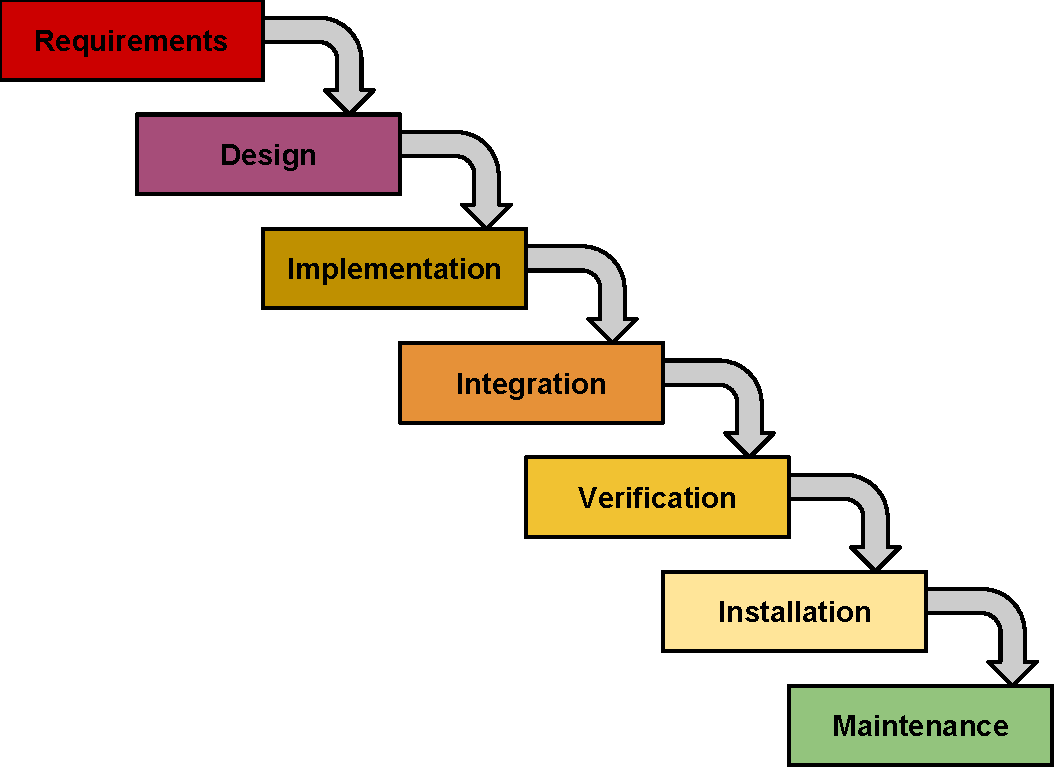
\includegraphics[scale=0.6]{../Figures/Waterfall-model.pdf}
\end{center}
\caption{Development cycle in Waterfall}
\label{figure:waterfall-model}
\end{figure}

The model is easily understandable, structured, and disciplined.
The clear distinction between project phases make it easier to monitor the progress of the project.
However, adopting Waterfall in real software projects can be challenging because it requires to be able to
foresee, in the early stages of the project, any problem that could arise later on and plan accordingly.
This is often a very hard task that requires great insight and expertise.

Waterfall may be suited to large-scale, expensive projects where 'going back' on design choices is not an
option and requirements are clearly established early on and then 'set in stone'.
However, many software projects nowadays fail to meet these conditions.

%-----------------------------------
%	SUBSECTION 2
%-----------------------------------
\subsection{Scrum Model}
%cite http://www.mountaingoatsoftware.com/agile/scrum

Scrum is an emerging agile development process which is mostly used in software development.
The Scrum approach, which could be described as both iterative and incremental, consists of multiple
sprints which last from two to four weeks. Sprints begin with a planning meeting and conclude with a review meeting.

During the sprint planning meeting team members produce a \emph{sprint backlog}: an artifact which defines a
set of concrete goals of the sprint and can be seen basically as a 'to-do' list tasks to be performed.
Such tasks, which in Scrum's terminology are called \emph{stories} are taken from the \emph{product backlog} which
is a prioritized list of the requirements of the product. Although a product backlog is usually made during the early
stages of the project, it is subject to change in order to accommodate new or modified requirements. 
The person in charge of populating and ordering the product backlog is the \emph{product owner}.

Each day in a sprint begins with a meeting called \emph{daily scrum}. 
During this meeting which is usually brief, everybody shares the work accomplished since the last daily
scrum and their plan for the day, mentioning eventual problems if any. 
A sprint concludes with a sprint \textit{review meeting} where the team evaluates the work done.

%If there are any problems the Scrum master is responsible to resolve the problem.
The whole process is supervised by the \textit{Scrum master} who has the responsability to
help other team members to perfom at their best and solve problems that might arise during the process.
Figure \ref{figure:scrum-workflow} shows the workflow in Scrum. \cite{Compendium}

\begin{figure}[h]
\begin{center}
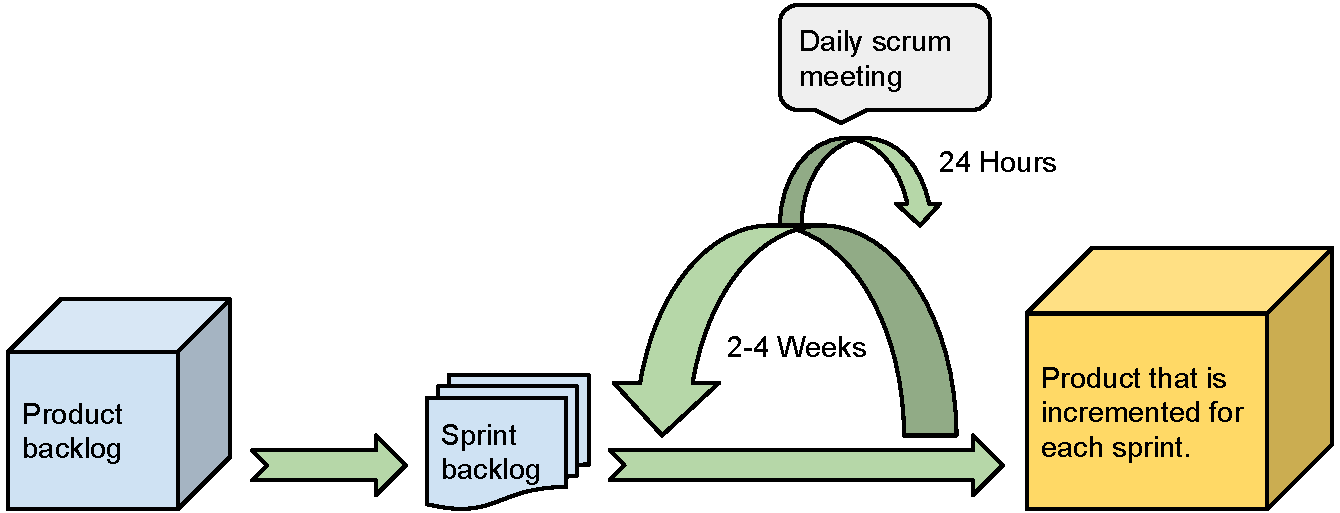
\includegraphics[scale=0.5]{../Figures/Scrum-workflow.pdf}
\end{center}
\caption{Scrum workflow}
\label{figure:scrum-workflow}
\end{figure}

%-----------------------------------
%	SUBSECTION 3
%-----------------------------------
\subsection{Conclusion}
\label{subsec:devprocess}

After discussing about possible alternatives, we decided to use Scrum based on the following considerations:

\begin{enumerate}
\item we didn't have a formal set of requirements from the beginning and we expected their nature to be volatile,
that is, subject to change throughout the duration of the project.

\item at the beginning of the project, our knowledge of both the problem and the technologies involved was
limited thus it would have been very risky to make decisions we wouldn't be able to adjust later.

\item given the size of the project and of our group, we wanted a development process with a small overhead.
Waterfall is notoriously not a process with a small overhead.

\item we had previous working experiences with Scrum, whereas our experience with Waterfall was only theoretical.

\item the customer suggested us to use an agile method.

\end{enumerate}

All in all, Scrum seemed to fit very well the nature of this project.
We thought that iterating the same activities over and over would have led to a natural improvement of our process and left a lot of possibilities to adjust the requirements and thus the design accordingly.
However, we made the following adjustment to the process in order to adapt it to our specific case:

\textbf{Daily scrum}\newline
We performed daily scrum on days we planned to work together: Mondays and Wednesdays.
Because everyone in the group had to attend courses, or to deliver assignments, or a job, or all these things, we couldn't work every day on the project. 
Since there was nothing to report, we didn't see the need for a daily scrum meeting.

\textbf{Sprint review meetings}\newline
Usually this meeting is held at the end of a sprint. 
In our case however, because our last meeting each week was on Wednesdays but we often worked on the project later during the rest of the week, we decided to combine the sprint review meeting with the sprint planning meeting (on Mondays every two weeks).


\section{Existing Solutions}
\label{section:existing-solutions}

This section describes existing solutions which have helped us get a better overview of technologies
and design patterns used to solve this kind of problem. 
What we present in this section are the ones we found most relevant and inspiring for our work.

%-----------------------------------
%	SUBSECTION 1
%-----------------------------------
\subsection{HealthVault}
%http://msdn.microsoft.com/en-us/healthvault/jj128027

HealthVault\cite{HealthVault} is Microsoft's online platform to collect, store and monitor personal health information. 
One of its most interesting features is interoperability with third-party solutions which are,
in HealthVault terminology and in this subsection hereafter, referred to as \textit{Apps}.

Examples of Apps include:
\begin{itemize}
\item smartphone and desktop applications
\item devices like step counters, blood glucose meters, weighting scales\ldots
\item third-party health services like Withings, \ldots
\end{itemize}

At the moment of writing, HealthVault supports more than 300 applications and 80 devices (in the U.S.).
Apps are used to populate a user's health record by collecting health measurements and parameters and, in turn,
make use of such information to provide services.
In order to connect to HealthVault, third-party applications need to be authorized by the user upon first use. 
Authorization can be restricted to a specific set of data: e.g. an App may be authorized to access weight and
glucose records but not allergies and pregnancies.

Thanks to a well documented XML-over-HTTP API and several software development kits (SDK)
for major mobile platforms and languages, it is easy for third-party developers to implement
interoperability with HealthVault in their application.

The API defines a set of data called \textit{things}.
Basically, a \textit{thing} represents a measurement of some health parameter e.g. heart rate, weight.
\textit{Things} are represented using XML, see an example below (a weight \textit{thing}).

\begin{lstlisting}[language=XML]
<weight>
  <value>
    <kg>60</kg>
    <display units="kg">132</display>
  </value>
  <when>
    <date>
      <y>1990</y>
      <m>1</m>
      <d>1</d>
    </date>
    <time>
      <h>1</h>
      <m>0</m>
      <s>0</s>
    </time>
  </when>
</weight>
\end{lstlisting}

Additionally, HealthVault supports exporting of data in industry-standard formats and storage of medical
imaging formats such as \textit{DICOM} and provides a degree of availability and redundancy.
Figure \ref{figure:hv-page} shows Ola Nordmann HealthVault's web page.

\begin{figure}[h]
\begin{center}
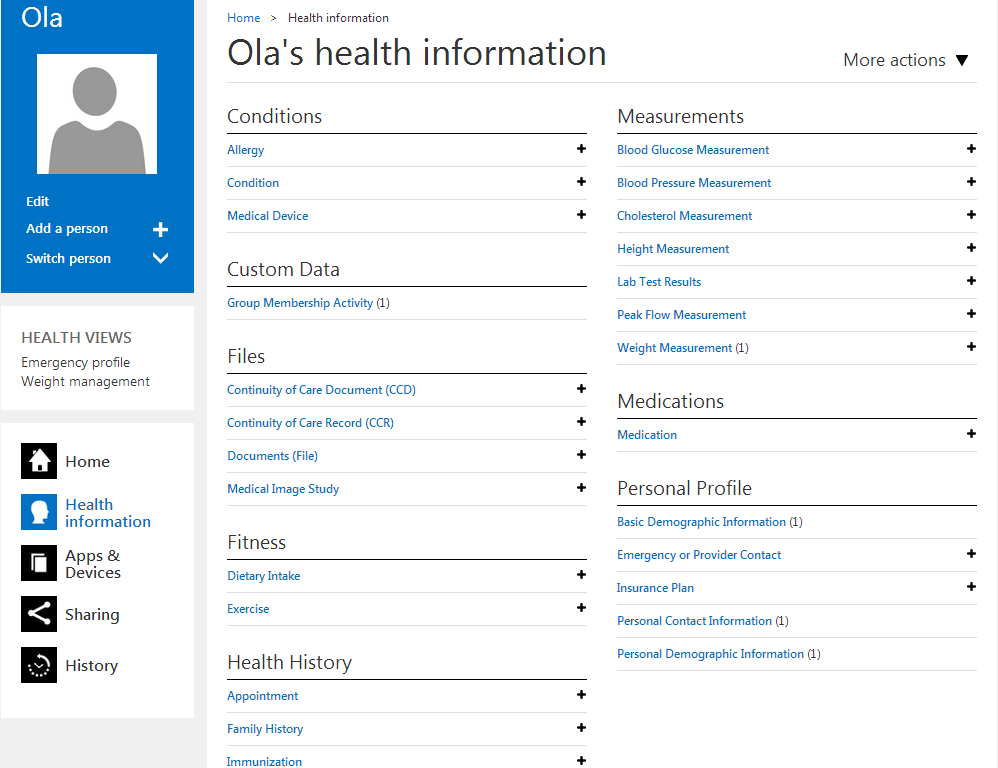
\includegraphics[scale=0.50]{../Figures/hv-page.png}
\end{center}
\caption{HealthVault web interface}
\label{figure:hv-page}
\end{figure}

%maybe we cant use this picture. it's good tho...
\iffalse
\begin{figure}[h]
\begin{center}
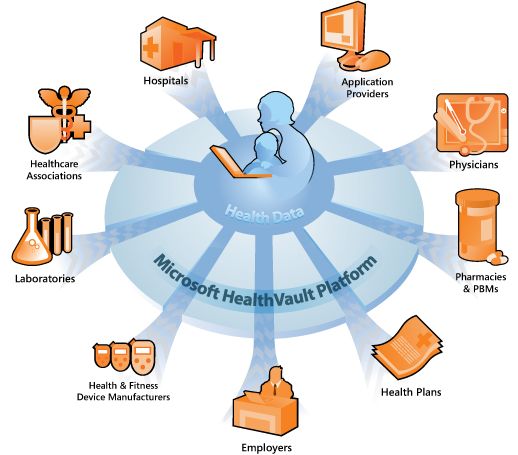
\includegraphics[scale=0.6]{../Figures/hv-cloud.png}
\end{center}
\caption{HealthVault apps}
\label{figure:hv-apps}
\end{figure}
\fi

%An HealthVault account can be linked to multiple individuals.

%-----------------------------------
%	SUBSECTION 2
%-----------------------------------
\subsection{human/api}
\label{section:humanapi}

The human/api is a RESTful web API for health data developed by human/api Inc.
Its aim is to offer a single access point to people's health information in order to facilitate developing
health applications. For this purpose, human/api collects people's health parameters (blood pressure, weight\ldots)
from a variety of third-party services (e.g. Withings) and devices (e.g. sensors) and normalizes it.
The data is then made available through a clean and well documented web API.
This has the benefit of providing a single service for application developers to authenticate against in order
to obtain users' health information, without having to integrate with multiple services individually.
Additionally, all data is represented using standardized models and format (JSON) of which we present an
example below. \cite{HumanAPI}

\begin{lstlisting}[language=JSON]
{
  "id": "string",
  "userId": "string",
  "time": "date",
  "value": {
    "diastolic": "int",
    "systolic": "int",
    "unit": "string"
  },
  "heartRate": "int"
}
\end{lstlisting}

%-----------------------------------
%	SUBSECTION 3
%-----------------------------------



%-----------------------------------
% SUBSECTION 4
%-----------------------------------
\subsection{Open eHealth Foundation}

The goal of Open eHealth Foundation is to create and share open source software components for the healthcare ICT industry.
One of their products is an integration platform called Open eHealth Integration Platform (IPF).
It is based on Apache Camel and has support for connecting systems in the eHealth domain. \cite{OpenEHealthFoundation}


%-----------------------------------
%	SUBSECTION 5
%-----------------------------------
\subsection{Conclusion}

The solutions presented in this subsection were of great influence in our work.
\verb|human/api| influenced our data models and representation as well as being a good example of how to implement security.
HealthVault, together with its SDKs proved to be a valuable example of a modern health integration platform.
We made use of HealthVault SDK to interact with the Microsoft's platform and were able to re-use a large portion of the code shipped as example.

%The android-heart-rate-monitor application was used to provide functionality that would have
%taken some effort to implement from scratch.


\section{Security concerns}

This section describes our studies about security.

\subsection{HIPAA - Health Insurance Portability and Accountability Act}

\begin{figure}[h]
\centering

\includegraphics[scale=0.50]{../Figures/hipaa2.png}
\caption{HIPAA logo}
\label{figure:HIPAA}
\end{figure}

HIPAA\cite{HIPAA} is an american act which, among other things, establishes some standards
for electronic health care. The \textit{privacy regulations} in HIPAA require
that a set of practices and precautions is put in place when trasferring, sharing
and handling health information electronically.
After discussing security with the customer we brought up the topic of HIPAA.
Even though there is no similar act in Norway, the customer believed that it could have been
valuable to discuss it and take it as starting point for our considerations about security. 

\textbf{Storage of data}\newline
HIPAA specifies that the hard drives used to store data must be encrypted and
kept safe from unauthorized physical access. HIPAA does not specify what type
of encryption should be used.

\textbf{Transfer of data}\newline
Data transfer should be carried out using a Secure Socket Layer\cite{SSL}
to prevent access by unauthorized people by means of encryption.

\textbf{Backup of data}\newline
Data should be backed-up in a exact and retrievable copies.
The frequency of backups should be appropriate for the data itself
taking into consideration how often is said data being updated and how it is being
used.

\textbf{Logging}\newline
Data access has to be logged in order to be able to monitor who
has accessed what and when.

\textbf{Security breaches}\newline
If a security breach happens, people whose data could have been compromised
should be notified. Depending on the severity of the breach, which could be
based on the amount of information disclosed or their sensibility,
a public announcement must be made.

\textbf{Authorization}\newline
HIPAA specifies that the user must be able to authorize access to his data,
which must be requested specifying not only the data itself, but also
an expiration for the requested authorization, its purpose and all parties
which request such authorization.

\subsection{Authentication}

There are multiple systems already in use in Norway for authenticating users. 
Some of the biggest systems are MinId, BankID, Buypass and Commfides.
The most widespread is BankID, with almost 3 million users at the moment
writing\footnote{See https://www.bankid.no}.
It would be worth considering to use BankID to authenticate citizens because
it is already adopted by most of them.


\subsection{OAuth 2.0}

OAuth 2.0\cite{OAuth} is a standard for authorization. %third-party applications to access data on a system.
%securing that could potentially be used for our integration platform.
%OAuth 1.0 is outdated, and hence we will mainly focus on OAuth 2.0 in this section.
%OAuth is used to authorize third party applications access to a system.
%In our case this could for example be only access to the API concerning heart rates or weights in NIPEN.

%\subsection{What is OAuth?}

The scenario where an application wants to interact with an API provider to obtain information
about a user is becoming more and more common: think of Facebook and all the applications that use data
which Facebook provides. It would certainly be a bad idea for a user to share his account credentials
with many third-party applications because doing so would enable them to do what they want with it.

\iffalse
% the user doesn't always want to give his/hers credentials to these applications.
Lets say that a user wants user an application that is able to upload images to his/hers
Facebook account but doesn't feel confident about giving the applications his Facebook credentials.
%The user doesn't want to give the application the credentials for facebook.
This would be highly insecure, since once the application has the authentication information
of a user it is able to do whatever it wants with the account.
\fi

OAuth tries to solve this kind of problem authorizing third-party applications to access
user's information, or part of it, on a server without providing any account credentials.

For this purpose third-party application developers need to register their application
with the API provider. This might include name of the application, a description, logo\ldots
This is to allow applications to be authenticated and controlled by the API provider itself.
Upon registration, a client-ID to be used for authentication is assigned to the application.

Then, in order to be authorized to access some user's data, the application redirects the
user to the API provider's page where he can authenticate himself without actually providing
any credentials to the application. Then he proceeds to authorize the application to access (or not)
a specific set of data. The application is finally returned a token representing the level
of authorization granted. Authorization can be revoked by the user at any time.


%For this purpose it makes use of a token based system, where the application receives a token specifying
%the authorization level granted to it by the user.

%A redirect URI also needs to be registered.
%This URI needs to use TLS, i.e. must begin with \textit{https}.
%This address is used to send an authentication token from the system to the application.
%After the registration, the application should receive a client ID which is used to identify the application at the system.
\iffalse
Now users should be able to connect the application with theirs account on the system.
The way it works is that through the application they will be sent to a website of the system the application wants to connect with.
There the user will be asked if he/she wants to grant permissions to the application.
If the user agrees, then he/she will be redirected to the applications specified redirect URI with an access token as a parameter.
The application will now use this token to access the system.
When the user doesn't want the application to have access to the system any more, he/she can simply disallow the applications access through the systems website.
\fi

An example of how OAuth works is given in figure \ref{figure:oauth-in-a-nutshell}.
In this example we see a website that wants to send images to a user's Facebook account.
If the user authorizes the application through Facebook, then Facebook will send an access
token to the website. Then \textit{www.ImageToFacebook.com} will be able to send images to the
users account, providing their access token for authorization.
%The user should be able to disallow the website access at any time on Facebooks website. 

\begin{figure}[h]
\centering
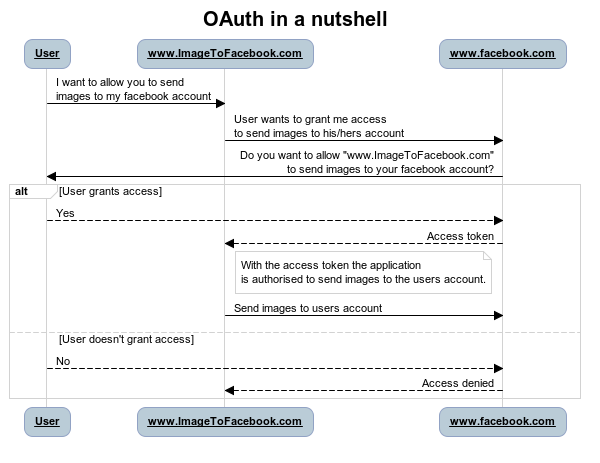
\includegraphics[scale=1.0]{../Figures/oauth-in-a-nutshell.png}
\caption{OAuth in a nutshell}
\label{figure:oauth-in-a-nutshell}
\end{figure}


\clearpage
%----------------------------------------------------------------------------------------
%	SECTION 4
%----------------------------------------------------------------------------------------
\section{Involved technologies}
\label{section:used-technologies}

In this section we present some relevant technologies we took into consideration for our product.

%-----------------------------------
%	SUBSECTION 1
%-----------------------------------
\subsection{Programming languages}

\textbf{Java}\cite{Java}\newline
Java is a general-purpose programming language that it can be used in a wide variety of application domains.
It is platform independent, and thus makes it easy to develop software once and deploy it on different operative systems.
Web programming is one of the domains that Java is used in, making it possible to write a service
that runs in the back-end of a website (using JSP).
%The web services created with Java allows creating a bridge between the database and the front-end. 
%This makes it possible to create a communication between the user and the database at the server.


%-----------------------------------
%	SUBSECTION 2
%-----------------------------------
\subsection{Database}
In this section we present those technologies related to database development.

\textbf{MySQL}\cite{MySQL}\newline
MySQL is one of the most widely used relational database management system.
The Community Edition of MySQL is open source and freely available.
It is developed to handle large databases and support many users at the same time.%. and it is also scalable.
It makes it possible to store and retrieve data in an efficient and structured manner. 

\textbf{Microsoft SQL server}\newline
Microsoft proprietary SQL server implementation. Needless to say, it only runs of Microsoft
Windows. A freeware \textit{Express} version is available.

\textbf{Apache Derby}\newline
Apache Derby is a relational database management system developed by the Apache foundation
and released under the Apache License 2.0.

\textbf{MySQL Workbench}\newline
MySQL Workbench is a free-to-use tool which allows to easily manage MySQL databases.
We used MySQL Workbench for database design and deployment both locally (for testing) and remotely (production).


%-----------------------------------
%	SUBSECTION 3
%-----------------------------------
\subsection{Web development}
In this section we present those technologies related to web development.

\textbf{Spring Framework}\cite{SpringFramework1}\cite{SpringFramework2}\newline
The Spring Framework is an a Java-based application framework and inversion of control container.
Spring is widely used and freely available under Apache License 2.0\footnote{See http://www.apache.org/licenses/LICENSE-2.0}.
%We use the Spring framework to set up a RESTful service and to handle the data access from the database. 

\textbf{Apache Tomcat}\cite{ApacheTomcat}\newline
Apache Tomcat is a mature, reliable and freely avaialable HTTP web server implementation licensed
under the Apache License 2.0. Additionally, Apache Tomcat runs on a variety of different platforms.
Numerous companies and organizations use Apache Tomcat for large-scale and mission-critical web applications.

\textbf{Microsoft IIS}\cite{}\newline
Microsoft Internet Information Services (IIS) is Microsoft's proprietary web server solution.
It is stable, mature and well documented. It is shipped as an integral part of Windows operative system (sharing thus
its same license), although a freeware, stand-alone version is also available. Needless to say, Microsoft IIS only
runs on Windows.

\textbf{Microsoft WCF}\cite{}\newline
Microsoft's WCF is Microsoft's framework for developing applications that communicate over a network.
WFC uses Microsoft's proprietary .NET framework to develop web applications.

\textbf{HTML5}\cite{HTML5}\newline
HTML is the standard World Wide Web's markup language, HTML5 being the latest HTML version at the moment of writing.
It is used to structure and visualize web pages on the internet. By writing a document with HTML a
web browser is later on able to interpret the document and visualize it in a structured manner. 

\textbf{CSS3}\cite{CSS3}\newline
CSS describes the look and format of a document written in HTML.
It allows one to use different fonts, colors and adjust the layout of a web page.
By using CSS and separating it from the HTML, it is possible to allow multiple pages share the same style
making them easier to maintain and adapt to different environments. 

\textbf{Bootstrap}\cite{Bootstrap}\newline
Bootstrap contains HTML and CSS templates for web designers.
This makes it easier to make a good looking web page without putting too much effort into the design.

\textbf{JavaScript}\cite{JavaScript}\newline
JavaScript is an interpreted computer programming language that runs in the browser of the user.
It is allowed to make changes in the HTML DOM, interact with the user, control the browser and communicate asynchronously.
Since it can communicate with the server asynchronously, it makes the web page more dynamic.
What this means is that a web page can acquire new information and change the site without reloading.

\textbf{jQuery}\cite{jQuery}\newline
jQuery is a JavaScript library for manipulating and traversing the HTML DOM.
All the features available in jQuery are achieved using pure JavaScript, but jQuery helps
the developer to implement the different features in an easier way:
e.g. it contains predefined methods for event handling and animation.
It also makes it easier to communicate with the server through AJAX. 

\textbf{Chart.js}\cite{Chartjs}\newline
Chart.js is a JavaScript library for creating graphs and charts.
It helps the developer to easily visualize data through different types of graphs.
The library has support for different types of two dimensional data, e.g. value per time.
It also has the ability to display multiple graphs in the same chart. 


\subsection{Mobile Technologies}
In this section we present those technologies related to mobile development.

\textbf{Android SDK}\cite{AndroidSDK}\newline
The Android SDK contains the tools necessary for developing, debugging and testing a Android applications.
%With the SDK it is possible to write and modify applications for an Android phone.

\textbf{android-heart-rate-monitor}\cite{AndroidHeartRateMonitor}\newline
\label{subsec:hr}
android-heart-rate-monitor is an open source (Apache 2.0 license) Android application that can be used to measure
the user heart rate. The application uses the phone's camera and flash to compute 'redness' levels on user's fingertips. 
These are supposed to increase in correspondence with heartbeats. The application computes an average 'redness' value
and uses that to detected heartbeats and calculate a beats per minute (BPM) measurement.


%% redudant with tools section. they are tools not really 'technologies'

\iffalse
\subsection{Other Technologies}

\textbf{Maven}

Maven is a software tool for managing a programming project.
It has the ability to build and compile programming code based on the content of a POM (Project Object Model) file.
It keeps track of all the frameworks used, and is able to download them before building the project. \cite{Maven}

\textbf{Git}

Git is a version control system that is free and open source.
This is an important tool to keep track of all the changes made to the source code, it also makes it easier for multiple developers to work on the same source.
Git makes it easy to roll back changes made to the code, in case something was wrongly implemented.
It also has the possibility to divide the project into different branches.
Which means that the code can be copied into multiple different places, and developed separately in cases where trying out different solutions is necessary.
If a good solution is made, the branch can later on be merged together with the main branch.
It is also possible to have a branch for release versions and a development branch. \cite{Git}
\fi

\subsection{Conclusion}

There were, of course, a number of alternatives to most of these technologies and the whole
report wouldn't be enough to describe them all. The reasons behind our choices have been very practical.
We didn't want, if possible, to limit our product to one single platform so we chose to avoid Microsoft's solutions.
Additionally, we were limited to those solutions which were freely available to us.
We tried, when possible, to opt for technologies which were well documented and that we were not
totally unfamiliar with in order minimize the time we would spend to figure out how to make them work.
We don't claim that our choices of employed technologies are the 'best' choices possible,
but we found them appropriate for our case.

\iffalse
We chose the technologies specified above based on our earlier experience and what we found most appropriate for our solution.
Before we started this project we discussed our competencies.
This was of great help in choosing the right technologies that were going to be used.
Most of us already had some different degree of experience in most of the technologies mentioned above.
This made it much easier for us to chose the right set of frameworks and languages to work with.
\fi

%----------------------------------------------------------------------------------------
%	SECTION 5
%----------------------------------------------------------------------------------------
\section{Service oriented architectures}

The architecture of the service itself will play an important factor in its scalability and complexity.
In this section we will cover some methods that can be used for interaction between clients and servers. 

\subsection{REST}\cite{REST}
\label{subsec:rest}

REST, is an acronym from Representational State Transfer and is basically an architectural style where clients
(user agents) make requests of services (endpoints) to servers.

REST is based on a set of principles:
\begin{itemize}
\item Clients interact with resources. The term 'resource' refers to anything that can have a name and a representation.
      A resource is addressed via a unique Uniform Resource Identifier (URI).
\item All informations regarding a resource are contained in the resource itself: resources are self-descriptive.
      Because all information needed to process a request on any resource is contained in the resource itself,
      the services can be stateless.
\item Resources can be accessed by client using HTTP methods such as \verb|GET|, \verb|POST|, \verb|PUT| and \verb|DELETE|.
      Each of these methods corresponds to an operation:
			\begin{itemize}
				\item \verb|GET|: returns all the elements of a collection, or a specific element if its ID is specified.
				\item \verb|POST|: creates a new entry in a collection or a new element.
				\item \verb|PUT|: is to replace a collection or a particular element in it.
				\item \verb|DELETE|: deletes an entire collection or a particular element in it.
			\end{itemize}
\item Resources can contain link to other resources.
\end{itemize}

This type of service does not have any specific requirements on how the data should be formatted or what it should look like.
What described, results in a number of advantages.

\textbf{Scalability}\newline
Because RESTful services are stateless, they are generally lightweight in resources and easy to scale up.

\textbf{Caching}\newline
Requests sent to RESTful services are made using HTTP methods and HTTP \verb|GET| results are cached, this can
lead to further scalability capabilities and speed.

\textbf{Interoperability}\newline
REST only requires an HTTP connection.

\textbf{Idempotency and nilpotency}\newline
%\verb|PUT| and \verb|DELETE| methods are idempotent. This means that one nullifies the effects of the other.
\verb|PUT| and \verb|DELETE| methods are idempotent. 
This means that after executing these methods once, later execution of this methods will have no effect.
Because an element can only be replaced or deleted once.
\verb|GET| is nilpotent, meaning that it has no side effects. These are desirable features considering
that over a network information is likely to get lost or sent multiple times and it would not unlikely for an operation
to be executed twice. %Having the possibility to revert changes made to the data could be valuable,
%as well as having a nilpotent operator that has no effect on data itself.

\textbf{Simplicity}\newline
REST is simple and that is one big advantage.

\subsection{SOAP}\cite{SOAP}
\label{subsec:soap}
SOAP (Simple Object Access Protocol) is a protocol for exchanging information between web services in a network.
SOAP makes heavy use of XML for communication. There are strict rules on how the XML data should be formatted.
A SOAP message constists of different parts: a header, a body, a fault and an envelope. Some of these
are mandatory while some are optional. Table \ref{table:soap-message} shows an overview of these parts.

\begin{table}[h]
\begin{center}
\begin{tabular}{ | l | l | c | }
  \hline
  Part  & Description & Required \\
  \hline\noalign{\smallskip}\hline
  Header & Contains header informations & No \\
  Body   & Represents the body of the message   & Yes \\
  Fault  & Describes eventual errors occurred during processing  & No \\
  Envelope & Wraps the whole message & Yes \\
  \hline
\end{tabular}
\end{center}
\caption{SOAP message parts}
\label{table:soap-message}
\end{table}

The structure of a SOAP message is illustrated in figure \ref{figure:soap-message}.

\begin{figure}[h]
\begin{center}
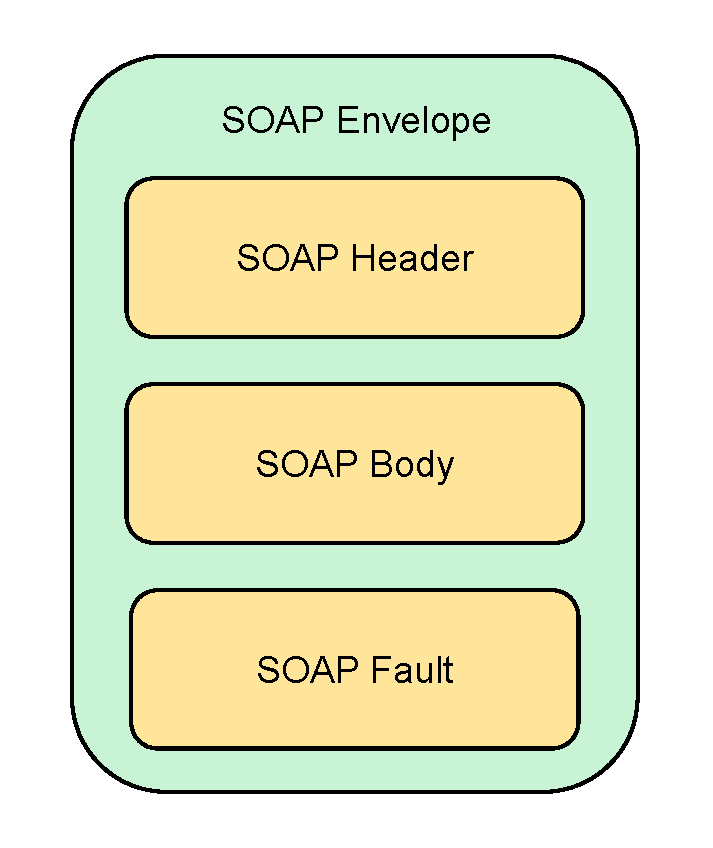
\includegraphics[scale=0.50]{../Figures/SOAP.pdf}
\end{center}
\caption{SOAP message structre}
\label{figure:soap-message}
\end{figure}


%It needs to contain an envelope and a body, in addition it can also contain a header and a fault.
%The envelope tells that the message that is being sent is a SOAP message, and the body contains the main information
%that is being sent. A header can contain header information, and fault tells if there were some errors during the
%processing of the message. Figure \ref{} shows a SOAP message.

SOAP has three major characteristics:
\begin{enumerate}[1.]
\item it is neautral, in the sense that it doesn't specify a mean to transport data
\item it is indipendent, meaning that it allows for any programming model
\item it is extensible
\end{enumerate}

Furthermore, it has a number of advantages over over other formats like pure XML and JSON:
\begin{itemize}
\item SOAP messages can have multiple recipients
\item parts of a SOAP message can be encrypted to be readable by certains recipients only
\item SOAP allows to represent more generic data structures
\item SOAP messages are guaranteed to be delivered
\end{itemize}

\subsection{Conclusion}
\label{subsec:soa-conclusion}
All in all, we found REST more suitable for our product for a number of reasons.
In the first place, REST is simpler than SOAP and we didn't need all the complexity introduced by the latter.
Additionally, REST is generally considered more lightweight due to its use of a less verbose data
represention (JSON vs XML). Both these factors contribute to a better scalability.
We were sure that REST would be available on any platform since what is needed
is really only an HTTP library. Furthermore, we all had some kind of experience with
REST APIs but none of us never had any experience with SOAP.

%Since SOAP uses XML and has strict rules for how the data format should be, we find a
%RESTful service more appealing for our solution.
%With rest it is possible to send raw JSON strings with a custom defined format.
%JSON strings are much easier to handle and manipulate on a web based front-page, by using JavaScript.

%----------------------------------------------------------------------------------------
%	SECTION 6
%----------------------------------------------------------------------------------------
\section{Testing}
\label{section:testing}

%In this section we are going to go through some of the testing frameworks used in our project.
In this section we are going to go through some of the testing frameworks explored during our preliminary study.

\subsection{JUnit}

JUnit is a Java framework for writing tests. It is also a good tool when using test driven development.
With help of this framework it is possible to write tests for different parts of the code, then check if it runs as it should.
It is also possible to use JUnit with Maven.
When doing so it will first run all the tests, and if the tests are successful the application will be executed. \cite{JUnit}

\subsection{Jasmine}

Jasmine is a framework for testing JavaScript code.	
It doesn't require a DOM and is also not dependent on any other frameworks. \cite{Jasmine}

\subsection{Conclusion}

When using test driven development it is important to have some frameworks for testing the code.
New bugs are often introduced to applications when extending it with new functions and features.
With help of the technologies mentioned above it is much easier to find the new bugs, and hence fix them quicker. 

\chapter{Requirements specification}

\label{ch:requirements}
\lhead{Chapter 4. \emph{Requirements specification}}

This chapter provides a description of project's stakeholders and requirements, both
functional and non-functional. Requirements will be presented textually and with the aid of
some use-case diagrams. 

Throughout this chapter both requirement's priority and complexity have a textual description which can be
\begin{itemize}
\item High
\item Medium (abbrev. Med)
\item Low
\end{itemize}

The use of such terms is described in table \ref{table:priorities} for priorities
and table \ref{table:complexity} for complexities.
\begin{table}[h]
\begin{center}
\begin{tabular}{ | r | p{11.5cm} | }
  \hline
  \textbf{Priority} & \textbf{Description} \\
  \hline\noalign{\smallskip}\noalign{\smallskip}\hline
  \textbf{High} & An essential requirement.\newline
  The product \textbf{must fulfill} the requirement in order to be satisfactory. \\
  \textbf{Medium} & A useful requirement.\newline
  The product \textbf{should fulfill} the requirement to maximise effectiveness. \\
  \textbf{Low} & A desiderable requirement.\newline
  The product \textbf{could fulfill} the requirement to be more interesting to some stakeholders. \\
  \hline
\end{tabular}
\end{center}
\caption{Priority descriptions}
\label{table:priorities}
\end{table}

\begin{table}[h]
\begin{center}
\begin{tabular}{ | r | p{11.5cm} | }
  \hline
  \textbf{Complexity} & \textbf{Description} \\
  \hline\noalign{\smallskip}\noalign{\smallskip}\hline
  \textbf{High} & The requirement is difficult to implement.\newline
  It will take a considerable amount of time. (more than 45 hours) \\
  \textbf{Medium} & The requirement is moderately difficult.\newline
  It will take some time. (from 15 to 45 hours) \\
  \textbf{Low} & The requirement is easy and can be achieved\newline
  in a short amount of time. (15 hours or less) \\
  \hline
\end{tabular}
\end{center}
\caption{Complexity descriptions}
\label{table:complexity}
\end{table}


%-----

\section{Stakeholders}
\label{section:stakeholders}
A project's stakeholders are those people that have an interest in the project.
%This section contains a description of project's stakeholders: those people that have an interest in it.
We have identified five stakeholders for this project and presented them below.
%A short description\iffalse of the role\fi of each stakeholder is given, and what concerns they might have.

\subsection{Customer}
The customer is\iffalse the one that is\fi going to steer the project toward the direction he pleases.
The interest of the customer is to receive a product that will be as useful as possible for him.
% us to the solution he wants.
%His concern is that we should maintain an effective and good communication with him, so he understands our progress.
His concern is to be able to communicate well with the group and make his expectations for the product
and for the documentation clear.
%We should also document the advancement we are making and have a clear system architecture for him.
%His main concern is to get a working prototype of our system according to his requirements.

\subsection{Course's staff}
The course's staff will evaluate our project. Their interest is that we, as a group of students,
gain valuable knowledge and experience in a number of areas related to software development.
It is their interest to make the criterias behind grading clear to the students
so that their effort is focused on the objectives of the course.
They expect all the deliverables to be submitted on schedule.
%Good communication is also of importance, and of course that we will learn something from the course.

\subsection{Our group}
As a group made up of good students, our main interest is to gain the most out of our tuition.
We have therefore committed to pass this course with a good profit and will give our best
to satisfy the customer and produce a good documentation.
%We are going to write the report and implement our applications.
%Our concern is to fulfil the requirements of our customer, finish the report and have a good presentation
%that reflects our work.

\subsection{Third party developers}
The third party developers are going to integrate their applications with our system, or eventually
extend some of its functionality. Their concern is that our integration platform is well documented
in order to be easy to integrate with or to extend.

\subsection{Users}
The users are going to use the following products: the front-end and Android applications.
%They are the users of our front-end and both Android applications.%heart rate application and our weight application.
It is their concern that their data is easily available and is visualized in an intuitive and comprehensible way.
They should be able to push heart rate and weight measurements to the integration platform smoothly and without
any explicit training.

%-----

\section{Requirements}

The product consisted of different, interoperable systems including:
\begin{enumerate}[1.]
\item an integration platform, here and thereafter referred to as \textit{NIPEN}
\item a graphical front-end for NIPEN in the form of a web page
\item an Android application referred to as simply \textit{Heart rate}
\item an Android application referred to as simply \textit{Weight}
\item a web service referred to as \textit{HealthVault integration service}
\end{enumerate}

Each requirement also had a priority which helped us identify the focus of our work.
Priorities could be reviewed based on customer's feedback. We tried to prioritize those requirements corresponding
to the functionality that the customer expressed most interest about. In order to better organize
our workload we also estimated a complexity for each requirement.

\newpage
\subsection{Functional requirements}
\label{section:functionalreq}

This section contains a description the functional requirements for the product.

\textbf{Functional requirements for NIPEN}

\begin{table}[h]
\begin{center}
\begin{tabular}{ | r | p{11.5cm} | }
  \hline

  \textbf{ID} & FIP1 \\
  \hline\noalign{\smallskip}\hline
  \textbf{Description}  & NIPEN shall support API endpoints for receiving heart rate data
                          models expressed as JSON strings.\\
  \textbf{Complexity}   & Med \\
  \textbf{Priority}     & High \\
  \hline\noalign{\smallskip}\noalign{\smallskip}\hline

  \textbf{ID} & FIP2 \\
  \hline\noalign{\smallskip}\hline
  \textbf{Description}  & NIPEN shall support API endpoints for receiving
                          weight data models expressed as JSON strings.\\
  \textbf{Complexity}   & Med \\
  \textbf{Priority}     & High \\
  \hline\noalign{\smallskip}\noalign{\smallskip}\hline

  \textbf{ID} & FIP3 \\
  \hline\noalign{\smallskip}\hline
  \textbf{Description}  & NIPEN shall support API endpoints for forwarding
                          stored heart rate measurements as JSON models.\\
  \textbf{Complexity}   & Med \\
  \textbf{Priority}     & High \\
  \hline\noalign{\smallskip}\noalign{\smallskip}\hline

  \textbf{ID} & FIP4 \\
  \hline\noalign{\smallskip}\hline
  \textbf{Description}  & NIPEN shall support API endpoints for forwarding
                          stored weight measurements as JSON models.\\
  \textbf{Complexity}   & Med \\
  \textbf{Priority}     & High \\

  \hline
\end{tabular}
\end{center}
\caption{Functional requirements for NIPEN}
\label{table:reqip}
\end{table}

\textbf{Functional requirements for the web frontend}

\begin{table}[h]
\begin{center}
\begin{tabular}{ | r | p{11.5cm} | }
  \hline

  \textbf{ID} & FW1 \\
  \hline\noalign{\smallskip}\hline
  \textbf{Description}  & The web frontend shall display the data stored by NIPEN using charts.\\
  \textbf{Complexity}   & Med \\
  \textbf{Priority}     & High \\
  \hline\noalign{\smallskip}\noalign{\smallskip}\hline

  \textbf{ID} & FW2 \\
  \hline\noalign{\smallskip}\hline
  \textbf{Description}  & The web frontend shall use Helsenorge color palette. \\
  \textbf{Complexity}   & Low \\
  \textbf{Priority}     & Low \\
  
  \hline
\end{tabular}
\end{center}
\caption{Functional requirements for the web frontend}
\label{table:reqfrontend}
\end{table}

\newpage

\textbf{Functional requirements for Heart rate application}

\begin{table}[h]
\begin{center}
\begin{tabular}{ | r | p{11.5cm} | }
  \hline

  \textbf{ID} & FHR1 \\
  \hline\noalign{\smallskip}\hline
  \textbf{Description}  & The application shall measure user's heart rate using the device camera.\\
  \textbf{Complexity}   & High \\
  \textbf{Priority}     & High \\
  \hline\noalign{\smallskip}\noalign{\smallskip}\hline

  \textbf{ID} & FHR2 \\
  \hline\noalign{\smallskip}\hline
  \textbf{Description}  & The application shall display the measurement on screen. \\
  \textbf{Complexity}   & Low \\
  \textbf{Priority}     & High \\
  \hline\noalign{\smallskip}\noalign{\smallskip}\hline

  \textbf{ID} & FHR3 \\
  \hline\noalign{\smallskip}\hline
  \textbf{Description}  & The application shall forward the data to NIPEN using its REST endpoint.\\
  \textbf{Complexity}   & Med \\
  \textbf{Priority}     & High \\
  
  \hline
\end{tabular}
\end{center}
\caption{Functional requirements for heart rate application}
\label{table:reqheartrate}
\end{table}


\textbf{Functional requirements for Weight application}

\begin{table}[h]
\begin{center}
\begin{tabular}{ | r | p{11.5cm} | }
  \hline
  
  \textbf{ID} & FHV1 \\
  \hline\noalign{\smallskip}\hline
  \textbf{Description}  & The application shall fetch weight measurements from HealthVault. \\
  \textbf{Complexity}   & Med \\
  \textbf{Priority}     & High \\
  \hline\noalign{\smallskip}\noalign{\smallskip}\hline

  \textbf{ID} & FHV2 \\
  \hline\noalign{\smallskip}\hline
  \textbf{Description}  & The application shall display the weight measurements it has fetched. \\
  \textbf{Complexity}   & Low \\
  \textbf{Priority}     & Med \\
  \hline\noalign{\smallskip}\noalign{\smallskip}\hline

  \textbf{ID} & FHV3 \\
  \hline\noalign{\smallskip}\hline
  %\textbf{Description}  & The application shall forward the data to the IP using the web API. \\
  \textbf{Description}  & The application shall forward weight measurements to NIPEN using the web API. \\
  \textbf{Complexity}   & Low \\
  \textbf{Priority}     & High \\

  \iffalse
  ID & Description & Difficulty & Priority\\
  \hline\noalign{\smallskip}\noalign{\smallskip}\hline
  FHV1	& The application shall fetch weight data from HealthVault.						      & Med	& High \\
  FHV2	& The application shall show the user the data it has fetched.              & Low	& Med \\
  FHV3	& The application shall forward the data to NIPEN using its REST endpoint. & Med	& High \\
  \fi

  \hline
\end{tabular}
\end{center}
\caption{Functional requirements for the weight application}
\label{table:reqweight}
\end{table}

\newpage
\textbf{Functional requirements for HealthVault Integration Service}

\begin{table}[h]
\begin{center}
\begin{tabular}{ | r | p{11.5cm} | }
  \hline
  
  \textbf{ID} & FHIS1 \\
  \hline\noalign{\smallskip}\hline
  \textbf{Description}  &  The user shall be able to turn the application on and off. \\
  \textbf{Complexity}   & Low \\
  \textbf{Priority}     & High \\
  \hline\noalign{\smallskip}\noalign{\smallskip}\hline

  \textbf{ID} & FHIS2 \\
  \hline\noalign{\smallskip}\hline
  \textbf{Description}  & When on, the applicatin shall fetch weight data from HealthVault and
                          forward it to NIPEN using its web API. \\
  \textbf{Complexity}   & High \\
  \textbf{Priority}     & High \\
  \hline\noalign{\smallskip}\noalign{\smallskip}\hline

  \textbf{ID} & FHIS3 \\
  \hline\noalign{\smallskip}\hline
  \textbf{Description}  & The application shall allow the user to manually send weight measurements to HealthVault. \\
  \textbf{Complexity}   & Low \\
  \textbf{Priority}     & Med \\

\iffalse
\begin{table}[H]
\begin{center}
\begin{tabular}{ | c | p{9cm} | c | c |}
  \hline
  ID & Description & Difficulty & Priority\\
  \hline\noalign{\smallskip}\noalign{\smallskip}\hline
  FHIS1	& The application shall send weight data to HealthVault.						   & Low	& Low \\
  FHIS2	& The application shall fetch weight data from HealthVault regularly.		       & Med	& High \\
  FHIS3	& The application shall forward new weight data to NIPEN using its REST endpoint. & Med	& High \\
  \hline
\end{tabular}
\end{center}
\caption{Functional requirements for HealthVault Integration Service}
\label{table:reqwebservice}
\end{table}
\fi

  \hline
\end{tabular}
\end{center}
\caption{Functional requirements for HealthVault Integration Service}
\label{table:reqwebservice}
\end{table}

%-----
\newpage
\subsection{Non-functional requirements}
\label{section:nonfunctionalreq}

This section outlines non-functional requirements (quality attributes) for the product.
In order to provide a better overview, we have organized them in categories.

\begin{table}[h]
\begin{center}
\begin{tabular}{ | r | p{11.5cm} | }
  \hline
  
  \textbf{ID} & NF1 \\
  \hline\noalign{\smallskip}\hline
  \textbf{Category}			&	Documentation\\
  \textbf{Description}	& The system shall be thoroughly documented by the project report \\
  \textbf{Complexity}		& High \\
  \textbf{Priority}			& High \\
  \hline\noalign{\smallskip}\noalign{\smallskip}\hline

  \textbf{ID} & NF2 \\
  \hline\noalign{\smallskip}\hline
  \textbf{Category}			&	Documentation\\
  \textbf{Description}	& Although security and privacy are not requirements for the product they
													are important topics to be discussed in the documentation. \\
  \textbf{Complexity}		& Med \\
  \textbf{Priority}			& High \\
  \hline\noalign{\smallskip}\noalign{\smallskip}\hline

  \textbf{ID} & NF3 \\
  \hline\noalign{\smallskip}\hline
  \textbf{Category}			&	Open-source\\
  \textbf{Description}	& The product shall be released under a permissive license approved by the product owner. \\
  \textbf{Complexity}		& Med \\
  \textbf{Priority}			& Med \\
  \hline\noalign{\smallskip}\noalign{\smallskip}\hline
  
  \textbf{ID} & NF4 \\
  \hline\noalign{\smallskip}\hline
  \textbf{Category}			&	Interoperability \\
  \textbf{Description}	& The system shall provide a good degree of interoperability.
  												Third party application developers should be put in the condition to develop
  												third party (interoperable) solutions rapidly. \\
  \textbf{Complexity}		& High \\
  \textbf{Priority}			& High \\

  \textbf{ID} & NF5 \\
  \hline\noalign{\smallskip}\hline
  \textbf{Category}     & Interoperability \\
  \textbf{Description}  & A number of two or three prototype applications shall be developed in order to showcase
                          the functionality of the system \\
  \textbf{Complexity}   & High \\
  \textbf{Priority}     & High \\
  \hline\noalign{\smallskip}\noalign{\smallskip}\hline
  
  \textbf{ID} & NF6 \\
  \hline\noalign{\smallskip}\hline
  \textbf{Category}     & Accessibility \\
  \textbf{Description}  & The web-frontend should have a good degree of accessibility.
                          It should have a rather simple design and use a customer-provided palette. \\
  \textbf{Complexity}   & Low \\
  \textbf{Priority}     & Low \\

  \hline
\end{tabular}
\end{center}
\caption{Non-functional requirements}
\label{table:nonfunc}
\end{table}

\iffalse
\begin{table}[h]
\begin{center}
\begin{tabular}{ | r | p{11.5cm} | }
	\hline

  \textbf{ID} & NF5 \\
  \hline\noalign{\smallskip}\hline
  \textbf{Category}     & Interoperability \\
  \textbf{Description}  & A number of two or three prototype applications shall be developed in order to showcase
                          the functionality of the system \\
  \textbf{Complexity}   & High \\
  \textbf{Priority}     & High \\
  \hline\noalign{\smallskip}\noalign{\smallskip}\hline
	
	\textbf{ID} & NF6 \\
  \hline\noalign{\smallskip}\hline
  \textbf{Category}			&	Accessibility \\
  \textbf{Description}	& The web-frontend should have a good degree of accessibility.
  												It should have a rather simple design and use a customer-provided palette. \\
  \textbf{Complexity}		& Low \\
  \textbf{Priority}			& Low \\
	
	\hline
\end{tabular}
\end{center}
\caption{Non-functional requirements (cont.)}
\end{table}
\fi

% -----

\section{Requirements Validation}
\label{section:reqvalidation}

This section contains some considerations we made when defining requirements to ensure their validity\cite{Sommerville9}.

\textbf{Comprehensibility}\newline
It is important that requirements are expressed in a way that is understandable by the customer.
We have thus submitted a list of both functional and non-functional requirements of the system
to the customer for approval. Because requirements were subject to change due to the nature of the project
itself, the customer has reviewed them multiple times.

\textbf{Verifiability}\newline
It is crucial that a requirement can be tested. If a requirement can't be tested, it is not a valid requirement.
We have kept this in mind while formalising requirements.

\textbf{Adaptability (changeability)}\newline
We expected requirements to change multiple times during development.
For this reason we started with a set of high-level requirements to be later refined and improved.
This would allow the requirements to change without having a big impact on the progress of the project.

%-----

\newpage
\section{Use cases}
\label{section:usecases}

This section provides  the different use cases of our applications.
The section consists of use cases for NIPEN, front-end, heart rate application, weight application and the HealthVault integration service.

\subsection{NIPEN}

A use case diagram for NIPEN is given in figure \ref{figure:use-case-diagram-nipen}.
The integration platform (i.e. NIPEN) should be able to receive weight and heart rate measurements.
It should also support API endpoints for retrieving this values.

\begin{figure}[H]
\centering
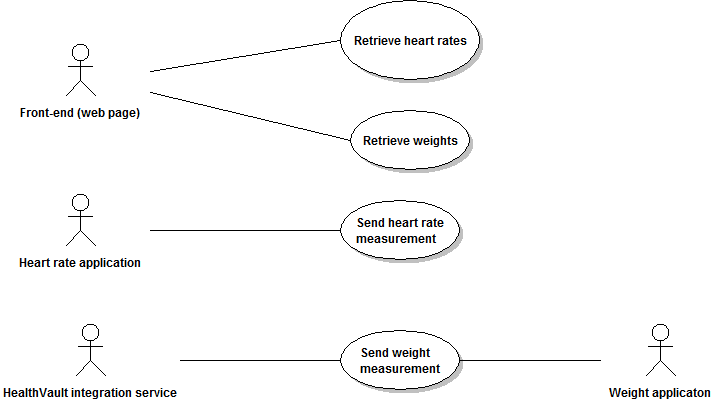
\includegraphics[scale=0.6]{../Figures/use-case-diagram-nipen.png}
\caption{Use case diagram - NIPEN}
\label{figure:use-case-diagram-nipen}
\end{figure}

In figure \ref{figure:use-case-diagram-nipen-front-end} a use case diagram is given for retrieving values from NIPEN.
Table \ref{table:use-case-retrieve-heart-rate-weight} gives a textual use case diagram for retrieval of the data values.

\begin{figure}[H]
\centering
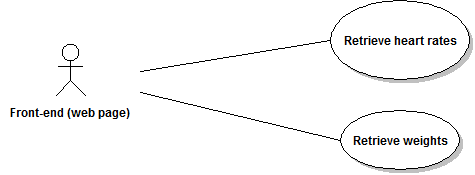
\includegraphics[scale=0.6]{../Figures/use-case-diagram-nipen-front-end.png}
\caption{Use case diagram - Retrieving values from NIPEN}
\label{figure:use-case-diagram-nipen-front-end}
\end{figure}

\begin{table}[H]
\begin{center}
\begin{tabular}{ l | p{10cm} }
  \hline
  \textbf{Use Case Element} & \textbf{Description} \\ \hline\hline
  Requirements & \hyperref[table:reqip]{FIP3} and \hyperref[table:reqip]{FIP4}\\ \hline
  Application & NIPEN \\ \hline
  Name & Retrieve data from NIPEN \\ \hline
  Description & Front-end retrieving heart rate and weight measurements from NIPEN. \\ \hline
  Actor & Front-end \\ \hline
  Precondition &
	\par 1. Multiple weight and heart rate measurements are stored on NIPEN.
	\\ \hline
  Basic Flow & 
  	\par 1. The front-end makes and API call to the front-end to receive heart rate measurements.
  	\par 2. The system sends the heart rate measurements as JSON models to the front-end. 
  	\par 3. The front-end makes and API call to the front-end to receive weight measurements.
  	\par 4. The system sends the weight measurements as JSON models to the front-end.
  	\\ \hline
\end{tabular}
\end{center}
\caption{Textual use case - Retrieve heart rate and weight measurements}
\label{table:use-case-retrieve-heart-rate-weight}
\end{table}

A use case diagram for retrieval of heart rate values at NIPEN is given in figure \ref{figure:use-case-diagram-nipen-heart-rate}.
The table below (table \ref{table:use-case-receive-heart-rate}) shows a textual use case for a scenario where NIPEN receives a heart rate measurement.

\begin{figure}[H]
\centering
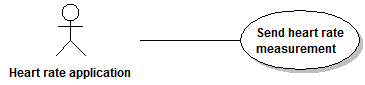
\includegraphics[scale=0.6]{../Figures/use-case-diagram-nipen-heart-rate.png}
\caption{Use case diagram - Receiving heart rate measurements at NIPEN}
\label{figure:use-case-diagram-nipen-heart-rate}
\end{figure}

\begin{table}[H]
\begin{center}
\begin{tabular}{ l | p{10cm} }
  \hline
  \textbf{Use Case Element} & \textbf{Description} \\ \hline\hline
  Requirements & \hyperref[table:reqip]{FIP1} \\ \hline
  Application & NIPEN \\ \hline
  Name & Receiving heart rate measurement \\ \hline
  Description & Receiving a heart rate measurement at NIPEN from the heart rate application. \\ \hline
  Actor & Heart Rate Application \\ \hline
  Basic Flow & 
  	\par 1. Heart rate application sends a heart rate measurement to NIPEN.
  	\par 2. NIPEN receives the heart rate measurement.
  	\par 3. NIPEN stores the values.
  	\\ \hline
\end{tabular}
\end{center}
\caption{Textual use case - Receiving a heart rate measurement at NIPEN}
\label{table:use-case-receive-heart-rate}
\end{table}

The use case diagram below (figure \ref{figure:use-case-diagram-nipen-weight}) shows NIPEN receiving weight values from the weight application and HealthVault integration service.
Table \ref{table:use-case-receive-weight} gives a textual use case for when NIPEN receives values from the weight applications. 

\begin{figure}[H]
\centering
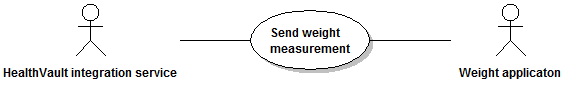
\includegraphics[scale=0.6]{../Figures/use-case-diagram-nipen-weight.png}
\caption{Use case diagram - Receiving weight measurements at NIPEN}
\label{figure:use-case-diagram-nipen-weight}
\end{figure}

\begin{table}[H]
\begin{center}
\begin{tabular}{ l | p{10cm} }
  \hline
  \textbf{Use Case Element} & \textbf{Description} \\ \hline\hline
  Requirements & \hyperref[table:reqip]{FIP2} \\ \hline
  Application & NIPEN \\ \hline
  Name & Receiving weight measurement \\ \hline
  Description & Receiving a weight measurement at NIPEN from the weight application and HealthVault integration service. \\ \hline
  Actor & Weight Application and HealthVault Integration Service \\ \hline
  Basic Flow & 
  	\par 1. Weight application sends a weight measurement to NIPEN.
  	\par 2. NIPEN receives the weight measurement.
  	\par 3. NIPEN stores the values.
  	\par 4. HealthVault integration platform sends a weight measurement to NIPEN.
  	\par 5. NIPEN receives the weight measurement.
  	\par 6. NIPEN stores the values.
  	\\ \hline
\end{tabular}
\end{center}
\caption{Textual use case - Receiving weight measurements at NIPEN}
\label{table:use-case-receive-weight}
\end{table}


\subsection{Front-end}

The use case diagram for the front-end is shown in figure \ref{figure:use-case-diagram-front-end}.
From the use case diagram we see that the front-end has two main objectives.
The first one is to fetch data from our integration platform, and the second one is to display this data to the user.
In table \ref{table:use-case-view-data} we present a textual use case for the front-end.

\begin{figure}[H]
\centering
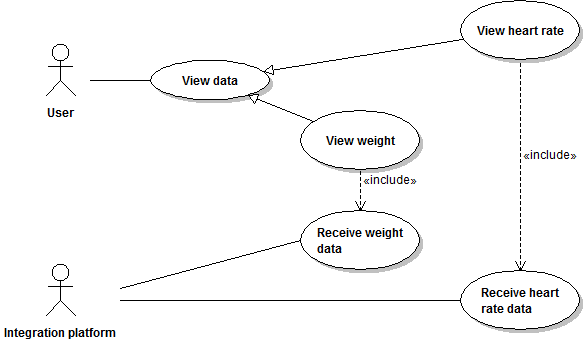
\includegraphics[scale=0.6]{../Figures/use-case-diagram-front-end.png}
\caption{Use case diagram - Front-end}
\label{figure:use-case-diagram-front-end}
\end{figure}

\begin{table}[H]
\begin{center}
\begin{tabular}{ l | p{10cm} }
  \hline
  \textbf{Use Case Element} & \textbf{Description} \\ \hline\hline
  Requirements & \hyperref[table:reqfrontend]{FW1}, \hyperref[table:reqip]{FIP3} and \hyperref[table:reqip]{FIP4}\\ \hline
  Application & Front-end \\ \hline
  Name & View data \\ \hline
  Description & Display the data from NIPEN for the user. \\ \hline
  Actor & User and NIPEN \\ \hline
  Precondition &
	\par 1. NIPEN has data about the current user.
	\par 2. NIPEN is online.
	\par 3. The user is using a computer with a web browser, that is connected to the internet.
	\\ \hline
  Basic Flow & 
  	\par 1. The user accesses the web page.
  	\par 2. Front-end requests data from NIPEN.
  	\par 3. NIPEN sends data to front-end.
  	\par 4. Front-end displays data to user.
  	\\ \hline
  Alternate Flows & 
  	\par 1A: The user wants to only view heart rate data.
  	\par\hspace{15pt} 1. The user clicks on \textit{Heart Rate} in the navigation bar.
  	\par 1B: The user wants to only view weight data.
  	\par\hspace{15pt} 1. The user clicks on \textit{Weight} in the navigation bar.
  \\ \hline
\end{tabular}
\end{center}
\caption{Textual use case - View data}
\label{table:use-case-view-data}
\end{table}

\subsection{Heart Rate Application}

A use case diagram for the heart rate application is presented in figure \ref{figure:use-case-diagram-heart-rate}.
The main objectives of this application is to measure and send the data to the integration platform.

\begin{figure}[H]
\centering
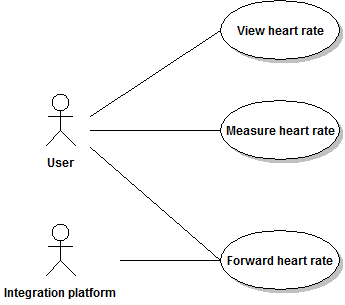
\includegraphics[scale=0.6]{../Figures/use-case-diagram-heart-rate.png}
\caption{Use case diagram - Heart rate application}
\label{figure:use-case-diagram-heart-rate}
\end{figure}

A textual use case for measuring and viewing the heart rate is presented in table \ref{table:use-case-measure-heart-rate}.
Figure \ref{figure:use-case-diagram-measure-heart-rate} shows a use case diagram for the textual use case.

\begin{figure}[H]
\centering
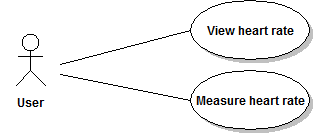
\includegraphics[scale=0.75]{../Figures/use-case-diagram-measure-and-view-heart-rate.png}
\caption{Use case diagram - Measure and view heart rate}
\label{figure:use-case-diagram-measure-heart-rate}
\end{figure}

\begin{table}[H]
\begin{center}
\begin{tabular}{ l | p{10cm} }
  \hline
  \textbf{Use Case Element} & \textbf{Description} \\ \hline\hline
  Requirements & \hyperref[table:reqheartrate]{FHR1} and \hyperref[table:reqheartrate]{FHR2} \\ \hline
  Application & Heart Rate Application \\ \hline
  Name & Measure and view heart rate \\ \hline
  Description & Measure the heart rate of the user and then view the measured data. \\ \hline
  Actor & User \\ \hline
  Precondition &
    \par 1. The users phone meets the requirements of the heart rate application.
  	\par 2. The application is installed on the users phone.
  	\par 3. The application is running on the users phone.
  \\ \hline
  Basic Flow & 
  	\par 1. The user places his finger on the camera of the phone.
  	\par 2. The user waits until the heart rate is shown on the display.
  	\par 3. The user views the heart rate.
  \\ \hline
  Alternate Flows & 
  	\par 1A: The user places his finger wrongly, which makes the measured data incorrect.
  	\par\hspace{15pt} 1. The user adjusts his finger.
  \\ \hline
\end{tabular}
\end{center}
\caption{Textual use case - Measure and view heart rate}
\label{table:use-case-measure-heart-rate}
\end{table}

Table \ref{table:use-case-send-heart-rate} presents a textual use case for sending the heart rate measurementes to
the integration platform. Figure \ref{figure:use-case-diagram-send-heart-rate} shows a use case diagram for the textual use case.

\begin{figure}[H]
\centering
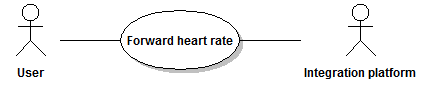
\includegraphics[scale=0.75]{../Figures/use-case-diagram-send-heart-rate.png}
\caption{Use case diagram - Send heart rate}
\label{figure:use-case-diagram-send-heart-rate}
\end{figure}

\begin{table}[H]
\begin{center}
\begin{tabular}{ l | p{10cm} }
  \hline
  \textbf{Use Case Element} & \textbf{Description} \\ \hline\hline
  Requirements & \hyperref[table:reqheartrate]{FHR3} and \hyperref[table:reqip]{FIP1} \\ \hline
  Application & Heart Rate Application \\ \hline
  Name & Send heart rate \\ \hline
  Description & Send the measured heart rate to the integration platform. \\ \hline
  Actor & User and NIPEN \\ \hline
  Precondition &
    \par 1. The user has measured his/hers heart rate through the application.
    \par 2. The phone is connected to the internet.
    \par 3. NIPEN is online.
  \\ \hline
  Basic Flow & 
  	\par 1. The user clicks on \textit{Send}.
  	\par 2. The application sends the data to the NIPEN.
  	\par 3. NIPEN receives the data.
  \\ \hline
\end{tabular}
\end{center}
\caption{Textual use case - Send heart rate}
\label{table:use-case-send-heart-rate}
\end{table}

\subsection{Weight Application}

The goal of the weight application is to retrieve weight data from HaulthVault.
It should also be able to send weight measurements to our integration platform.
Figure \ref{figure:use-case-diagram-weight} shows the main use case diagram for the application.

\begin{figure}[H]
\centering
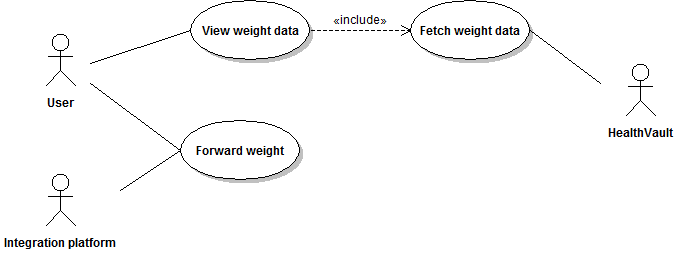
\includegraphics[scale=0.6]{../Figures/use-case-diagram-weight.png}
\caption{Use case diagram - Weight application}
\label{figure:use-case-diagram-weight}
\end{figure}

Figure \ref{figure:use-case-diagram-view-weight} shows a use case diagram for fetching and viewing the weight data.
Table \ref{table:use-case-view-weight-data} gives a textual use case for the use case diagram.

\begin{figure}[H]
\centering
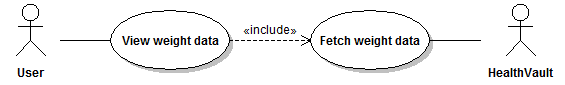
\includegraphics[scale=0.75]{../Figures/use-case-diagram-view-weight.png}
\caption{Use case diagram - View weight data}
\label{figure:use-case-diagram-view-weight}
\end{figure}

\begin{table}[H]
\begin{center}
\begin{tabular}{ l | p{10cm} }
  \hline
  \textbf{Use Case Element} & \textbf{Description} \\ \hline\hline
  Requirements & \hyperref[table:reqweight]{FHV1} and \hyperref[table:reqweight]{FHV2}\\ \hline
  Application & Weight Application \\ \hline
  Name & View weight data \\ \hline
  Description & Fetch the weight data from HealthVault and display it for the user. \\ \hline
  Actor & User and HealthVault \\ \hline
  Precondition &
    \par 1. The users phone meets the requirements of the weight application.
  	\par 2. The application is installed on the users phone.
  	\par 3. The application is running on the users phone.
  	\par 4. The application is connected to the internet.
  \\ \hline
  Basic Flow & 
  	\par 1. The user writes his email to HealthVault into the email field.
  	\par 2. The user writes his password to HealthVault into the password field.
  	\par 3. The user clicks on a button to login.
  	\par 4. The application shows the data for the user.
  	\par 5. The user views the data.
  \\ \hline
  Alternate Flows & 
  	\par 3A: The user inputs an invalid password or email.
  	\par\hspace{15pt} 1. The user has to go back to step 1 and start over again.
  \\ \hline
\end{tabular}
\end{center}
\caption{Textual use case - View weight data}
\label{table:use-case-view-weight-data}
\end{table}

Table \ref{table:use-case-send-weight-data} gives a textual use case for sending the weight data to our
integration platform. Figure \ref{figure:use-case-diagram-send-weight} displays a use case diagram for the
textual use case.

\begin{figure}[H]
\centering
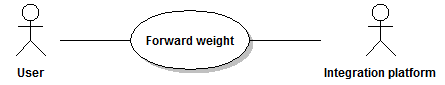
\includegraphics[scale=0.75]{../Figures/use-case-diagram-send-weight.png}
\caption{Use case diagram - Send weight data}
\label{figure:use-case-diagram-send-weight}
\end{figure}

\begin{table}[H]
\begin{center}
\begin{tabular}{ l | p{10cm} }
  \hline
  \textbf{Use Case Element} & \textbf{Description} \\ \hline\hline
  Requirements & \hyperref[table:reqweight]{FHV3} and \hyperref[table:reqip]{FIP2}\\ \hline
  Application & Weight Application \\ \hline
  Name & Send weight data \\ \hline
  Description & Send the weight data from the phone application into the integration platform. \\ \hline
  Actor & User and NIPEN \\ \hline
  Precondition &
    \par 1. NIPEN is online.
    \par 2. The user has logged in to HealthVault through the app.
  \\ \hline
  Basic Flow & 
    \par 1. The user enters a weight measurement into the weight field.
  	\par 2. The user presses the \textit{Send} button.
  	\par 3. NIPEN receives the data.
  \\ \hline
\end{tabular}
\end{center}
\caption{Textual use case - Send weight data}
\label{table:use-case-send-weight-data}
\end{table}

\subsection{HealthVault Integration Service}

The goal of the HealthVault Integration Service is to poll data regularly from HealthVault.
If a new value is detected then it is sent to the integration platform.
The web service should also be capable of sending weight values to HealthVault.
Figure \ref{figure:use-case-diagram-weight-service} shows a use case diagram of the system.

\begin{figure}[H]
\centering
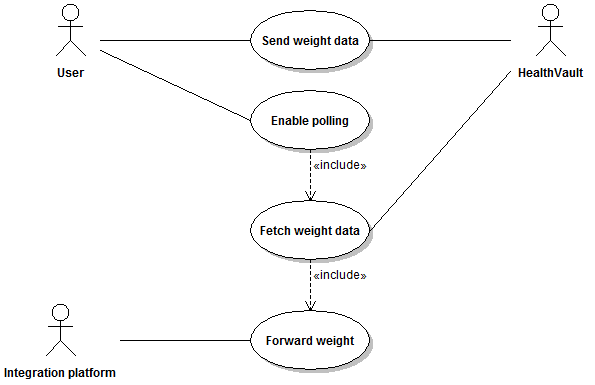
\includegraphics[scale=0.75]{../Figures/use-case-diagram-weight-service.png}
\caption{Use case diagram - HealthVault Integration Service}
\label{figure:use-case-diagram-weight-service}
\end{figure}

Figure \ref{figure:use-case-diagram-weight-service-send} shows a use case diagram for the sending functionality, while table \ref{table:use-case-send-weight-to-healthvault} gives a textual use case.

\begin{figure}[H]
\centering
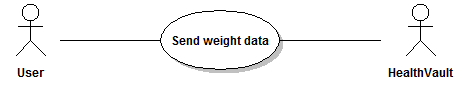
\includegraphics[scale=0.75]{../Figures/use-case-diagram-weight-service-send.png}
\caption{Use case diagram - HealthVault Integration Service send to HealthVault}
\label{figure:use-case-diagram-weight-service-send}
\end{figure}

\begin{table}[H]
\begin{center}
\begin{tabular}{ l | p{10cm} }
  \hline
  \textbf{Use Case Element} & \textbf{Description} \\ \hline\hline
  Requirements & \hyperref[table:reqwebservice]{FHIS3}\\ \hline
  Application & HealthVault Integration Service \\ \hline
  Name & Send weight to HealthVault \\ \hline
  Description & Send a weight measurement from the web service into HealthVault. \\ \hline
  Actor & User and HealthVault\\ \hline
  Precondition &
    \par 1. The user has logged in to HealthVault through the web service.
  \\ \hline
  Basic Flow & 
  	\par 1. The user enters a weight value into the weight field.
  	\par 2. User clicks on the send button.
  	\par 3. HealthVault receives the data.
  \\ \hline
\end{tabular}
\end{center}
\caption{Textual use case - Send weight to HealthVault}
\label{table:use-case-send-weight-to-healthvault}
\end{table}

In figure \ref{figure:use-case-diagram-weight-service-poll} an overview is given of the polling service.
Table \ref{table:use-case-start-polling-service} shows a textual use case for the polling functionality.

\begin{figure}[H]
\centering
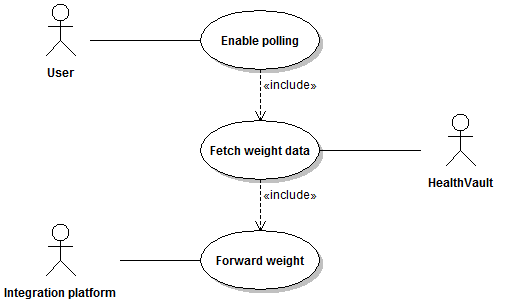
\includegraphics[scale=0.75]{../Figures/use-case-diagram-weight-service-poll.png}
\caption{Use case diagram - HealthVault Integration Service data polling}
\label{figure:use-case-diagram-weight-service-poll}
\end{figure}

\begin{table}[H]
\begin{center}
\begin{tabular}{ l | p{10cm} }
  \hline
  \textbf{Use Case Element} & \textbf{Description} \\ \hline\hline
  Requirements & \hyperref[table:reqwebservice]{FHIS1}, \hyperref[table:reqwebservice]{FHIS2} and \hyperref[table:reqip]{FIP2}\\ \hline
  Application & HealthVault Integration Service \\ \hline
  Name & Start polling service \\ \hline
  Description & Start the polling service and send data from HealthVault to the integration platform. \\ \hline
  Actor & User, HealthVault and NIPEN \\ \hline
  Precondition &
    \par 1. The user has logged in to HealthVault through the web service.
    \par 2. The polling service is off.
  \\ \hline
  Basic Flow & 
  	\par 1. The user clicks on \textit{Enable} button to start the polling service.
  	\par 2. The web service polls data from HealthVault.
  	\par 3. The web service checks if new data is retrieved.
  \\ \hline
   Alternate Flows & 
  	\par 3A: No new weight measurement.
  	\par\hspace{15pt} 1. Go to 2 and poll again.
  	\par 3B: New weight measurement detected.
  	\par\hspace{15pt} 1. Send new weight data to NIPEN.
  	\par\hspace{15pt} 2. NIPEN receives data.
  	\par\hspace{15pt} 3. Go to 2 and poll again.
  \\ \hline
\end{tabular}
\end{center}
\caption{Textual use case - Start polling service}
\label{table:use-case-start-polling-service}
\end{table}

%\section{Test plan}
%\label{section:testplan}

%Most of the testing was performed manually.
%Since the product consisted of two Android applications and a Spring
 
\chapter{System architecture}
\label{ch:architecture}

\lhead{Chapter 5. \emph{System architecture}}

%In this chapter we are going to give a description of the system architecture.
This chapter describes the system architecure in detail.
We follow a top-down approach, giving an overview of the architecture and then detailing
each part in a separate section.
%We start this chapter with an overview, where we give an abstract description of our project.
%Then we are going to give a more thorough description of each of our applications.

\section{Overview}

%In order to study the possibilities of leveraging modern mobile phones in an integration platform
%we developed a product consisting of multiple, interoperable systems which include:
The product consists of multiple, interoperable systems including:% that communicate with each other.
%The applications are listed below:
\begin{enumerate}[1.]
	\item an integration platform (\textit{NIPEN})
	\item a front-end to the integration platform
	%\item an Android application to measure heart rate
	%\item an Android application to showcase HealthVault interoperability
	\item two Android applications
	\item a web service%to showcase HealthVault interoperability
\end{enumerate}

Figure \ref{figure:architecture} shows the overall system architecture.

In the following sections we provide a detailed description of the each part of the system.
%an abstract architecture is given of how our applications communicate with each other.

%%
\iffalse
%% we talk about this more in detail in other sections
NIPEN or NIP is our server application that consists of an API and a database.
This application is capable of receiving weight and heart rate data and store them in a database.
It is also able to retrieve data from the database and then send it to our front-end, which then visualizes
the information sent.
The next three applications are able to send information to NIP.
For instance the heart rate application is capable of measuring a heart rate and then send it to the integration platform.
The two last applications are able to fetch weight data from HealthVault and send it to NIP.
The main difference between them is that the \textit{Weigh Application} runs on an Android device, while the
\textit{HealthVault Integration Service} runs on a server or a computer.
\fi

\iffalse
% * these are some limitations to our product. should we have a separate section maybe in the conclusion for these? *
We didn't want to make our applications to complicated, duo to time restriction and lack of resources.
Thus we have only concentrated on one user.
What this means is that we have not implemented functionality for storing and displaying data for multiple users.
However our data structures and database tables support more than one user, since they all contain a user ID.
We have however not implemented any logic to handle several users, this was after all not a requirement.
In addition our systems doesn't contain any type of security, i.e. no authentication or data encryption.
The reason for this is that our customer was explicit that security was not a requirement.
Also, our applications are meant to be a prototype to illustrate how a system like this would work.
And hence security is not necessary.
\fi

\section{Rationale}

\begin{figure}[h]
\centering
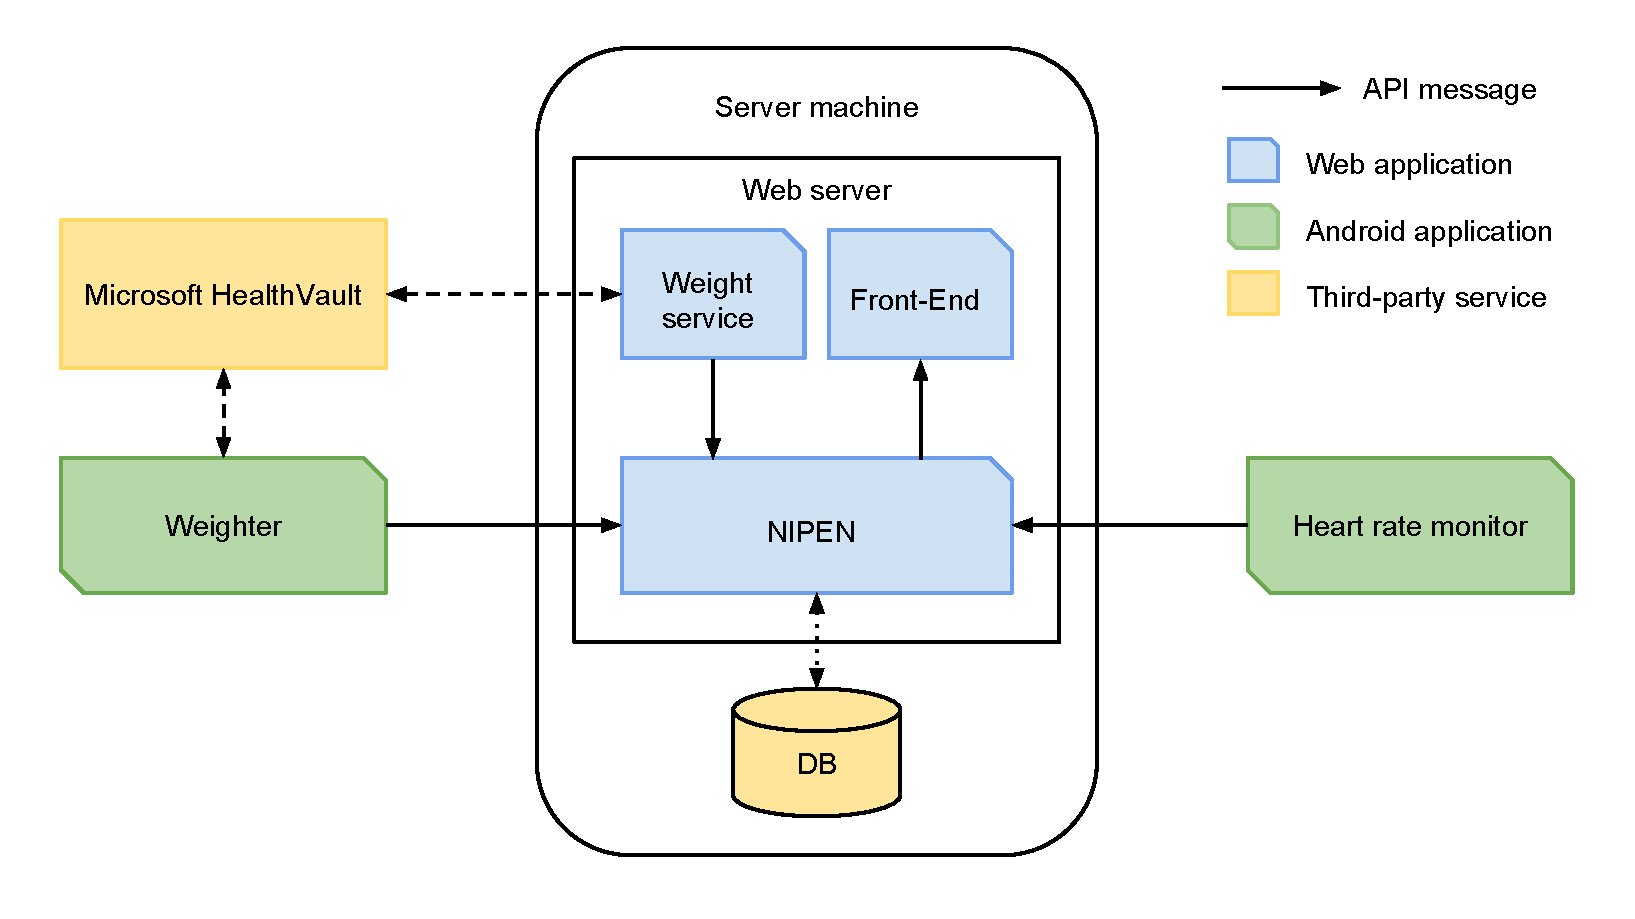
\includegraphics[scale=0.5]{../Figures/architecture.pdf}
\caption{System architecture}
\label{figure:architecture}
\end{figure}

\section{NIPEN}

NIPEN is the core of our product. It is an implementation of a web API for the storage and retrieval of health information.
%To provide such functionality, we had to define a \textit{model} (a representation) of the information itself.
Together with the customer, we identified two types of health measurements that would be supported by NIPEN:
heart rate and weight. %why heartrate and weight?
%This choice was motivated by the fact that both are easy to obtain using mobile phones. what about weight?
For each of these measurements we designed a \textit{model}, that is a digital representation of the information,
which we describe in detail subsection \ref{subsec:models}.
NIPEN is exposing an API that other applications can use to interoperate with it.
The API is presented in subsection \ref{subsec:api}.

%NIPEN is an integration platform for two data types, namely heart rate and weight measurements.
%By using the HTTP methods GET and POST it is possible to retrieve and store data into NIP, respectively.
%The following subsection provides a more detailed explaination of how we achieved that.
%How this works is explained in this subsection.

\subsection{Architectural pattern}

A class diagram containing the most important classes and methods of our system is given
in figure \ref{figure:nipen-class-diagram}.

\begin{figure}[h]
\centering
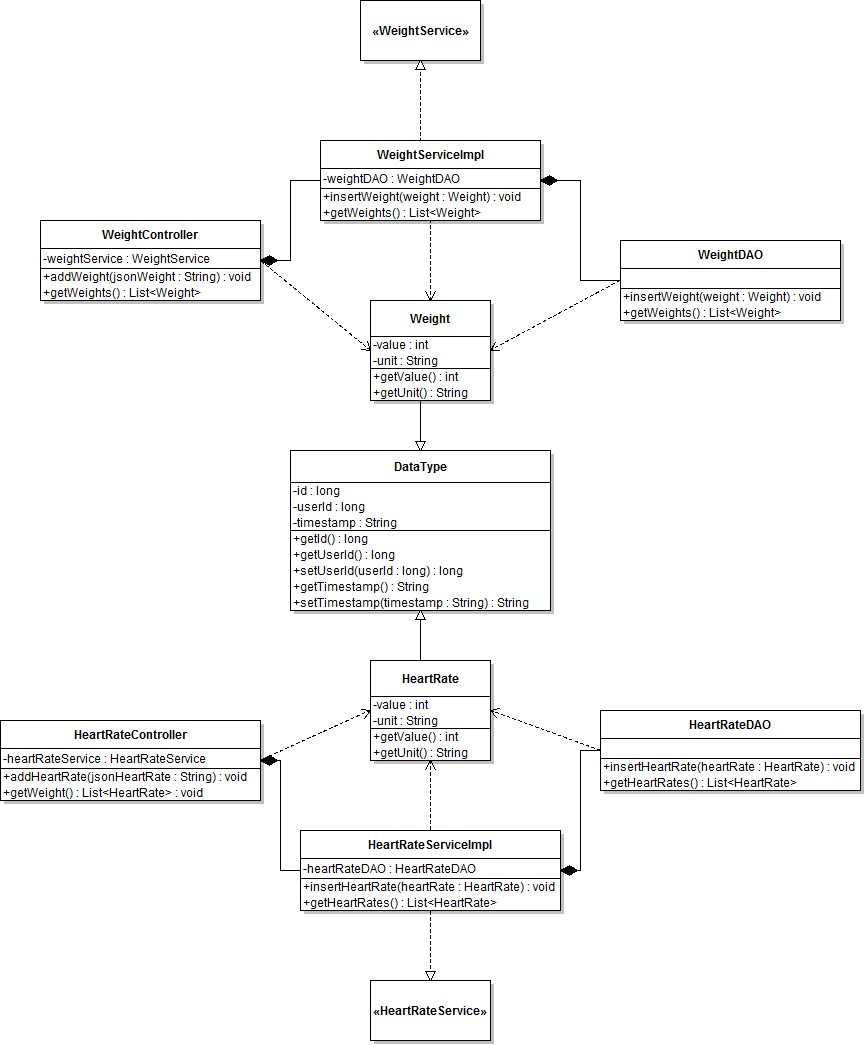
\includegraphics[scale=0.5]{../Figures/NIPEN-class-diagram.png}
\caption{NIPEN class diagram}
\label{figure:nipen-class-diagram}
\end{figure}

We are following an MVC (Model-View-Controller) architectural pattern. %% WHY ?
What this means is that we have divided our application into three main parts: models, views and controllers.

\begin{itemize}

\item Model: A model is \iffalse a type of\fi a data structure that is used within an application.
In our case the models of our application are: Weight and HeartRate.
%and DataType. sure but it is just an abstract superclass
This classes are filled with data from the database and are used when sending data to the front-end.
They are also used to store data into our database.

\item View: A view is something that displays the data from the models to the users.
The front-end is the view in our case.
How the front-end works is described in subsection \ref{subsec:front-end}.

\item Controller: The controller is responsible for updating the models that are going to be used in the view.
In our application the controllers are called when a HTTP GET or HTTP POST request is sent to a specific URL.
The controllers work as an interface that connects the applications we have developed with our back-end.

\end{itemize}

\subsection{Data models}
\label{subsec:models}

We decided to represent our data models using JSON.
Although there were other perfectly viable alternatives like XML,
we opted for JSON because it is less verbose and we had previous experiences with it.
Additionally, JSON APIs are used by major networking services which deal with huge amounts of
data like Facebook and Twitter.
%We are using JSON strings when transmitting data to and from the server.
%The representation of the data is inspired from the Human API.
human/api, described in section \ref{section:humanapi}, provided a good starting point for the design of
these models which we have simplified and adapted to our needs.
Both heart rate and weight measurements have \iffalse are represented with\fi the same attributes.
This is due to the fact that their are rather simple measurements which involve nothing more but
a user's ID, a value, a unit, and a timestamp.
%They contain an ID, user ID, timestamp, value and a unit.
%The ID is not needed, when the JSON string is sent, because it is created on the server side.
%Below is a representation of a heart rate JSON string that can be used to store heart rate data on the server:
See below an example of JSON model for heart rate measurements.

\begin{lstlisting}[language=json]
{
	"userId":1,
	"timestamp":"2013-10-27 14:57:39.0",
	"value":75,
	"unit":"bpm"
}
\end{lstlisting}

A weight model looks pretty much the same (see below), but uses another unit.
%The ID of the data is shown when receiving the data from the server:

\begin{lstlisting}[language=json]
{
	"userId":1,
	"timestamp":"2013-10-27 14:57:39.0",
	"value":90,
	"unit":"kg"
}
\end{lstlisting} 

\subsection{Web API}
\label{subsec:api}

% are we actually using REST?
% we don't have PUT and DELETE methods, also our entry points are wrong from a REST perspective: different urls
%A RESTful (Representational State Transfer) service is used when communicating with NIPEN.
NIPEN exposes a JSON based web API to store and retrieve health information.
% which other applications can use to interoperate.
By using a web API, we ensure that the system is accessible to a broad number of users an from a wide
selection of devices. All that is needed is an internet connection.
In fact, the API is exposed to the web via a web server, in this case Apache Tomcat 7.
There were of course a number of alternative web servers we could have used but we sticked
with Tomcat because we had used it before and it provided all needed functionality.
Applications can interact with NIPEN by issuing HTTP GET and POST messages to pre-defined URLs
% to retrieve or store
%heart rate and weight data models.
called API endpoints.
Internally, these methods are handled by Spring \textit{Controllers} which implement the logic of the API.
Each API endpoint is associated with a resource and an action to be perfomed on it as shown in table \ref{table:api}.
%What this means is that we are using HTTP methods to request and send data.
%We have two controllers that handle the API calls, concerning the heart rate and weight data, in our system.
%They are called \textit{HeartRateController} and \textit{WeightController}. 
%The \textit{HeartRateController} controls retrieval and storage of heart rate, while 
%the \textit{WeightController} handles weight data.
%These controllers handle two HTTP methods, POST for pushing data and GET for retrieving data.
%When requesting data from our API an HTTP GET request needs to be performed to one of the following URLs:

\begin{table}[h]
\begin{center}
\begin{tabular}{ | l | l | c | c | }
	\hline
	Resource	& URL						& HTTP Method 	& Action \\
	\hline
	Heart rate	& /nipen/api/heart\_rates	& GET			& Read \\
	Weight		& /nipen/api/weights		& GET			& Read \\
	Heart rate	& /nipen/api/heart\_rate	& POST			& Write \\
	Weight		& /nipen/api/weight			& POST			& Write \\
	\hline
\end{tabular}
\end{center}
\caption{API endpoints}
\label{table:api}
\end{table}

%% reworked the endpoints into a single table.
\iffalse
\begin{itemize}
\item $<$server address$>$/nipen/api/human/heart\_rates
\item $<$server address$>$/nipen/api/human/weights
\end{itemize}

The first URL requests all the heart rates, while the second URL requests all the weights stored in the database.
In figure \ref{figure:retrieve-heart-rates-from-the-database} a sequence diagram is given of how the controller 
retrieves the data for the user.
The weight controller works the same way.
%% maybe too detailed here
When the controller receives a HTTP GET request, it contacts a data type service which again contacts a
database handler class.
The database handler class returns a list of models which is at last returned to the controller.
The list of models is transformed automatically into JSON string with help of the Spring Framework.
Both controllers will respond with an array of JSON strings representing the respective data.
\fi

When an application makes an HTTP GET request at the URL \verb|/nipen/api/heart_rates| it is returned
a JSON string representing a collection (array) of all heart rate measurements stored in the database.
See below for an example:
\begin{lstlisting}[language=json]
[
	{
		"id":319,
		"userId":1,
		"timestamp":"2013-10-21 07:35:32.0",
		"value":70,
		"unit":"bpm"
	},
	{
		"id":320,
		"userId":1,
		"timestamp":
		"2013-10-22 17:53:09.0",
		"value":66,
		"unit":"bpm"
	}
]
\end{lstlisting}
\label{listing:jsonarray}

Similarly, the application is returned a collection of all weight measurements when making an HTTP GET
request at: \verb|/nipen/api/weights|. Figure \ref{figure:seqhr} shows
a sequence diagram for retrieving heart rates.

\begin{figure}[h]
\centering
%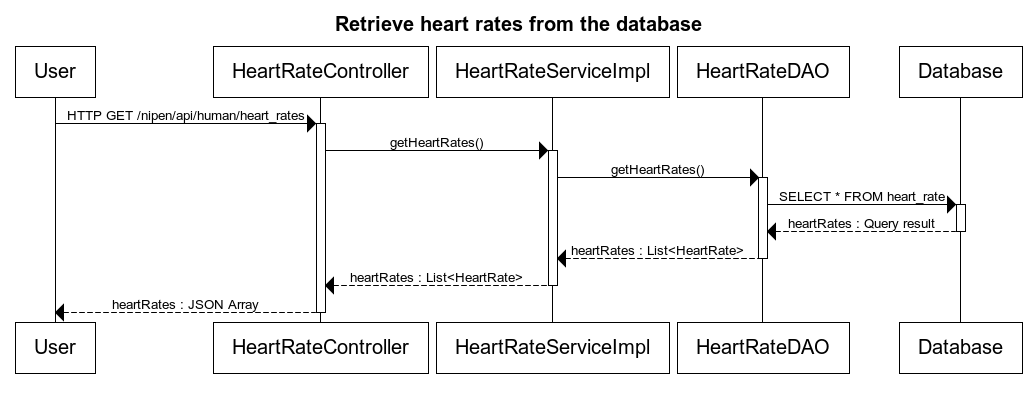
\includegraphics[scale=0.6]{../Figures/retrieve-heart-rates-from-the-database.png}
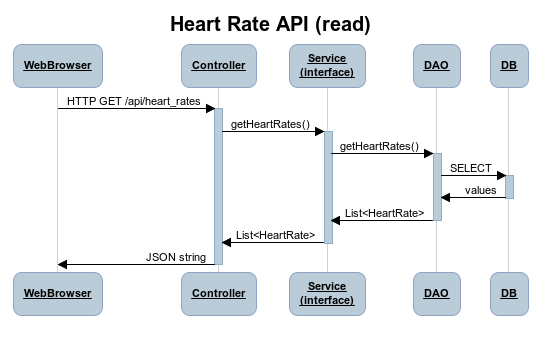
\includegraphics[scale=0.8]{../Figures/seqhr.png}
\caption{Retrieving heart rates from the database}
\label{figure:seqhr}
\end{figure}

When an HTTP POST operation is performed on either \verb|/nipen/api/weight| or \newline
\verb|/nipen/api/heart_rate| then the JSON payload will be translated into a MVC model and
stored into the database. See figure \ref{figure:seqw} for a sequence diagram.

\iffalse
\begin{itemize}
\item $<$server address$>$/nipen/api/human/heart\_rate
\item $<$server address$>$/nipen/api/human/weight
\end{itemize}

With the POST method a JSON string with the specified data type needs to be sent. 
How the controller handles this message is shown in figure \ref{figure:pushing-weight-into-NIPEN}.
The diagram shows an example of how to push a weight value into NIPEN.
The application works the same way when pushing a heart rate value into the system.
When the application receives the JSON string, it first needs to parse it into its respective model class.
After that it is sent to a service class which then sends it to a database handler class.
This class stores the value into the database.
\fi

\begin{figure}[h]
\centering
%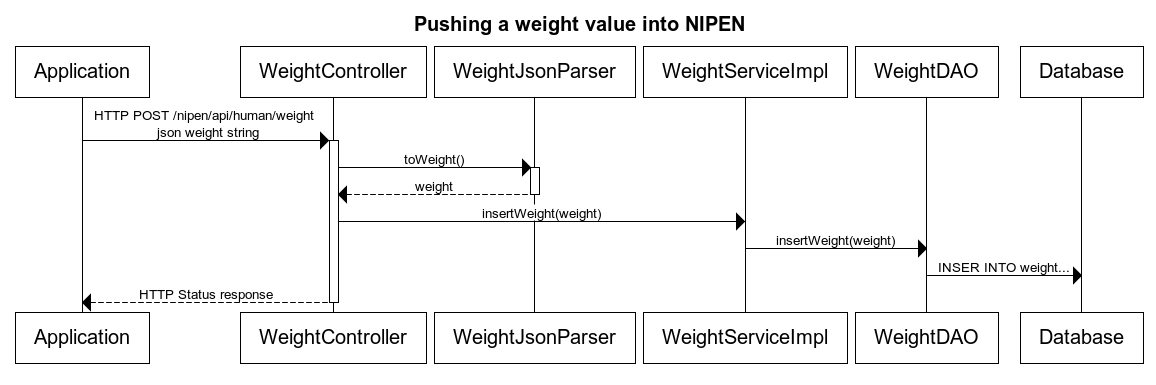
\includegraphics[scale=0.55]{../Figures/pushing-weight-into-NIPEN.png}
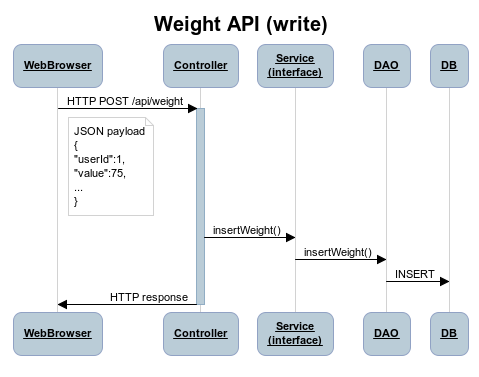
\includegraphics[scale=0.8]{../Figures/seqw.png}
\caption{Pushing a weight value into NIPEN}
\label{figure:seqw}
\end{figure}


\subsection{Database}

In order to implement persistency of health information we are using a MySQL database.
Although there were some alternative database implementations we opted for MySQL
because we were familiar with it and it offered all the features we needed.
%We are using a MySQL database for data storage.
The whole database is very simple and consists of two tables only: one for each supported health measurement.
%one for heart rate and one for weight.
%The heart rate table is shown in figure \ref{figure:heart-rate-database-diagram}
%and the weight table in figure \ref{figure:weight-database-diagram}.
The tables are shown in figure \ref{figure:heart-rate-database-diagram} (heart rate)
and \ref{figure:weight-database-diagram} (weight).
Although the tables are identical, we didn't want to merge them because it would 
have been a bad idea generally, making queries more expensive on large amounts of data.

%As we can see the tables are identical, the only difference is the name.
%The reason we didn't merge this tables is to separate the data, and it is also more efficient.
%It would require more resources to separate the data if they all were in one table.

\begin{figure}[h]
\centering
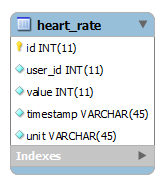
\includegraphics[scale=1.0]{../Figures/heart-rate-database-diagram.png}
\caption{Heart rate database diagram}
\label{figure:heart-rate-database-diagram}
\end{figure}

\begin{figure}[h]
\centering
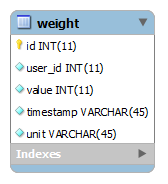
\includegraphics[scale=1.0]{../Figures/weight-database-diagram.png}
\caption{Weight database diagram}
\label{figure:weight-database-diagram}
\end{figure}

Access to the database in NIPEN is implemented by two classes: HeartRateDAO and WeightDAO.
Both provide functionality to read and write entries from/to the respective table in the database.
Having only one access point to the database is generally a good practice because it permits to
identify errors more easily as they can only be in one place.
%We have created separate classes for accessing the database through our server application.
%One for heart rate (HeartRateDAO) and one for weight (WeightDAO).
%This two classes contain a method for inserting and a method for fetching data from the database.
The data that is fetched from the database is ordered by timestamp, so that other applications
don't have to sort it themselves.
%In this way the other parts of the system doesn't need to sort the data afterwards.

%------


\section{Front-end}
\label{subsec:front-end}

The main functionality of the front-end is to visualize the data stored by NIPEN.%the Integration Platform.
This is accomplished by using a regular web-page consisting of HTML, CSS and JavaScript. HTML and CSS are used for structuring and giving a nice design to the web page. With help of JavaScript we are able to make the page dynamic.

\subsection{Design and Visualization}

One of the requirements given by the customer was that the front-end should use helsenorge.no color palette
(see figure \ref{figure:helsenorge-color-palette}).
%That is the front-end should use the colors shown in figure \ref{figure:helsenorge-color-palette}.
The front-end should show how helsenorge.no could represent the data from the integration platform. 
Since it would somehow mimic that page, we though that our web page should look similar to helsenorge.no. 
Hence we didn't only use the colors from the given palette, but tried as well to create a similar structure.

\begin{figure}[h]
\centering
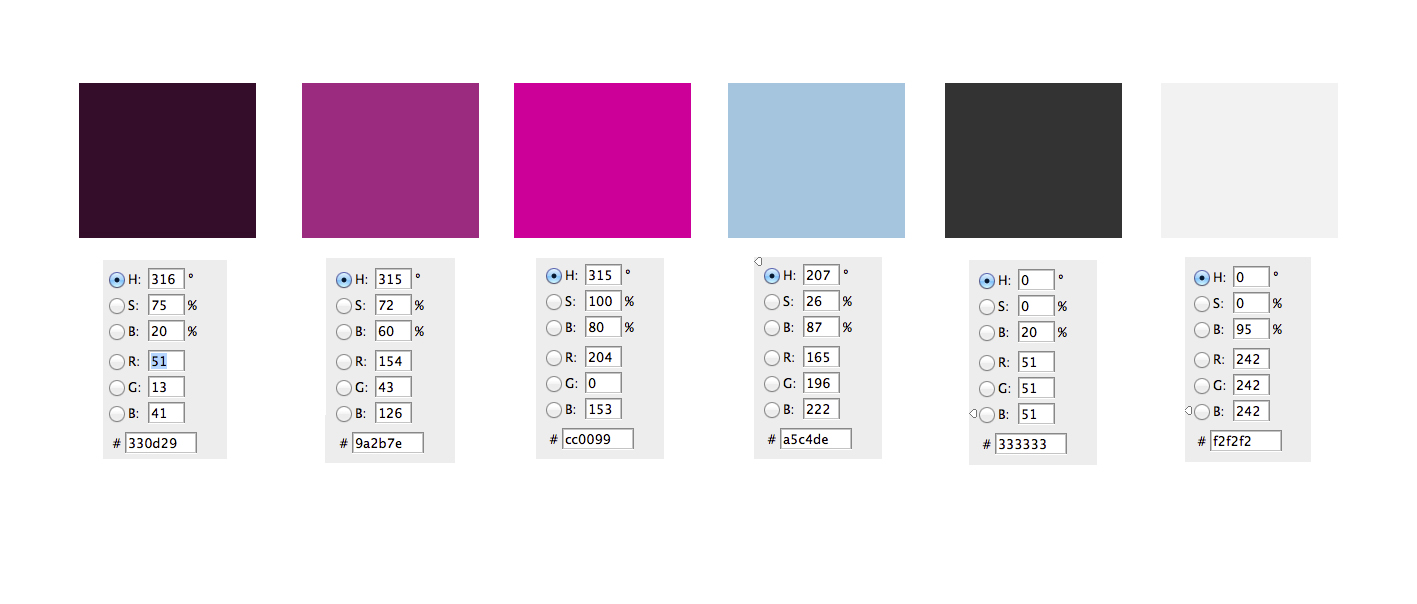
\includegraphics[scale=0.30]{../Figures/helsenorge_pallett.jpg}
\caption{Helsenorge color palette}
\label{figure:helsenorge-color-palette}
\end{figure}

We wanted to keep our front-end simple and user friendly.
%% again shall we mention this in a Limitations section in the conclusion maybe?
%, and since this is only a prototype are we only focusing on one user.
%hence we are only concentrating on how the web page should look like if the user is logged in. 
%Therefore we didn't create any authentication page and thus the user doesn't need to log in. 
%% you say this twice
%The front-end simply consists of one HTML file with some CSS and script files.
Twitter Bootstrap was used as a template to get started with the front-end development.
With help of JavaScript combined with jQuery, were we able to have three web pages in one HTML file. 
The main page \iffalse consists of\fi shows two graphs, one for heart rate and one for weight measurements. 
A visualization of the two latest values measured for each data type is also shown on the left side of the chart.
%Then we have two separate pages for heart rate and for weight.
Charts can also be visualized singularly on separate pages, where they can make use of some more space.
%These pages consists of an enlarged graph of the given data type being viewed.

%%
%This is simply accomplished by hiding the elements that are not used on those pages, and scaling the respective
%graph so it becomes larger.
With help of jQuery it's not a difficult task.
As a bonus jQuery is able to give an animation when hiding, showing and scaling the elements.
This is a nice touch to the web page.

We used a JavaScript library called Chart.js to display health measurements as charts. 
%With help of this library we are able to display the heart rates and weights as bar charts.
This library also has some animations when the graphs are created.
In our application a restriction is given to only display the 10 last measurements in the graphs.
If we have more than that the timestamp of the measurements becomes hard to read.

Figures \ref{figure:frontend-main-page}, \ref{figure:frontend-heart-rate-page} and \ref{figure:frontend-weight-page}
show various pages of the frontend.
%How the web-pages look like is shown in figure \ref{figure:frontend-main-page}, \ref{figure:frontend-heart-rate-page} and \ref{figure:frontend-weight-page}.

%%%% maybe they are too many and too similar?

\begin{figure}[H]
\centering
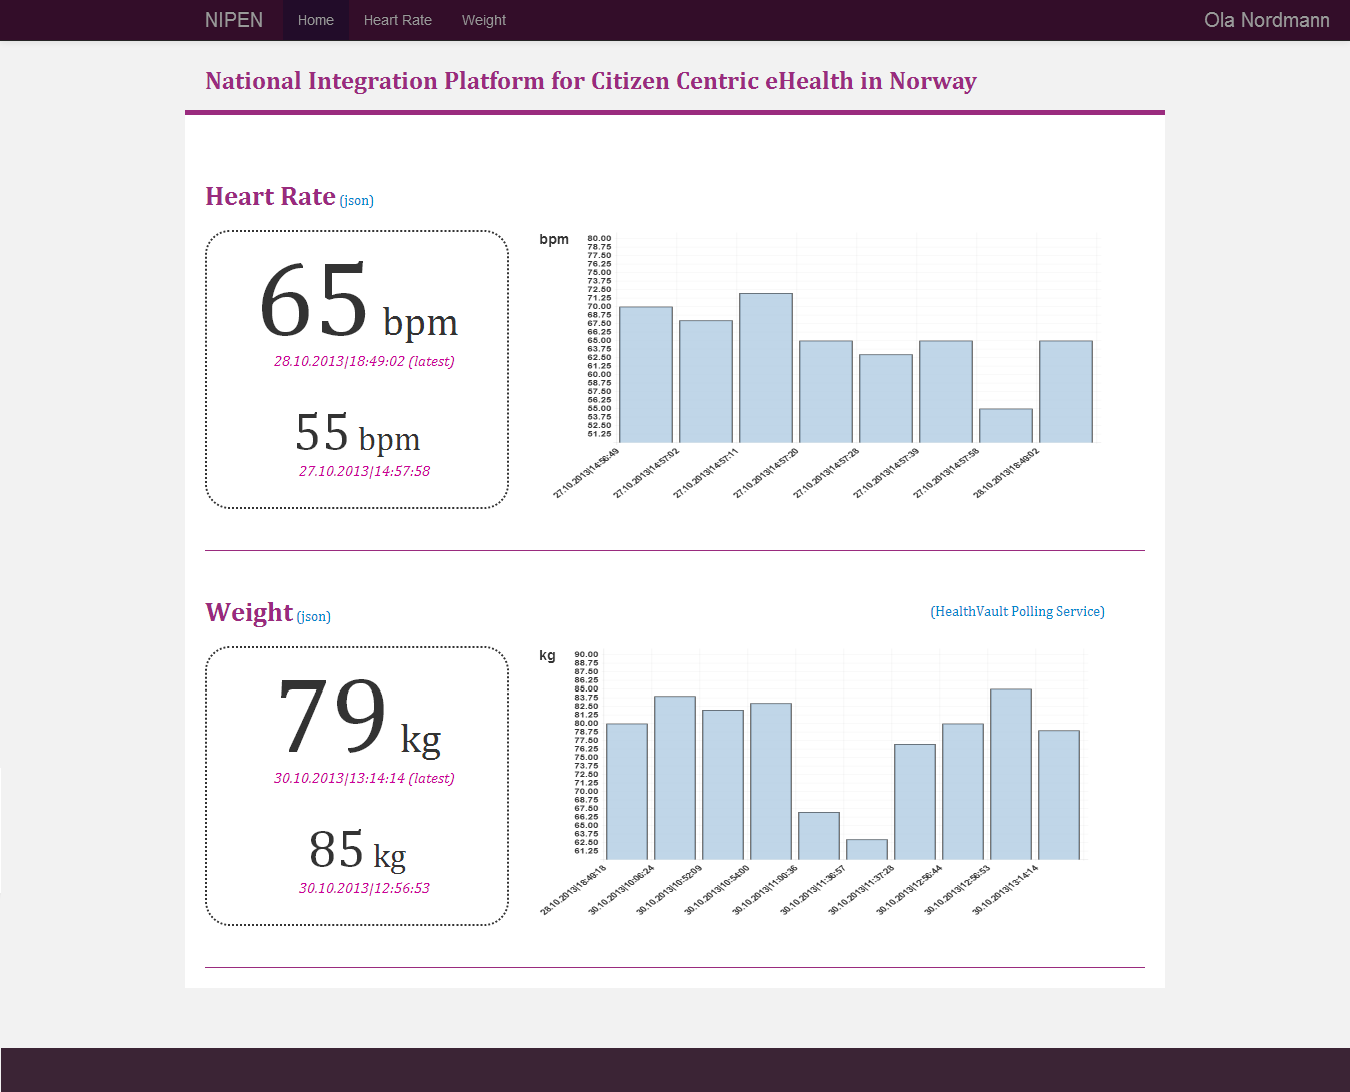
\includegraphics[scale=0.4]{../Figures/frontend-main-page.png}
\caption{Front-end home page}
\label{figure:frontend-main-page}
\end{figure}

\begin{figure}[H]
\centering
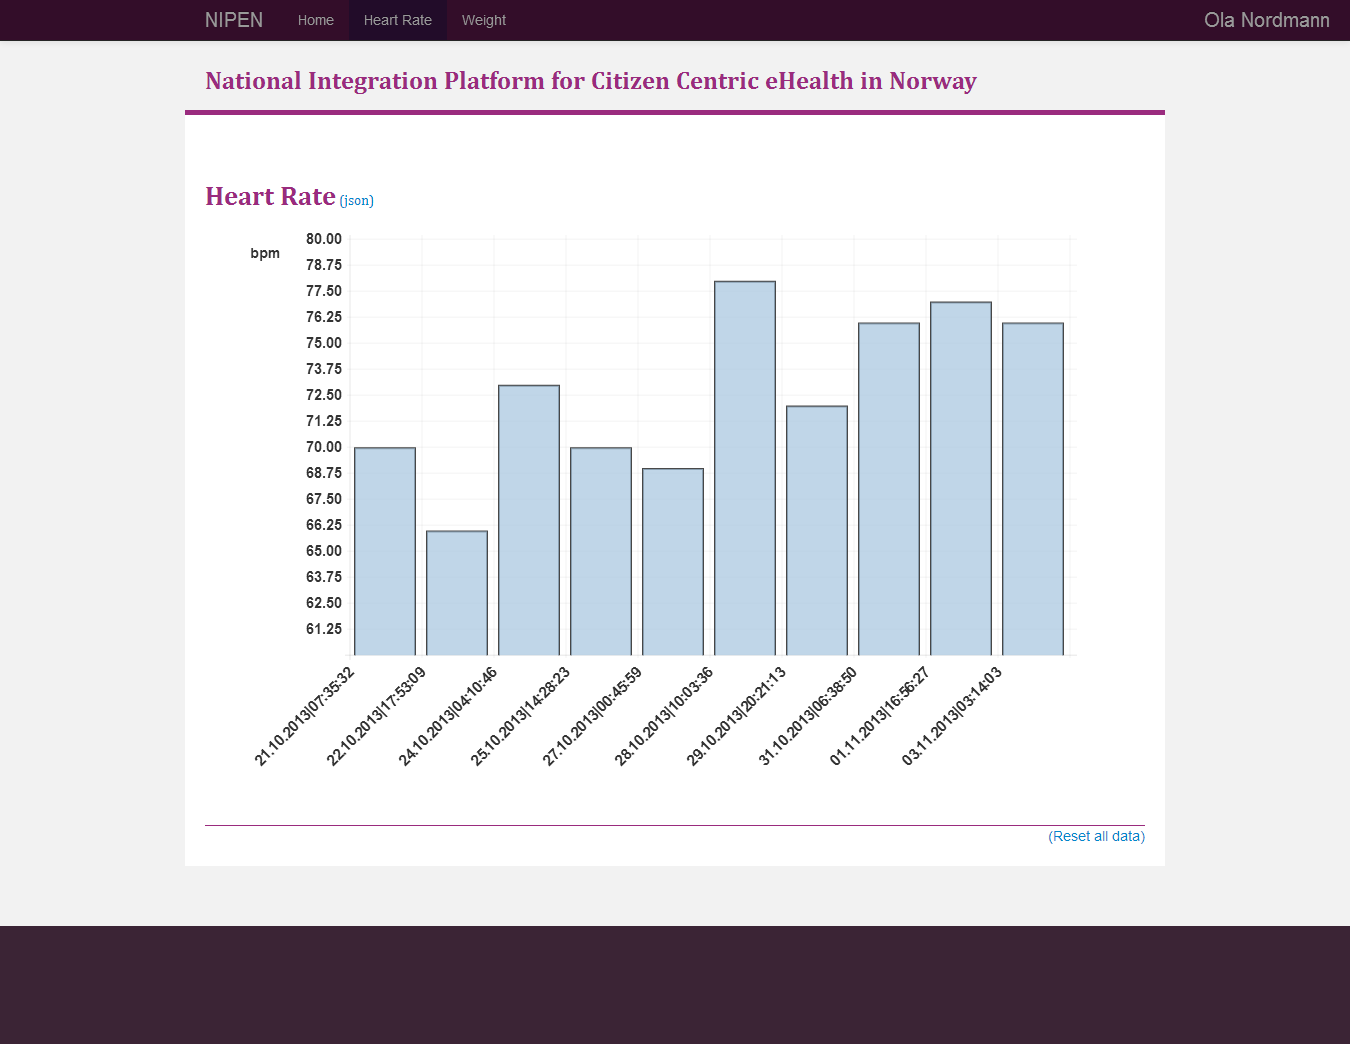
\includegraphics[scale=0.4]{../Figures/frontend-heart-rate-page.png}
\caption{Front-end heart rate page}
\label{figure:frontend-heart-rate-page}
\end{figure}

\begin{figure}[H]
\centering
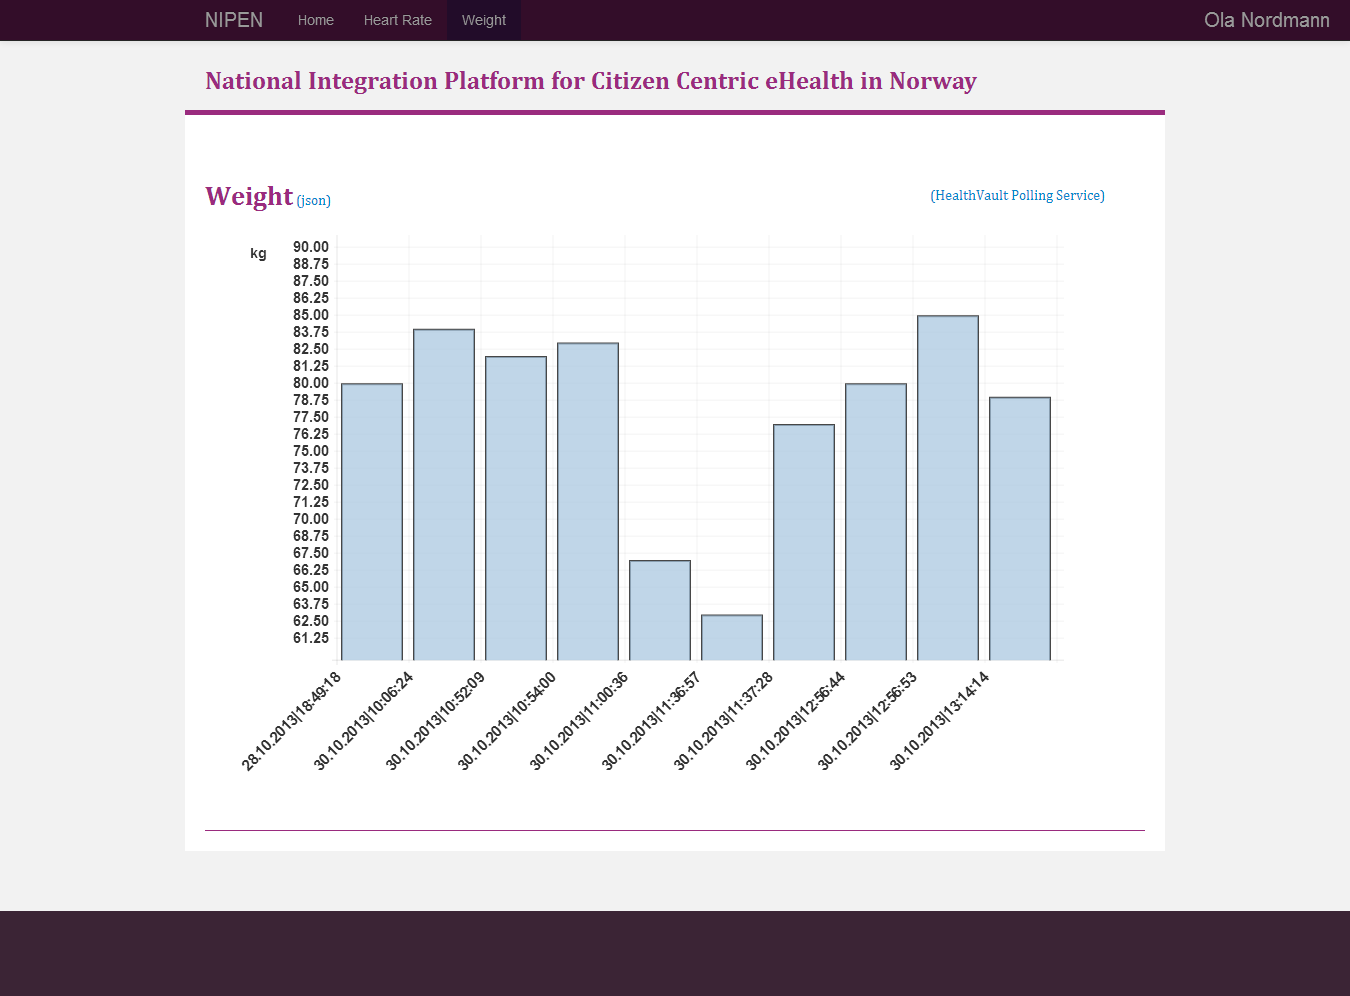
\includegraphics[scale=0.4]{../Figures/frontend-weight-page.png}
\caption{Front-end weight page}
\label{figure:frontend-weight-page}
\end{figure}

\subsection{Retrieving the Data}

To retrieve the data from NIPEN the front-end performs an API call just like any other application.
This is achieved by using AJAX through jQuery. An example \iffalse The structure of the call\fi is given below:
\begin{lstlisting}[language=JavaScript]
$.ajax({
  url: url, // the URL address, e.g.: <server address>/nipen/api/human/weights
  dataType: "json", // the data type of the received data, in this case a JSON string
  success: function(data) {
	// update web page here with the received data
  }
});
\end{lstlisting}

Accessing the JSON data with JavaScript is easy.
%Let's say that the data parameter, of the success function given above, consists of the following JSON array:
Let's say that the data parameter, of the success function given above, consists of the JSON array show precendently 
in subsection \ref{listing:jsonarray}.

\iffalse
\begin{lstlisting}[language=json]
[{
	"id":1,
	"userId":1,
	"timestamp":"2013-10-25 14:57:39.0",
	"value":80,
	"unit":"kg"
},
{
	"id":2,
	"userId":1,
	"timestamp":"2013-10-30 16:40:30.0",
	"value":81,
	"unit":"kg"
}]
\end{lstlisting}
\fi

Then the data can be accessed the following way:
\begin{lstlisting}[language=JavaScript]
data[0].id // returns 1
data[0].userId // returns 1
data[0].timestamp // returns "2013-10-25 14:57:39.0"
data[0].value // returns 80
data[0].unit // returns "kg"

data[1].id // returns 2
data[1].userId // returns 1
data[1].timestamp // returns "2013-10-30 16:40:30.0"
data[1].value // returns 81
data[1].unit // returns "kg"
\end{lstlisting}

This data is used in an update function, that updates all the values that are needed on the web page.
%% not really clear what you mean here.

\subsection{Polling}

We decided to implement polling on our front-end, since we are using AJAX to update the page.
AJAX is asynchronous which means that it can poll data in background without the need of refreshing the page.
Thus we don't need to update the web page when new data is received at NIPEN.
The jQuery AJAX function is polling constantly in the background when the client views the page.
When the front-end detects that new data is received, the JavaScript methods will update the page.
To detect if the data received from NIPEN is new, we compare the timestamp of the latest value on the web
page and the data received.
If this value is different, the charts and values on the web page needs to be updated.
This will be done automatically.
Of course, if data is added with a timestamp that contains a date earlier than the latest, then the web page 
will not be updated.
In this scenario the user must manually refresh the web page.

\section{Heart rate application}

The heart rate application is an application for Android mobile devices.
It's purpose is twofold: on one side it demonstrates the praticality of gathering health parameters using mobile phones,
on the other, it shows how easily these can be intregrated with NIPEN. % memorized, stored ?
The application was developed using an open source project called \verb|android-heart-rate-monitor| described
in subsection \ref{subsec:hr} which features an algorithm to measure heart rate using the phone's camera.
%We are using the open source  \cite{AndroidHeartRateMonitor} app as our base to our hart rate application.
Not having to implement such functionality ourselves allowed us to dedicate time to other tasks.
Being only three people on a large project like this, we though that it would be great idea.
%The existing android heart rate monitor app is capable of measuring a users heart rate.
We have extended the application to be able to send measurements to NIPEN.
To do so, the application constructs a valid JSON string representing an heart rate model and then
sends an HTTP POST message to the appropriate API endpoint containing the JSON string as payload.

%% this is mostly okay but too long to be this detailed.
%% i summarized it in a few senteces cutting out some boring details
\iffalse
To construct a valid heart rate JSON string we need user ID, timestamp, value and a unit. 
An ID is not needed because it is constructed at the back-end.
The user ID is a hard coded value, since we are only focusing on one user.
From the android device we are able to get the current time, the heart rate value is calculated through the
app and the unit is BPM (beats per minute).
With this information we are able to construct the JSON string that is needed to push a heart rate value into NIPEN.

To send the JSON string, we need to create an HTTP connection with NIPEN.
We are using the java class \textit{java.net.HttpURLConnection} for this task.
To initialize the URL connection we need to set the request method to POST and the content type to \textit{application/json}.
The URL is set to \textit{http://mhealthdemo03.cloudapp.net/nipen/api/human/heart\_rate}, where \textit{mhealthdemo03.cloudapp.net} is the server location as of this writing.
From the http connection we are able to get an output stream where we write the JSON message.
If we are not getting an exception at this stage, it means that the data was successfully transmitted.
\fi

A simple sequence diagram of how the application works is presented in figure \ref{figure:sending-heart-rate-through-app}.
What we have added to the application is the last part, i.e. from where the users presses the button.

\begin{figure}[h]
\centering
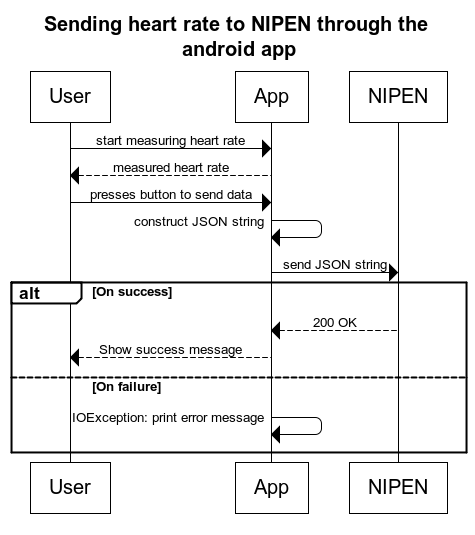
\includegraphics[scale=1.0]{../Figures/sending-heart-rate-through-app.png}
\caption{Sending a heart rate through the android app}
\label{figure:sending-heart-rate-through-app}
\end{figure}

\section{Weight application}

The weight application is an Android app that is able to fetch and push data to and from HealthVault, as well as
it is it capable of pushing data to NIPEN.
We are also using an existing solution as a base for this application, where the features we implemented are
the interactions with NIPEN.
The base we are using for this application is an example from the HealthVault Java SDK \cite{HealthVaultSDK}.
When the SDK is downloaded, it contains a folder named \textit{android}. 
This folder again contains a folder \textit{examples} where the base, we are using, is located.

When the application starts it asks the user to sign in to HealthVault.
If this is the first time the user uses this application he/she is asked to add this application to HealthVault,
after the sign in process.
When the user grants permission to the application, it is allowed to push and fetch data to and from HealthVault.

How the application works (after login) is illustrated in figure \ref{figure:sending-weight-to-healthvault-and-nipen}.
The functionality we implemented is the construction of the JSON string and the sending of the data to NIPEN.
This is developed almost exactly as the heart rate application, and hence is not further explained here.
The only difference is that we are creating a weight measurement instead of a heart rate.

\begin{figure}[h]
\centering
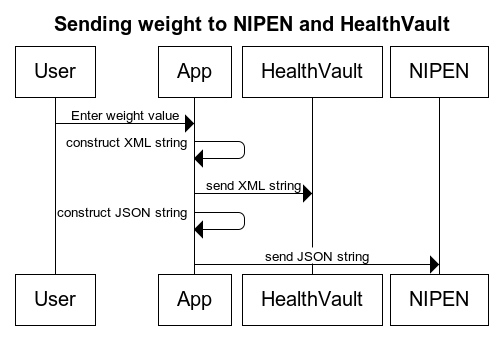
\includegraphics[scale=1.0]{../Figures/sending-weight-to-healthvault-and-nipen.png}
\caption{Sending weight to HealthVault and NIPEN}
\label{figure:sending-weight-to-healthvault-and-nipen}
\end{figure}

This application illustrates that it is possible to connect HealthVault into NIPEN.
If the user adds this application to HealthVault, it has access to all the weight values the user has added to the HealthVault account.
Thus it is possible to thereafter send the values into NIPEN.

\section{HealthVault Integration Service}

The HealthVault integration service is capable of retrieving values from HealthVault and send new values into NIPEN. 
As the weight application, this service uses an example in the HealthVault Java SDK \cite{HealthVaultSDK} as its base.
In the SDK folder it is located inside \textit{java-1.4.2} folder.
The functionality we have implemented into this application is a polling service and the interactions with NIPEN.
We have also made some cosmetic changes to the web pages the example provided.

This application consists of a back-end and a front-end.
What this means is that it consists of a web page and a server application.
The server application is handling the interactions with HealthVault and NIPEN, while the front-end creates a display for the user as well as it processes the users requests.

We have completely changes the look of the front-end of this application.
When the user opens the web page, he/she is asked to login into HealthVault.
The procedure for the login is the same as the weight application.
Figure \ref{figure:webservice-login} shows how the login page looks like.
After the user has signed in, a web page is shown where it is possible to start/stop the polling service.
Is is also possible tof push weight data into HealthVault. 
This is illustrated in figure \ref{figure:webservice-not-polling} and \ref{figure:webservice-polling}.

\begin{figure}[H]
\centering
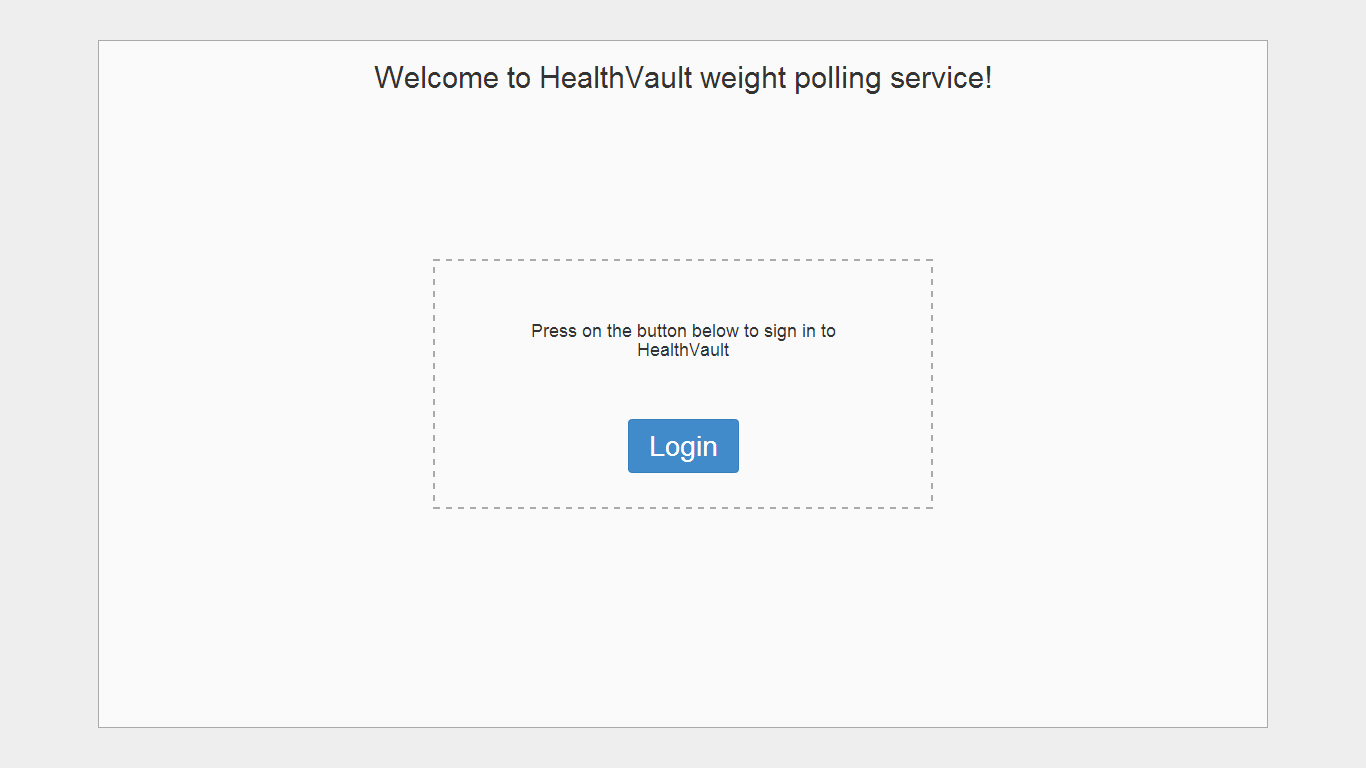
\includegraphics[scale=0.4]{../Figures/webservice-login.png}
\caption{HealthVault Integration Service login page}
\label{figure:webservice-login}
\end{figure}

\begin{figure}[H]
\centering
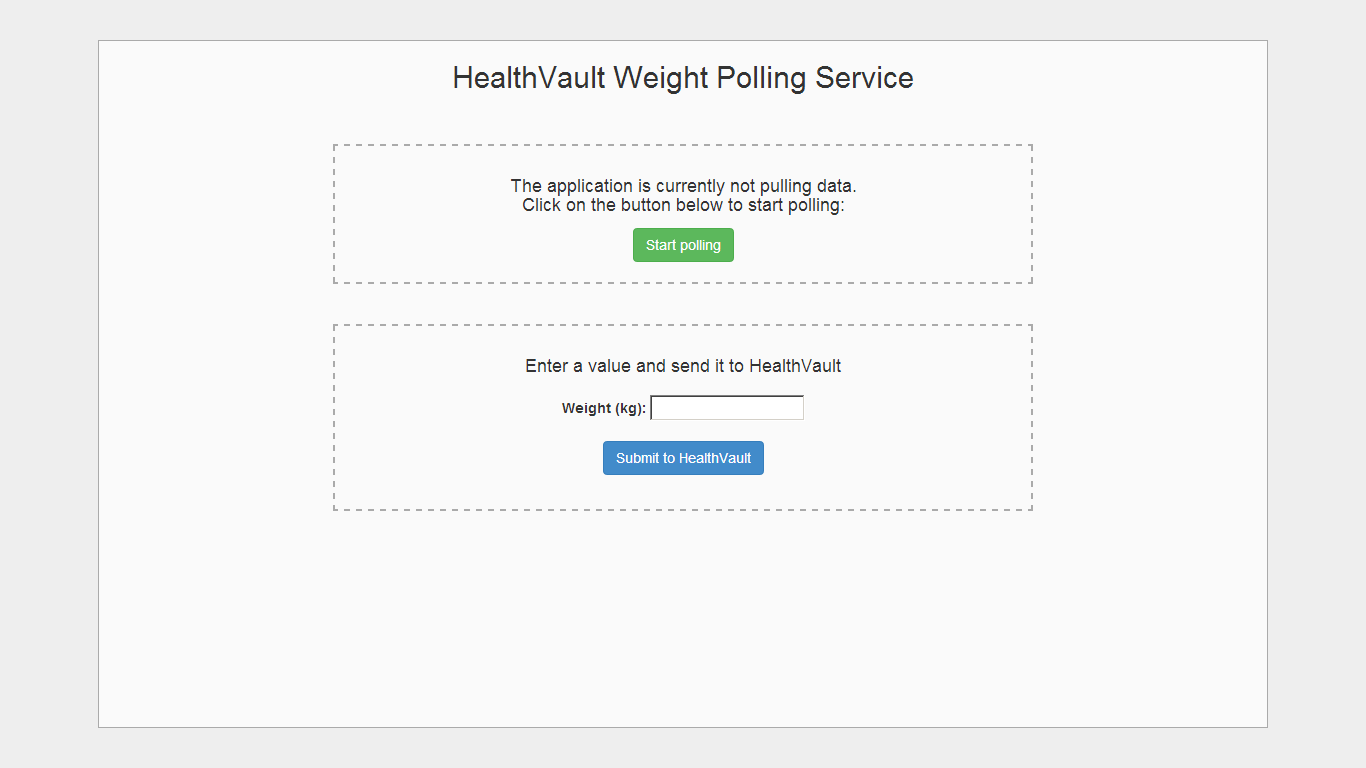
\includegraphics[scale=0.4]{../Figures/webservice-not-polling.png}
\caption{HealthVault Integration Service not polling page}
\label{figure:webservice-not-polling}
\end{figure}

\begin{figure}[H]
\centering
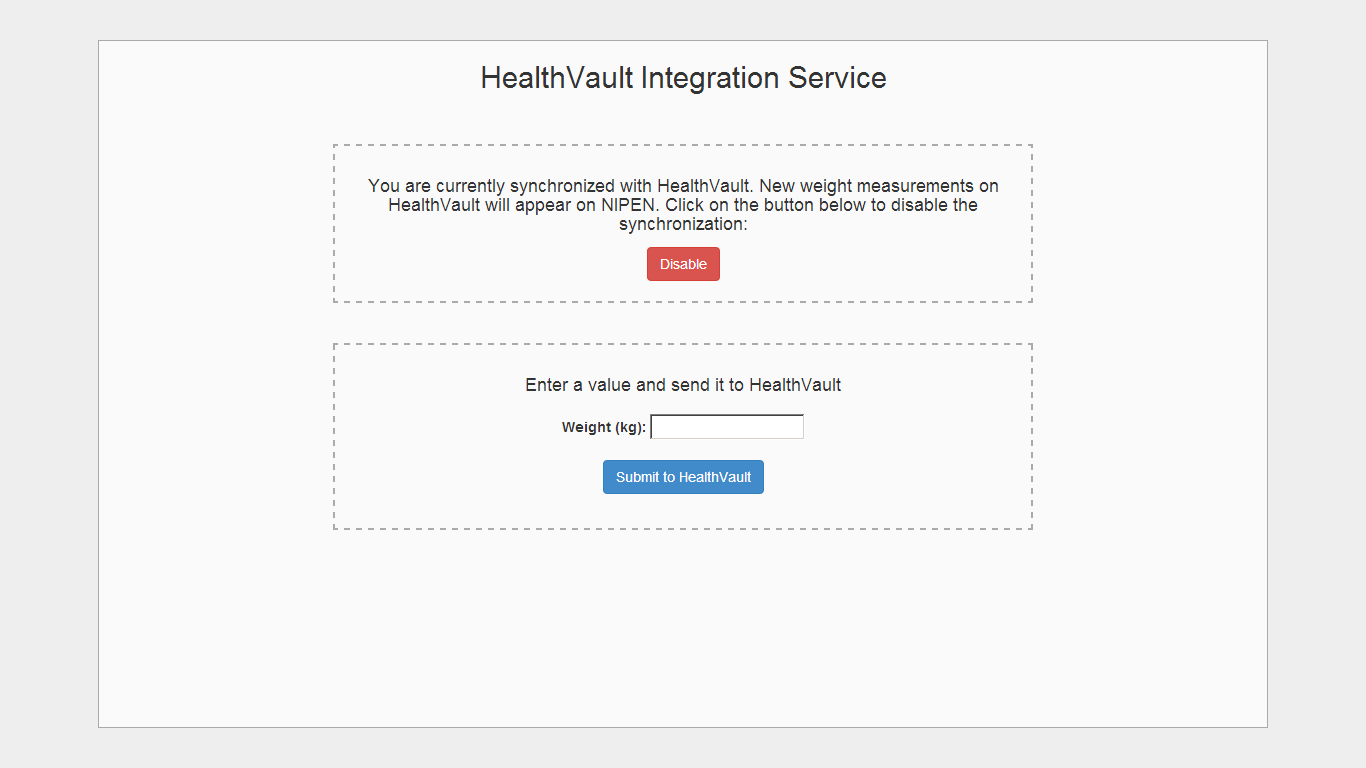
\includegraphics[scale=0.4]{../Figures/webservice-polling.png}
\caption{HealthVault Integration Service polling page}
\label{figure:webservice-polling}
\end{figure}

When the user has signed in to HealthVault through the application, an authentication token is sent from HealthVault.
This token is received and stored in the web service.
What this token does is that it allows the application to fetch weight data from HealthVault.
After the sign in the user can start the polling service.
When the user requests the application to start polling, a thread is created on the back-end.
This thread starts fetching data from HealthVault on a regular basis.
Every time the application receives data it waits 1 second and then fetches again.
This is repeated until the user stops the polling service.

When the polling starts the application stores the first timestamp, of the last weight measurement, received from HealthVault.
After that, for each poll the application compares this timestamp with the timestamp received from HealthVault.
A new value has been added to HealthVault if the timestamps are not equal.
If a new value has been detected, the application creates and sends a JSON string to NIPEN in the same way as the heart rate and weight application.
The polling service is illustrated in figure \ref{figure:weight-polling-service}.

\begin{figure}[h]
\centering
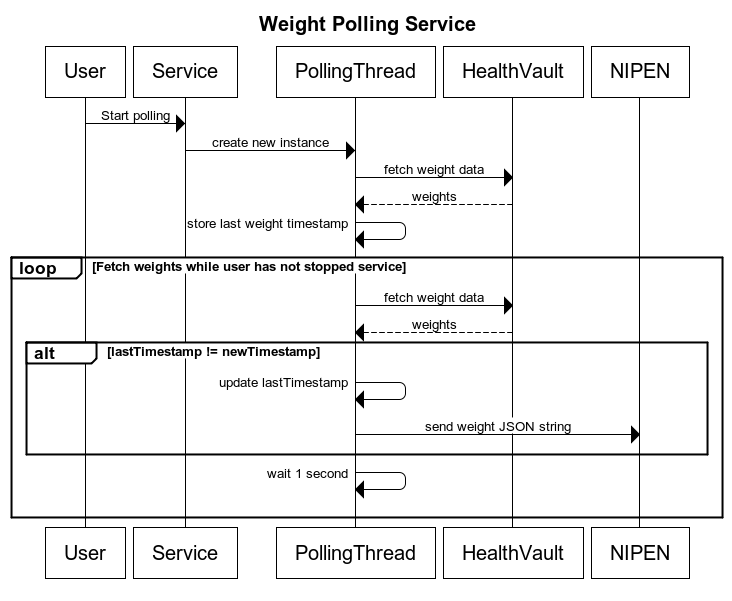
\includegraphics[scale=0.8]{../Figures/weight-polling-service.png}
\caption{HealthVault Integration Service sequence diagram}
\label{figure:weight-polling-service}
\end{figure}

\section{Conclusion} 
% Chapter Template

\chapter{Sprint 0} % Main chapter title

\label{Sprint 0} % Change X to a consecutive number; for referencing this chapter elsewhere, use \ref{ChapterX}

\lhead{Chapter 9. \emph{Sprint 0}} % Change X to a consecutive number; this is for the header on each page - perhaps a shortened title


\section{Planning}
what we planned to do
shall we include some data from scrumdo? definitely a chart..
\section{Duration}
\section{Goals}
what did we expect to achieve by the end of this sprint (general progress in the project)
\section{Feedback}
from customer, from supervisor
\section{Problems}

\section{Evaluation}
our thoughts about this sprint
 


\chapter{Sprint 1}
\label{Sprint0}
\lhead{Chapter 7. \emph{Sprint 1}}

\section{Goal(s)}

This sprint's goal was the completition of an initial prototype of the system whose functionality
had to be demonstrated to the customer; this corresponded to project milestone M1.
The purpose of such prototype was to act as a proof-of-concept and give the customer
a chance to express some feedback upon which we hoped to start a discussion
on possible improvements and new features.

Additional goals were the completion of project's planning and documents such as:
\begin{enumerate}[a)]
\item system requirements (both functional and non-functional)
\item report's table of contents
\item concrete work plan
\item risk analysis
\item test plan
\end{enumerate}

\section{Planning}

We planned to begin with an initial design and implementation of every part of the system which included:
\begin{enumerate}
\item the frontend, implementing the graphical user interface
\item the backend, implementing the logic of the API
\item the database, implementing persistency
\item the Android application to measure heart rate.
\end{enumerate}
During the first week development was to be done parallel to additional studies and documentation.
The second week we planned to work exclusively on development in view of the impending milestone.

\section{Duration}
The duration of the sprint was the following:
\begin{itemize}
\item Start: September, 9th
\item Milestone M1 (first system prototype): September, 20th
\item End: September, 22nd
\end{itemize}

\begin{figure}[H]
\centering
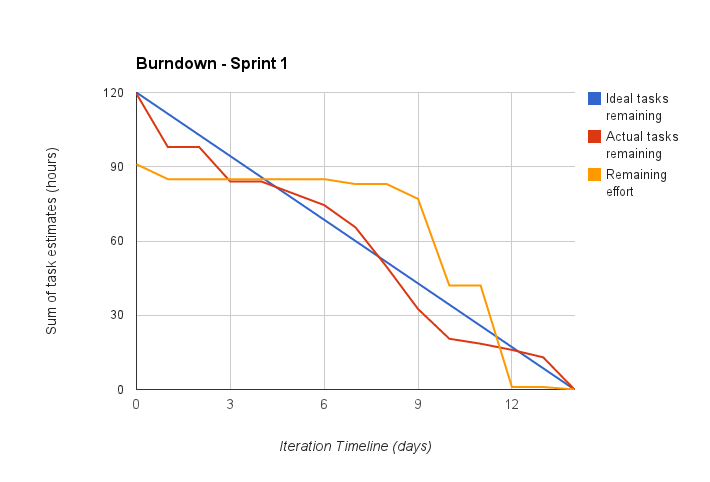
\includegraphics[scale=0.60]{../Figures/burndownSprint1.png}
\caption{Burndown chart Sprint 0}
\label{figure:burndownsprint0}
\end{figure}

\section{Backlog}

See below the sprint backlog.
\begin{itemize}
	\item \textbf{M1 First system prototype}
		Demonstrated to the customer on September, 20th.
		The demonstration was attended by the customer and two team members.
		The third team member participated remotely via Skype.
	\item \textbf{Project management}\newline
		This included:
		\begin{itemize}
			\item \textbf{Weekly startup meeting}: 
			\item \textbf{Meeting notes}:
				taking notes during meetings, reviewing of the notes.
			\item \textbf{Status reports}:
				for both week 37 and 38
			\item \textbf{Risk analysis}:
				updated on a weekly basis, so twice per sprint.
				The risk analisys was submitted to the supervisor and the customer.
			\item \textbf{Planning for the next iteration}:
				the project manager prepared a plan for the next iteration
				which would be illustrated and agreed upon on next iteration's startup meeting.
		\end{itemize}
	\item \textbf{Weekly meetings}
		includes meetings with both the customer and the supervisor.
		The meeting with the customer was held on Skype.
	\item \textbf{Additional pre-studies}
		Continued studies on relevant technlogies such as:
	\begin{itemize}
		\item \textbf{HealthVault}: Microsoft's online health platform.
		\item \textbf{Apache Camel}: a routing engine for enterprise integration patterns.
		\item \textbf{Javascript libraries for charts}: to be used in the frontend.
	\end{itemize}
	\item \textbf{System development}
		Initial design and implementation. This accounted for:
	\begin{itemize}
		\item \textbf{Backend development}:
			Development of Spring controllers for API endpoints. Database (DAO) coding to
			implement data persistence.
		\item \textbf{Frontend development}:
			Coding of the frontend. This included setting up an HTML page which used
			AJAX to perform API calls and JS to show the data retrieved using a bar chart.
		\item \textbf{Deployment}:
			Deployment of both backend and frontend using a servlet container (Tomcat).
	\end{itemize}
	\item \textbf{Heart rate application}:
		basic implementation of the Heart rate application. The application should be able to acquire
		the user's heart reate and send perform an API call to store the data on the backend.
	\item \textbf{Database development}:
		choose a suitable database to use for implementing persistency on the backend.
		Deploy the database and create a table for the heart rate.
	\item \textbf{Testing}:
		Perform unit and integration testing for the heart rate application and the backend.
\end{itemize}


%% i actually dont think having a table for this is a good idea. tables can't have much information
%% also it would require a lot of tweaking to get the estimated/actual times to look reasonable.
%% maybe a textual description would be better so we can omit some details in favor of others.
\iffalse
\begin{table}
\begin{tabular}{ | l | l | l | l | }
 \hline
  Story ID & Description & Size & Assignee \\
  \hline\noalign{\smallskip}\noalign{\smallskip}\hline
  33 & Project Management			& 8	& Emanuele  \\
  12 & M1 First System prototype	& 0 & All		\\
  45 & Weekly meetings (week 37)	& 6 & All		\\
  42 & Additional pre-studies		& 5 & Emanuele	\\
  \hline
\end{tabular}
\caption{}
\label{}
\end{table}
\fi

\section{Results and feedback}

Around the end of this sprint, on September 20th, we demonstrated a prototype of system to
the client which included: a) the frontend, b) the backend, c) an Android application to measure
heart rate using the phone's camera.

The backend supported web API calls for storing and retrieving heart rate measurements.
Both the Android application and the frontend used these API calls for sending and retrieving
such measurements respectively.
The measurements were ultimately shown to the user on a webpage (the frontend) using a bar chart.
We opted for MySQL as database to implement persistency on the backend due to the familiaritywe had with it.
We deployed it on the server machine and added a first table so that we could test the web API.
%functionality of the backend.
The customer was pleased with the results, stating that they were above his expectations.
We discussed about which features he would like to see implemented next in the product
and we agreed to prioritise interoperability with HealthVault instead of Withings.
The reason behind this decision was the fact that interoperability with HealthVault would have
enabled the product to use third-party devices supported by HealthVault to gather health data.
Since the number of devices supported by HealthVault is substantial, this was deemed a
desiderable feature for the product.
The customer asked if the amounts of resources we had at disposal to actually implement
such interoperability was sufficient and inquired about the general viability of such approach.
We expressed our confidence about its feasibility and that the resources at hand were sufficient.
Nevertheless, we set a deadline (10 days) to assess such feasibility in order not to delay
the general progress of the product.

Figure \ref{figure:demonstration-m1} shows the team demonstrating the product (who took the picture).
Emanuele is holding his mobile phone running the Heart rate application.
Sebastian is pointing at the frontend, displaying the data being acquired successufully.
Anders is participanting to the conversation through Skype.

\begin{figure}[h]
\centering
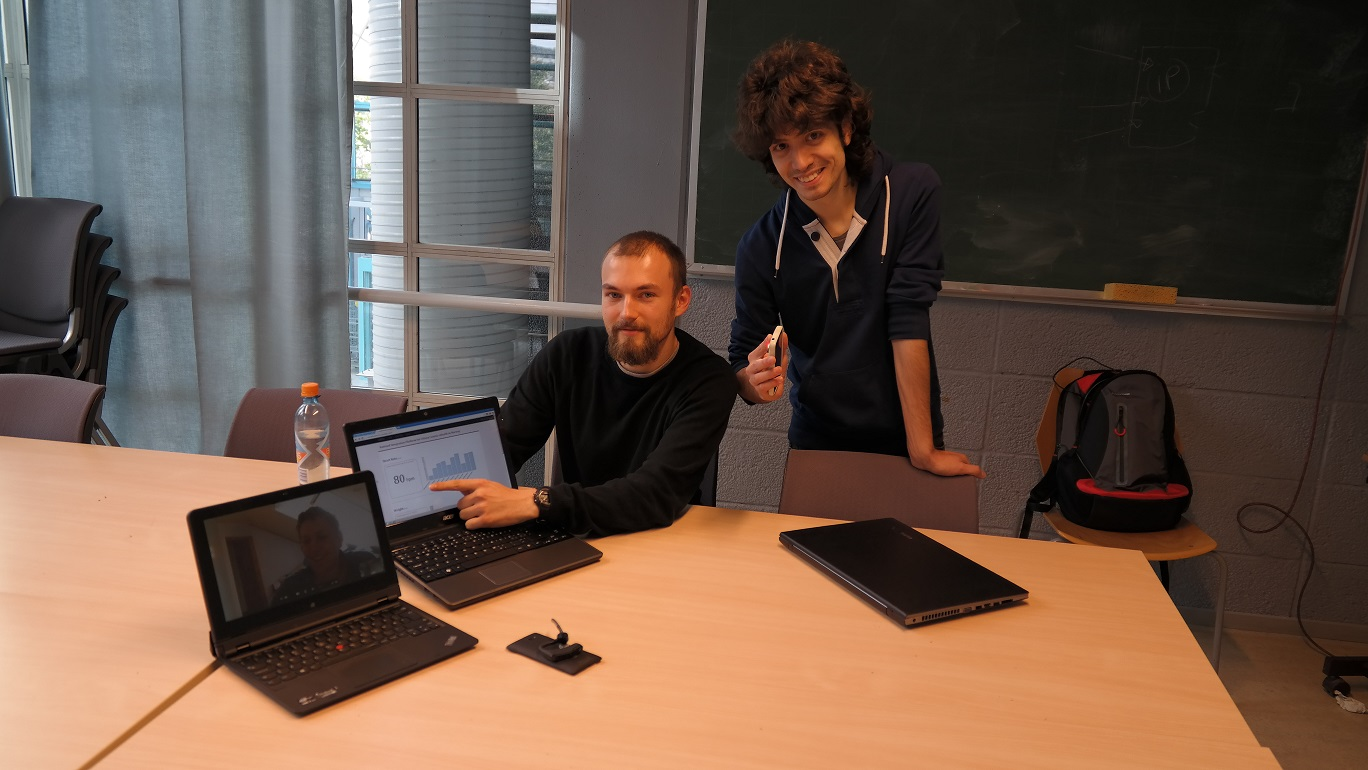
\includegraphics[scale=0.33]{../Figures/demo-m1.png}
\caption{Team demonstrating the product}
\label{figure:demonstration-m1}
\end{figure}

\textbf{Notes}: by the end of the sprint one team member had found a job and moved permanently to Oslo.
He expressed his continued committment to the project and told the other members that he would continue
to contribute to the project remotely.

\section{Evaluation}

The sprint was successful as we managed to achieve the main goal of the sprint (Milestone M1).
We were pleased by the positive feedback received from the customer and felt motivated to
keep up the good work. Furthermore, having proactively partecipated in the improvement/proposal
of product requirements together with the customer made the whole team look forward to implement these new
features and improve the product. Although we didn't manage write anything in the report we still had enough
time ahead to make up for it so we consider that a minor issue.
Development times for the Android application were dramatically reduced thanks to the functionality
offered by android-heart-rate-monitor (described in section \ref{ch:studies}).

%Due to timing issues we didn't manage to produce all the documentation we planned to.
%In particular we were missing the table of contents of the report and  

\chapter{Sprint 2}
\label{Sprint2}
\lhead{Chapter 8. \emph{Sprint 2}}

\section{Duration}
The duration of the sprint was the following:
\begin{itemize}
\item Start: September, 23rd
\item End: October, 6th
\end{itemize}

\section{Planning}

Having just demonstrated the product to the customer during the previous sprint, 
most of the work planned for this sprint was documentation writing in view of the second milestone.
This included writing the report itself but also reviewing other documents such as the
templates, notes and agendas.

During last sprint, we agreed with the customer to prioritise interoperability with
HealthVault rather than Withings.
For this purpose, we adjusted our plan accordingly and tasked one team member
to study HealthVault's SDK in order to determine the complexity of the task.

Additionally, we planned to continue with development and add support for weight
measurements to the API.

Although one member of the team would be working remotely from another city,
we thought it would be easy for him to collaborate in writing the documentation
so we did not prepare a separate work plan for him.
We did, though, schedule an internal meeting to be held weekly on Mondays
to keep in touch and share information about the project's progress.


\section{Goal(s)}

The main goal for this iteration was to write the report in view of the second milestone deadline
for mid-term delivery (M2). Additional goals were assessing the practicality of interoperability
with HealthVault and adding support for weight measurements to the API.



\section{Results and feedback}

We wrote a table of contents for the report and parts of the initial chapters as well.
The table of contents was submitted to the supervisor in order to make sure we weren't leaving out
any important chapter in our report. The team member who had moved to Oslo was able to contribute
to the project by writing the report.

Studies on HealtVault went smoothly. We were confident that we could fulfill the customer requirest
and came up with the idea of writing another Android application which would fetch some weight
measurements from HealthVault and send them to our integration platform.
We presented this idea to the customer after a few days and he agreed on it.
We then started some preliminary development on it which proceeded smoothly.
This was also thanks to HealthVault's SDK which greatly reduced the amount of code we needed
to write ourselves from scratch. We used one of the examples provided with the SDK which featured
out-of-the-box interoperability with HealthVault and added the functionality required to implement
interoperability with NIPEN.

System development also proceeded smoothly and we added support for the weight data to the backend.
The frontend and the database needed little work to accomodate these additions, so most of the work done on
them was minor tweakings.

\section{Evaluation}

\begin{figure}
\centering
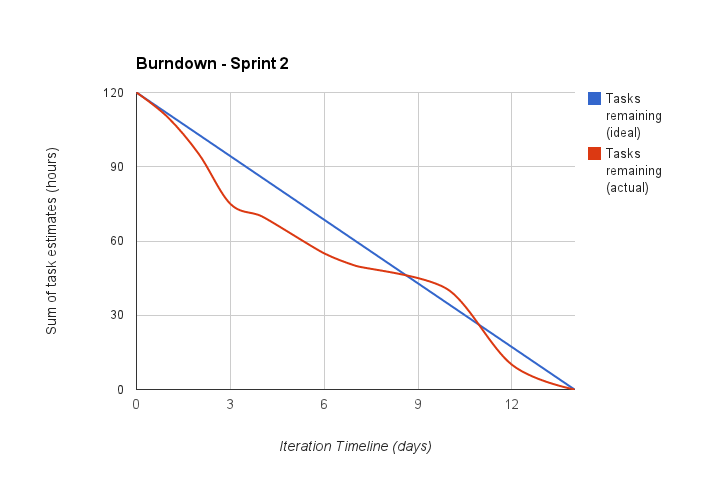
\includegraphics[scale=0.60]{../Figures/burndownSprint2.png}
\caption{Iteration burndown chart}
\label{figure:burndownsprint2}
\end{figure}

Results for this sprint were positive. We were pleased with how the report was shaping up and
received good feedback on our structure from the supervisor.

Our plan to let our colleague in Oslo work on the documentation worked out pretty well
and he was able to work indipendently and effeciently. Although he had moved to Oslo,
he didn't start to work right away so he a lot of time to dedicate to the project.

Since we had told the customer that we would be working primarily on the report for this sprint,
he didn't put any pressure on us to develop new features. We actually could not reach to him
the first week after the demonstration but this has not been an issue at all since we
knew what to work on. We were happy that our project was well in schedule with our plan so far.
This iteration burndown chart is shown in figure \ref{figure:burndownsprint2}.

\clearpage
\section{Backlog}

See below the sprint backlog.
\begin{enumerate}[1.]
	\item \textbf{Project management} included:
	\begin{itemize}
		\item \textbf{Sprint startup meeting}:
			included sprint planning and review
		\item \textbf{Weekly meetings}:
			with both the customer and the supervisor
			%*During week 39.we were unable to contact the customer. This was not a problem*
		\item \textbf{Meeting notes}:
			taking notes during meetings, reviewing of the notes
		\item \textbf{Status reports}:
			for both week 39 and 40
		\item \textbf{Review templates}:
			to be adopted for status reports and other documents
		\item \textbf{Risk analysis}:
			updated on a weekly basis
	\end{itemize}
	\item \textbf{Report work}\newline
		start writing the report, focus on necessary chapters for the mid-term delivery
	\item \textbf{HealthVault studies}\newline
		perform further studies in order to assess the feasibility of developing a prototype
		application that implemented interoperability with Microsoft's platform
	\item \textbf{System development}\newline
		preliminary development on the backend to accomodate the new weight API
	\item \textbf{Weigther application development}\newline
		initial design and implementation of a prototype application using the weight API.
		The application needs to connect to HealthVault and retrieve some weight measurements
		and then send them to the integration platform.
\end{enumerate} 


\chapter{Sprint 3}
\label{Sprint0}
\lhead{Chapter 9. \emph{Sprint 3}}

\section{Goal(s)}

The main goal of this sprint was the mid-term delivery of the report; this corresponded to
the second project's milestone M2. Furthermore, another important goal was finalizing the design and continuing
the development of the second prototype of the system which would feature HealthVault interoperability.

\section{Planning}

The plan consisted in an initial focus on report writing in order to receive as much
feedback as possibile on it. We understood that this was a good chance to receive
valuable feedback from a) the student advisor, b) the technical advisor, c) the customer.
We planned some additional system and application development after mid-term delivery
%At this point, we had a clear idea of what our second prototype would have consisted of.
%Also, we didn't want to fall behind schedule with system development so we planned some
%development as well

\section{Duration}
\begin{itemize}
\item Sprint start:  October, 7th
\item Milestone M2 (mid-term report delivery): October, 14th.
\item Sprint end: October, 20th
\end{itemize}

\section{Backlog}
See below the sprint backlog.

\begin{itemize}
\item \textbf{M2 Mid-term report}:
	delivery of the mid-term report. Although this delivery was not graded we made an effort
	to produce as much documentation as possible in order to receive extensive feedback from
	1) the student advisor 2) the technical advisor 3) the customer.
\item \textbf{Project management}\newline
	This included:
	\begin{itemize}
		\item \textbf{Weekly startup meeting}:
		\item \textbf{Meeting notes}:
			taking notes during meetings, reviewing of the notes.
		\item \textbf{Status reports}:
			for both week 41 and 42
		\item \textbf{Risk analysis}:
			updated on a weekly basis, so twice per sprint.
			%% The risk analisys was submitted to the supervisor and the customer.
		\item \textbf{Planning for the next iteration}:
			the project manager prepared a plan for the next iteration
			which would be illustrated and agreed upon on next iteration's startup meeting.
	\end{itemize}
	\item \textbf{Weekly meetings}: 
		meetings with both the customer and the supervisor. Beginning this sprint, the first
		planned after one team member moved to Oslo, we scheduled an internal meeting with him
		to be held once per week.
	\item \textbf{Application development}:
		continued development of the Android application.
	\item \textbf{System development}:
		we performed some studies on the different ways we could deploy the backend
		1) as a WAR file in a separate servlet container (Apache Tomcat) 2) as a Spring JAR file
		with embedded servlet support. Furthermore we continued development
	\item \textbf{Report work}:
		to be done by the team member in Trondheim.
	\item \textbf{Additional report work}:
		to be done by the team member in Oslo.
	\item \textbf{Testing}:
		produce some tests using an automated test suite.
\end{itemize}

\section{Results and feedback}

This sprint proceeded smoothly. We were able to write most of what we planned to and had no problems meeting
the deadline for the report mid-term delivery.
We were also generally satisfied with the quality of what had been written as we spent some time
reviewing the document as well.
We attended the lecture about technical writing at the end of which we received some positive feedback on the report.
Development proceeded without major issues. We were able to re-use good portions of code provided
by HealthVault's SDK, dramatically reducing the time spent on development. This let us spend more
time on other tasks.

We performed some major refactoring of the code on a dedicated Git branch in an effort
to a achieve a more 'neat' deployment solution which didn't require a separate servlet container like
Apache Tomcat but was entirely based on Spring using an embedded servlet-container.


Because one team member owned a Withings scale device, we thought it would have been
a good idea to include that in the demonstration of the second system prototype.

Since Withings supported integration with HealthVault natively, our plan to include
the scale in the demonstration was to use the scale to acquire a measurement, which would
then be sent over to HealthVault where our Android application would retrieve it and
send it over to NIPEN.

\begin{figure}[H]
\centering
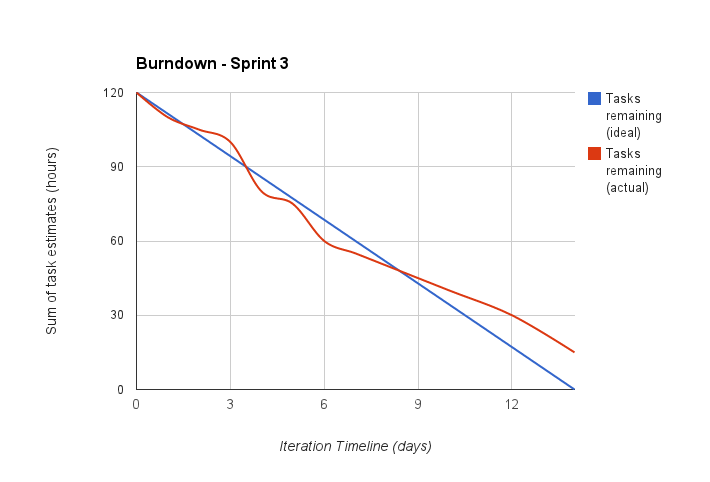
\includegraphics[scale=0.60]{../Figures/burndownSprint3.png}
\caption{Burndown chart Sprint 3}
\label{figure:burndownsprint3}
\end{figure}

\section{Evaluation}

All in all this sprint was successful.
However, refactoring was an unexpectedly time-consuming task.
Luckly, since all refactoring had been performed on a separte branch on Git, it didn't hinder
or delay any other activity as we always had a working branch for development and demonstration purposes.


 

\chapter{Sprint 4}
\label{Sprint4}
\lhead{Chapter 10. \emph{Sprint 4}}

\section{Duration}
The duration of the sprint was the following:
\begin{itemize}
\item Start: October, 21st
\item End: November, 03rd
\end{itemize}

\section{Planning}

This sprint's plan consisted in one last development effort to complete the second prototype
before our meeting with the customer and in view of the feature freeze deadline.

Although some refactoring done last sprint did result in a slight improvement to the codebase,
most of it did not make it make into the master branch because we did not have enough spare resources
to dedicate to this task, or we would have rather used those for report writing which
was becoming an increasingly pressing task.

Regarding the collaboration with our colleague in Oslo, we discussed his contribution
to the project during last sprint in an internal meeting.
We understood that it would have helped to be specific about what parts
of the report we expected him to write. We also made a more realistic estimate
of the amount of time he could dedicate the project being a full-time worker.
After these considerations, we planned less work for him for this sprint.
We were explicit about what parts of the report he should have worked on and
encouraged him to track his time appropriately.
We tried to make him feel part of the team and we counted on him.

\iffalse
For our colleague in Oslo, we planned documentation exclusively in order
not to fall behind with the status of the report.

Talking with him during an internal meeting, we understood that it would have helped to be specific
about what parts of the report we expected him to write.
Being cautious about the matter,
we planned less work for him for the next sprint but we were more explicit about what parts
of the report he should have worked on and encouraged him to track his time appropriately.
We tried to make him feel part of the team and we counted on him.
\fi

\section{Goal(s)}

The main goal of this sprint was to finalize and demonstrate a second prototype of the product,
which included: a) the backend, b) the frontend, c) two Android applications.
These had to be ready for October the 24th when our customer planned to visit Trondheim.

\section{Backlog}
See below the sprint backlog:
\begin{enumerate}[1.]
\item \textbf{Project management} included:
	\begin{itemize}
		\item \textbf{Sprint startup meeting}:
			included sprint planning and review
		\item \textbf{Weekly meetings}: 
			meetings with both the customer and the supervisor. Internal meeting with our colleague in Oslo
		\item \textbf{Meeting notes}:
			taking notes during meetings, reviewing of the notes
		\item \textbf{Status reports}:
			for both week 43 and 44
		\item \textbf{Risk analysis}:
			updated on a weekly basis
	\end{itemize}
	\item \textbf{System development}
		additional system development to accomodate fixes to the front end
	\item \textbf{Web application development}
		develop a web application which integrates weight measurements
		on HealthVault in our system
	\item \textbf{Report work}
		to be done by the team member in Trondheim
	\item \textbf{Additional report work}
		to be done by the team member in Oslo
	\item \textbf{Testing}
		perform unit and integration testing
\end{enumerate}

\section{Results and feedback}

During this sprint we worked mostly on development, which proceeded smoothly
with one exception. Withings integration with HealthVault, which we planned to use for
our demonstration, was not working as expected: Withings failed to send the data acquired
by the scale device to HealthVault. Unfortunately, after various attempts, we were unable to
solve the problem because we had no control over it.

A second prototype of the product was completed on schedule before our
planned meeting with the customer, which would have been on the 24th.
However, the customer canceled the meeting and proposed to reschedule it for the 30th.

Considering we had some more time to dedicate to development activities and in view
of the feature freeze deadline (M3) by the end of the sprint, we took initiative
and submitted a new possible application prototype idea to the customer.
It consisted of a web application which would feature HealthVault integration
similarly to the Android application.
The customer expressed his interest in it because it would have used a different
technology other than Android. He inquired about its feasibility in such a short amount
of time (less than two weeks). We were confident that we could have re-used some code
shipped with HealthVault SDK to minimize the amount of code we would have had to write
ourselves, so we committed its development.

On the 30th of November, very early in the morning the customer sent us a mail
were he canceled our meeting. However, he was available for a Skype meeting.
We were able to demonstrate him our product via Skype, including the last application
which had been developed in one week time. He was very pleased with our work.

\section{Evaluation}

The sprint was very rewarding.
Receiving a good evaluation from the customer proved to be very valuable for the group,
especially because the project was drawing to an end and timing was becoming tight;
there was no time left to make any big adjustments to the product.
The feedback from the customer motivated the group to keep up the good work
and make one big final effort to finish the documentation and prepare a presentation.
We discussed with the customer about the latter, and agreed to have an additional
presentation with the customer's colleagues after the 21st of November.

Although the scenario for the demonstration had changed and did not include
the Withings scale device anymore, the functionality of the application itself
had not, so we consider that a very minor issue.

Regarding our collaboration with our colleague in Oslo, he appreciated
our understanding of his situation and our attempts to plan a more
appropriate amount of work for him. He managed to contribute
more effectively during this sprint

 


\chapter{Sprint 5}
\label{Sprint0}
\lhead{Chapter 11. \emph{Sprint 5}}

\section{Duration}
The duration of the sprint was the following:
\begin{itemize}
\item Sprint start:  November, 4th
\item Milestone M3 (feature freeze): November, 4th.
\item Sprint end: November, 20th
\end{itemize}

This sprint was a bit longer than the others because it included the last days
that were left till the end project.

\section{Planning}

The plan for this sprint consisted primarily in report writing and review.
At the beginning of the sprint we arranged with the supervisor to deliver him a mostly finished version of the report by the end of the first week (around Sunday, the 10th) in order to let him give us some last feedback on it.

Regarding the inclusion of Withings in the demonstration scenario, we ultimately dropped it because we had no further time to look into it and we had come to a conclusion that it was not possible for us to fix it.
Furthermore, as already discussed, it would not have hindered the functionality of the product itself.

Since our product was completed on schedule, we were only left some integration and system testing.

\section{Goal(s)}

This was the final sprint of our project. 
Its main goal was to finalize the product and the documentation as well as prepare a presentation.

\section{Results and feedback}

Results for this sprint were largely positive. 
Although there wasn't much time left to complete the report and prepare the presentation, we managed to write quite a lot. 
We sent our supervisor a mostly finished version of our report on the 10th of November. 
He acknowledged our hard work and provided some positive feedback which contributed to further improvements in the quality of the report and motivated the group to keep up the good work. 
He offered to provide more feedback on an updated version of the report, which we submitted on the 17th.

\section{Evaluation}

\begin{figure}
\centering
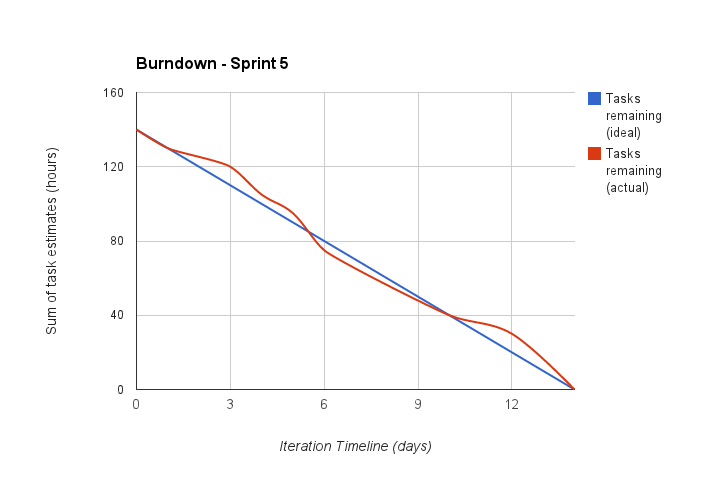
\includegraphics[scale=0.60]{../Figures/burndownSprint5.png}
\caption{Iteration burndown chart}
\label{figure:burndownsprint5}
\end{figure}

The sprint went smoothly. 
The feedback provided by the supervisor was very helpful and helped us to focus our efforts on those parts of the report that were lacking.
Unfortunately some team members were busy with other responsibilities, so the amount of time they could dedicate to the project was somewhat limited.
However, we were still pleased with the quality of the report.

This iteration burndown chart is shown in figure \ref{figure:burndownsprint5}.


\section{Backlog}
See below the sprint backlog.
\begin{enumerate}[1.]
\item \textbf{Project management} included:
	\begin{itemize}
		\item \textbf{Sprint startup meeting}:
			included sprint planning and review
		\item \textbf{Weekly meetings}: 
			meetings with both the customer and the supervisor. Internal meeting with our colleague in Oslo
		\item \textbf{Meeting notes}:
			taking notes during meetings, reviewing of the notes
		\item \textbf{Risk analysis}:
			updated on a weekly basis, so twice per sprint
	\end{itemize}
	\item \textbf{Report work}
		to be done by the team member in Trondheim
	\item \textbf{Additional report work}
		to be done by the team member in Oslo
	\item \textbf{Testing}
		perform integration and system testing
	\item \textbf{Presentation}
		prepare a presentation for the project
\end{enumerate}
 

\chapter{Testing}

\label{Testing}

\lhead{Chapter 12. \emph{Testing}}

\section{Testing methods}

\section{Tools}

\section{Functional tests}

\begin{table}
\begin{center}
\begin{tabular}{ | l | p{10cm} | }
	\hline
	\textbf{Test}	&	\textbf{ID 1} \\
	\hline\noalign{\smallskip}\noalign{\smallskip}\hline
	Name				& Heart rate REST (read) \\
	Requirement			& \hyperref[table:reqip]{FIP1} \\
	Description			& Test the REST endpoint for receiving heart rate data models \\
	Preconditions		& 	\par The IP is deployed and running on a server machine 
							\par The test is run on the server machine or alternatively
							one that has access to the server and whose address is replaced to the
							string \verb|localhost| in the test.
							\par The machine on which the test is run has the \verb|curl| program installed. \\
	Steps 				&	1. Run the following:
							\begin{verbatim}
							curl localhost:8080/nipen/human/api/heart_rates
							\end{verbatim}
							\\
	Postconditions		& A JSON valid, comma separated list of heart rate data models consistent with 
							entries in the databased hosted on the server. \\
	Results				& - \\
	Comments			& - \\
	Status				& OK or FAIL \\
	Tester				& Person \\
	Date				& dd-mm-2013 \\
	\hline
\end{tabular}
\end{center}
\end{table}

\begin{table}
\begin{center}
\begin{tabular}{ | l | p{10cm} | }
	\hline
	\textbf{Test}	&	\textbf{ID 2} \\
	\hline\noalign{\smallskip}\noalign{\smallskip}\hline
	Name				& Weight REST (read) \\
	Requirement			& \hyperref[table:reqip]{FIP2} \\
	Description			& Test the REST endpoint for receiving weight data models \\
	Preconditions		&	\par The IP is deployed and running on a server machine
							\par The test is run on the server machine or alternatively
							one that has access to the server and whose address is replaced to the
							string \verb|localhost| in the test.
							\par The machine on which the test is run has the \verb|curl| program installed. \\
	Steps 				&	1. Run the following:
							\begin{verbatim}
							curl localhost:8080/nipen/human/api/weights
							\end{verbatim}
							\\
	Postconditions		& A JSON valid, comma separated list of heart rate data models consistent with 
							entries in the database hosted on the server. \\
	Results				& - \\
	Comments			& - \\
	Status				& OK or FAIL \\
	Tester				& Person \\
	Date				& dd-mm-2013 \\
	\hline
\end{tabular}
\end{center}
\end{table}

\begin{table}
\begin{center}
\begin{tabular}{ | l | p{10cm} | }
	\hline
	\textbf{Test}	&	\textbf{ID 3} \\
	\hline\noalign{\smallskip}\noalign{\smallskip}\hline
	Name				& Heart rate REST (write) \\
	Requirement			& \hyperref[table:reqip]{FIP3} \\
	Description			& Test the REST endpoint for requesting heart rate data models \\
	Preconditions		&	\par The IP is deployed and running on a server machine
							\par The test is run on the server machine or alternatively
							one that has access to the server and whose address is replaced to the
							string \verb|localhost| in the test.
							\par The machine on which the test is run has the \verb|curl| program installed.
							\par At least one heart rate measurement has been stored on the IP \\
	Steps 				&	1. Run the following \begin{verbatim}
							curl -X POST -H "Content-Type: application/json"
							-d {"id":0,"value":60,"timestamp":"11-10-2013","unit":
							"bpm"}' localhost:8080/nipen/human/api/heart_rates
							\end{verbatim} \\
	Postconditions		& A database entry coherent with the JSON data submitted is created on the server. \\
	Results				& -- \\
	Comments			& - \\
	Status				& OK or FAIL \\
	Tester				& Person \\
	Date				& dd-mm-2013 \\
	\hline
\end{tabular}
\end{center}
\end{table}


\begin{table}
\begin{center}
\begin{tabular}{ | l | p{10cm} | }
	\hline
	\textbf{Test}	&	\textbf{ID 4} \\
	\hline\noalign{\smallskip}\noalign{\smallskip}\hline
	Name				& Weight REST (write) \\
	Requirement			& \hyperref[table:reqip]{FIP4} \\
	Description			& Test the REST endpoint for requeting weight data models \\
	Preconditions		&	\par The IP is deployed and running on a server machine
							\par The test is run on the server machine or alternatively
							one that has access to the server and whose address is replaced to the
							string \verb|localhost| in the test.
							\par The machine on which the test is run has the \verb|curl| program installed.
							\par At least one weight measurement has been stored on the IP \\
	Steps 				&	1. Run the following \begin{verbatim}
							curl -X POST -H "Content-Type: application/json"
							-d {"id":0,"value":60,"timestamp":"11-10-2013","unit":
							"kg"}' localhost:8080/nipen/human/api/weight
							\end{verbatim} \\
	Postconditions		& A database entry coherent with the JSON data submitted is created on the server. \\
	Results				& -- \\
	Comments			& - \\
	Status				& OK or FAIL \\
	Tester				& Person \\
	Date				& dd-mm-2013 \\
	\hline
\end{tabular}
\end{center}
\end{table}


\begin{table}
\begin{center}
\begin{tabular}{ | l | p{10cm} | }
	\hline
	\textbf{Test}	&	\textbf{ID 5} \\
	\hline\noalign{\smallskip}\noalign{\smallskip}\hline
	Name				& Heart rate measurement \\
	Requirement			& \hyperref[table:reqheartrate]{FHR1} \\
	Description			& Test the heart rate measurement functionality \\
	Preconditions		& The application has started \\
	Steps 				&	\par 1. User holds his finger on the camera applying a slight pressure \\
	Postconditions		&	\par 1. The icon on the left side of the screen is blinking 
							\par 2. A measurement appears after 4 seconds at most \\
	Results				& -- \\
	Comments			&	The measurement is expected to be rough.
							Any value between 60 and 100 is okay as long as it actually varies slightly based
							on the tester's perceived heart rate.  \\
	Status				& OK or FAIL \\
	Tester				& Person \\
	Date				& dd-mm-2013 \\
	\hline
\end{tabular}
\end{center}
\end{table}


\begin{table}
\begin{center}
\begin{tabular}{ | l | p{10cm} | }
	\hline
	\textbf{Test}	&	\textbf{ID 6} \\
	\hline\noalign{\smallskip}\noalign{\smallskip}\hline
	Name				& Login \\
	Requirement			& FR1 \\
	Description			& Test the login functionality \\
	Preconditions		& The application has started \\
	Steps 				&	\par 1. 
							\par 2. 
							\par 3. \\
	Postconditions		& The login screen disappear and the inbox appear \\
	Results				& -- \\
	Comments			& -- \\
	Status				& OK or FAIL \\
	Tester				& Person \\
	Date				& dd-mm-2013 \\
	\hline
\end{tabular}
\end{center}
\end{table}


\begin{table}
\begin{center}
\begin{tabular}{ | l | p{10cm} | }
	\hline
	\textbf{Test}	&	\textbf{ID 7} \\
	\hline\noalign{\smallskip}\noalign{\smallskip}\hline
	Name				& Heart rate measurement \\
	Requirement			& \hyperref[table:reqheartrate]{FHR3} \\
	Description			& Test the heart rate application interoperability \\
	Preconditions		&	\par 1. The application has started
							\par 2. A heart rate measurement has been acquired \\
	Steps 				&	\par 1. User presses \textbf{Send} button \\
	Postconditions		&	\par 1. The application shows a toast
							\par 2. The measurement is acquired by the Integration Platform \\
	Results				& -- \\
	Comments			& -- \\
	Status				& OK or FAIL \\
	Tester				& Person \\
	Date				& dd-mm-2013 \\
	\hline
\end{tabular}
\end{center}
\end{table}

\begin{table}
\begin{center}
\begin{tabular}{ | l | p{10cm} | }
	\hline
	\textbf{Test}	&	\textbf{ID 8} \\
	\hline\noalign{\smallskip}\noalign{\smallskip}\hline
	Name				& HealthVault data fetching \\
	Requirement			& \hyperref[table:reqweight]{FHV1} \\
	Description			& Test HealthVault connectivity \\
	Preconditions		&	\par 1. The application has started
							\par 2. The user has authenticated to HealthVault \\
	Steps 				&	\par 1. User \\
	Postconditions		&	\par 1. 
							\par 2. \\
	Results				& -- \\
	Comments			& -- \\
	Status				& OK or FAIL\\
	Tester				& Person \\
	Date				& dd-mm-2013 \\
	\hline
\end{tabular}
\end{center}
\end{table} 
\chapter{Conclusion}
\label{ch:conclusion}

This chapter covers the final state of the NIPEN project.
It at also discusses the state of all the requirements of the project.
At the end it talks about what the customer should do about future work on this project.

\lhead{Chapter 16. \emph{Conclusion}} 

\section{Fulfillment of requirements}

This section discusses how our project fulfills the requirements of the project. 
It explains the state of all the requirements and if they were completed. Each requirement had a priority which halped us identify what was important for us to focus on.

\subsection{Fulfillment of functional requirements}

This subsection describes the functional requirements for the product and their state after the project completion.
Our initial requirements were that this platform should both recive and deliver health data. 
The requirements were revised during the project with feedback from the customer.
The customer felt it was sufficent that the integration platform was able to receive health data and that it was more important to have a good sync with Microsoft HealtVault. 
The final product can out receive and deliver health data but there is no authentication on the delivering part in this prototype. 

\textbf{Fulfillment of functional requirements for the integration platform}

\begin{table}[H]
\begin{center}
\begin{tabular}{ | c | p{9cm} | c | c | }
  \hline
  ID & Description & Priority & State\\
  \hline\noalign{\smallskip}\noalign{\smallskip}\hline
  FIP1	& The IP shall support REST endpoints for receiving heart rate data models expressed as JSON strings   & High & Completed\\
  FIP2	& The IP shall support REST endpoints for receiving weight data models expressed as JSON strings       & High & Completed \\
  FIP3	& The IP shall support REST endpoints for forwarding heart rate models (using JSON) to other systems.  & High & Completed \\
  FPI4	& The IP shall support REST endpoints for forwarding weight models (using JSON).                       & High & Completed \\
  \hline
\end{tabular}
\end{center}
\caption{Fulfillment of functional requirements for Integration platform}
\label{table:fulfillemntofrequirements}
\end{table}

\subsection{Fulfillment of the functional requirements for the web front-end}

This subsection describes the functional requirements for the web front-end and its state after the project completion. 
In figure \ref{figure:front-endfinal} the design and final version can be seen. 
The most import job of the web front-end was to display the data in an informative way.
We landed on using grafs to display the data. 
We also tried to make it look like the clients page by using their color scheme.

\begin{figure}[H]
\centering
%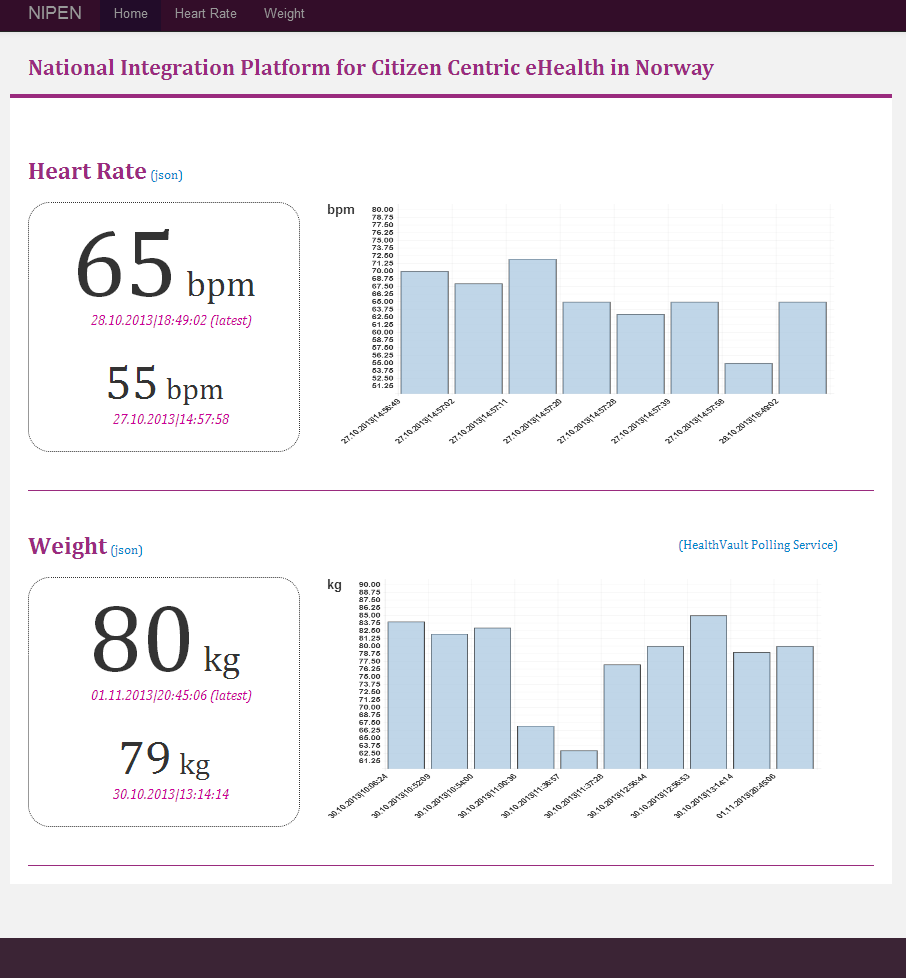
\includegraphics[scale=0.50]{../Figures/front-endfinal.png}
\includegraphics[scale=0.4]{../Figures/frontend-main-page.png}
\caption{Front-end final}
\label{figure:front-endfinal}
\end{figure}

\textbf{Functional requirements for the web front-end}

\begin{table}[H]
\begin{center}
\begin{tabular}{ | c | p{9cm} | c | c |}
  \hline
  ID & Description & Priority & Status\\
  \hline\noalign{\smallskip}\noalign{\smallskip}\hline
  FW1	& The web frontend shall display the data stored by the Integration Platform using charts.	& High & Completed \\
  FW2	& The web frontend shall use Helsenorge color palette                                       & Low & Completed \\
  \hline
\end{tabular}
\end{center}
\caption{Fulfillment of functional requirements for the web front-end}
\label{table:fulfillemntofwebfront-end}
\end{table}

\subsection{Fulfillment of functional requirements for the heart rate application}

This subsection describes the functional requirements for the heart rate application and its state after the project completion.
In figure \ref{figure:appfinal} the design and final version can be seen.
The app is very simple but functional. 
The goal of the app was to be able to, with the help of the camera, to capture the heart rate of people.
Then with the click of a button transmitt the data to NIPEN.


\begin{figure}[H]
\centering
\includegraphics[scale=0.20]{../Figures/appfinal.png}
\caption{Heart rate application final}
\label{figure:appfinal}
\end{figure}

\textbf{Fulfillment of functional requirements for Heart rate application}

\begin{table}[H]
\begin{center}
\begin{tabular}{ | c | p{9cm} | c | c |}
  \hline
  ID & Description & Priority & Status\\
  \hline\noalign{\smallskip}\noalign{\smallskip}\hline
  FHR1	& The application shall measure user’s heart rate using the device camera    & High & Completed \\
  FHR2	& The application shall display the last measurement on the screen.          & Med & Completed \\
  FHR3	& The application shall forward the data to the IP using its REST endpoint.  & High & Completed \\
  \hline
\end{tabular}
\end{center}
\caption{Fulfillment of functional requirements for the heart rate application}
\label{table:fulfillemntofapp}
\end{table}

\subsection{Fulfillment of functional requirements for Weight application}

This subsection describes the functional requirements for the weight application and its state after the project completion.
In figure \ref{figure:weightapp} the design and final version can be seen.
The goal of this app was to get weight data from Microsoft HealthVault and send it to NIPEN.

\begin{figure}[H]
\centering
\includegraphics[scale=0.20]{../Figures/weightappfinal.png}
\caption{Fulfillment of weight application}
\label{figure:weightappfinal}
\end{figure}

\textbf{Functional requirements for Weight application}

\begin{table}[H]
\begin{center}
\begin{tabular}{ | c | p{9cm} | c | c |}
  \hline
  ID & Description & Priority & Status\\
  \hline\noalign{\smallskip}\noalign{\smallskip}\hline
  FHV1	& The application shall fetch weight data from HealthVault.						      & High & Unkown \\
  FHV2	& The application shall show the user the data it has fetched.              & Med & Unkown \\
  FHV3	& The application shall forward the data to the IP using its REST endpoint. & High & Unkown \\
  \hline
\end{tabular}
\end{center}
\caption{Fulfillemnt of functional requirements for Weight application}
\label{table:fulfillemntweightapp}
\end{table}

\subsection{Fulfillment of non-funcional requirements}
This subsection describes the non-functional requirements and its state after the project completion. 

\begin{table}[H]
\begin{center}
\begin{tabular}{ | c | c |p{6.5cm} | c | c |}
  \hline
  ID & Category & Description & Priority & Status\\
  \hline\noalign{\smallskip}\noalign{\smallskip}\hline
  NF1 & Documentation & The system shall be thoroughly documented, both at the code level and by the document ‘project report’.
  & High & Completed \\
  NF2 & Documentation & Although security and privacy are not requirements for the product they are important topics to be discussed in the documentation.
  & High & Completed \\
  NF3 & Open-source	& The product shall be released under a permissive license approved by the product owner.
  & High & Completed \\
  NF4 & Interoperability & The system shall provide a good degree of interoperability. Third party application developers should be put in the condition to develop third party (interoperable) solutions rapidly.
  & High & Completed \\
  NF5 & Interoperability & A number of two-three prototype applications shall be developed in order to showcase the functionality of the system.
  & High & Completed \\
  NF6 & Accessibility & The web-frontend should have a good degree of accessibility. It should have a rather simple design and use a user-provided palette.
  & Low & Completed \\
  \hline
\end{tabular}
\end{center}
\caption{Fulfillment of non-functional requirements}
\label{table:fullfilmentnonfunctionalreq}
\end{table} 

\section{Further work}

Our NIPEN implementation and the belonging applications are mostly a proof of concept. 
The most important task of the client to do next will be to figure out if there is an interest in Helsenorge for this type of system.
The most important factor for this system is the value it delivers to the educated medical professionals. 
If this is something that gives the medical professionals additional value and makes it easier for them to understand the patiens health. 
A cost and benefit analysis of this system needs to be done to analyse the total value this system will give will be an important factor in deciding where to go next. 
The thought is that citizens can collect all types of health data and that even though their measurements might be imprecise that quantity of health data will overall improve the quality. 
This system is definitely possible to implement at a larger scale at a high cost.
The toughest part will be to convince the medical professionals to start using new methods and systems. 
Many will be pessimistic for this kind of system knowing that the data at some degree could not be dependent upon.
The important part to consider then is that even though specific data might be inaccurate it will be a lot easier to analyse trends and get a sense of the citizens habits. 

The value of this system can be hard to measure but already many people today do these kinds of measurements and the adaption is increasing. 
Earlier this year Pew Research Center’s Internet \& American Life Project released their findings of the role of Internet and technology in health and wellness. 
Their report, Tracking for Health can be found here http://pewinternet.org/Reports/2013/Tracking-for-Health.aspx, is focused on how people self-track.
In the research paper they found that 7 out of 10 adults track their health.
While 1 in 5 use technology to log this. 
What is important to note from the findings they did is that over half of those who keep a record of their health indicate that their tracking and recordkeeping has changed their approach to health.
The conclusion that can be taken from this is that the act of tracking alone affects the overall health and mindset of the citizen. 

\subsection{Third-party applications}

We developed three applications all interacting with our implementation of NIPEN. 
The idea behind making a portal like this is to open the API up to all developers so the NIP can be interoperable between all platforms, systems, applications and users. 
The ideal goal is to have a platform that reaches all types of users. 
The total cost of the project can be lowered by this because support for the system can be done by the developers of the different third-party applications. 
It is also possible for some developers to develop proxies for popular third-party applications.


\section{Summary}
In this chapter we have looked at what requirements our project have fulfilled. 
We have also discuessed what the next steps for pursuing the continues development of this platform. 

We are glad that we manage to implement most of the requirements meaning we made a realistic assumptions of what we could accomplish in the given time with the members we had. 
Although some of the syncronisation did not work ideeal it was not cause by our system but by third-party systems not working ideally. 
This project is an interesting idea and finding a way to unify the collection of health data of citizens will lead to a better understanding of citizen health and an easier overview of what can be improved for a better quality of life.  

\chapter{Reflection}
\lhead{Chapter 16. \emph{Reflection}}

\section{Suggestions for course improvements}
In all courses there are opportunities for improvement.
In this section we will discuss what we thought could be better, clearer and more efficient.

Firstly, we as a group felt that there was a lot of information we didn't get from the start. 
The first day of the course was the day we meet the client and our group members had not prepared for this.
The first couple of weeks there was a lack of information about what was expected and what was to be delivered.
We had to figure out a lot along the way.

This project would definitively improve with having more group members. 
We ended up being only three people while this project was really meant for atleast five people.
That left us with a lot of tasks and a lot of extra work to do.
Especially writing the report and developing the project would be a lot better with more members and work hours. 
We are pleased with the result of our project but it had potential to be a lot better with more hours of work which would only come from more group members. 

There were also some lectures throughout the semester. 
The times of these lectures were put at random times and not in the specified course time slots.
This lead to a lot of conflicts between course.
We advice that the course leaders try their best to plan lectures in the appointed timeslots so this won't happen in future years. 

We were early in reserving rooms for this course so we were maybe lucky in getting a room that we could work in this semester. 
Maybe other groups were not as lucky. 
The reserving of the rooms took some time for us to fix. 
It would be better for us to get a room appointed to our group that we could work in every week. 




\iffalse
Our NIPEN implementation and the belonging applications are mostly a proof of concept. 
The most important task of the client to do next will be to figure out if there is an interest in Helsenorge for this type of system.
The most important factor for this system is the value it delivers to the educated medical professionals. 
If this is something that gives the medical professionals additional value and makes it easier for them to understand the patients health. 
A cost and benefit analysis of this system needs to be done to analyse the total value this system will give will be an important factor in deciding where to go next.
The thought is that citizens can collect all types of health data and that even though their measurements might be imprecise that quantity of health data will overall improve the quality.
This system is definitely possible to implement at a larger scale at a high cost.
The toughest part will be to convince the medical professionals to start using new methods and systems. 
Many will be pessimistic for this kind of system knowing that the data at some degree could not be dependent upon.
The important part to consider then is that even though specific data might be inaccurate it will be a lot easier to analyse trends and get a sense of the citizens habits. 

The value of this system can be hard to measure but already many people today do these kinds of measurements and the adaption is increasing. 
Earlier this year Pew Research Center’s Internet \& American Life Project released their findings of the role of Internet and technology in health and wellness. 
Their report, Tracking for Health can be found here http://pewinternet.org/Reports/2013/Tracking-for-Health.aspx, is focused on how people self-track.
In the research paper they found that 7 out of 10 adults track their health.
While 1 in 5 use technology to log this. 
What is important to note from the findings they did is that over half of those who keep a record of their health indicate that their tracking and recordkeeping has changed their approach to health.
The conclusion that can be taken from this is that the act of tracking alone affects the overall health and mindset of the citizen. 

\subsection{Third-party applications}

We developed three applications all interacting with our implementation of NIPEN. 
The idea behind making a portal like this is to open the API up to all developers so the NIP can be interoperable between all platforms, systems, applications and users. 
The ideal goal is to have a platform that reaches all types of users. 
The total cost of the project can be lowered by this because support for the system can be done by the developers of the different third-party applications. 
It is also possible for some developers to develop proxies for popular third-party applications.


%%%%
We are glad we managed to implement every requirement 
meaning we made a realistic assumptions of what we could accomplish in the given time with the members we had.
%Although some of the syncronisation did not work ideeal it was not cause by our system but by third-party systems not working ideally. 
This project is an interesting idea and finding a way to unify the collection of health data of citizens will lead to a better understanding of citizen health and to an \iffalse easier\fi overview of what can be improved for a better quality of life. 
\fi 


%------------------------------
%	THESIS CONTENT - APPENDICES
%------------------------------
\addtocontents{toc}{\vspace{2em}}
\appendix

% Appendix A - Customer Assignment

\chapter{Assignment for Customer driven project} 

\label{AppendixA}
\lhead{Appendix A. \emph{Assignemnt}}

\textbf{Assignment for Customer driven project}

\textbf{Title:} 	National Integration Platform for Citizen Centric eHealth in Norway \\*
\textbf{Customer (Company):} 	The Directorate of Health, Department of the Health Portal\\*
\textbf{Address:}			Universitetsgata 2, Oslo \\


\textbf{Assignment text:} \\
\textit{Background} \\
The Directorate of Health has a national the task of digitalizing Norwegian healthcare, both by providing coordinated services for specialist healthcare (hospitals) and by providing digital services for citizens in general and patients specifically. 
Examples of such services are ePrescriptions, that is implemented on a national basis, the National Summare Care Record, that will go live in Trondheim in August 2013, and the citizen centric health portal  (helsenorge.no) that has been live since June 2011.

National eHealth projects are complex, long running and costly. There are obvious reasons for this. 
Among these are the complexity and criticality of healthcare, and the scale that national eHealth services represents. 

At the same time, the trends in technology development and consumer adaption of new technology continue to develop. 
Moderate prices and consumer friendly devices that monitor individuals’ health and wellness are increasingly becoming available in the market space. 
Combined with a continuous increase in digital competence in the population, they will influence citizens’ behavior and perspective on their own health situation in the future.

In addition to this, private providers develop great eHealth solutions with consumer and patient orientation. Medhelp.org and Healthvault.com are only two among many examples. 
Ambient assisted living has the potential of revolutionizing life for senior citizens with failing health.

The relevant question is: How can the substantial and long running eHealth projects of the government sector connect to and leverage the dynamics in the market and consumer behavior? 
The answer under investigation is the National Integration Platform (NIP) for Citizen Centric eHealth in Norway. 

\textit{Assignment} \\* 
The assignment is to plan, design and describe a NIP, and to develop a prototype.

The task such a platform should fulfil is to offer interoperability with third party solutions based on available application programmable interfaces (APIs).
All third party solution providers must adhere to specified and standardized rules regarding authentication, security model, messaging and privacy to interact with the NIP. 

The intention of such a platform is to enable the following:
\begin{itemize}
\item Citizens’ ability to publish information they produce from devices in their possession and third party software solutions, including smart phone and tablet apps, into the government run citizen centric health portal (helsenorge.no)
\item Citizens’ ability to fetch information about themselves from helsenorge.no to import it into third party software solutions of their own choosing
\end{itemize}

The assignment is to describe the architecture and major components of the NIP, how it will function on the “outside” regarding third party integration, and on the “inside” regarding integration with helsenorge.no.

It is also essential that the solution adhere to Norwegian privacy regulation and information security. 
Its requirements for integration should also encourage privacy by design within third party solutions.

The prototype should make use of one or more use cases to demonstrate how interaction is performed, how privacy and security concerns are managed and how the end user experience will be. \\


Contact details: 

Name:		Helge T. Blindheim\\
Mobile:		466 75 321\\
E-mail:		helgetb@helsedir.no

 % A Assignment 
\chapter{How to build the project}
\label{AppendixB}
\lhead{Appendix B. \emph{Build project}} 

\section{Database}

Before deploying the NIPEN system it is necessary to set up the database.
We are running a MySQL server on a ubuntu machine, the version we are using is \textit{5.5.32-0ubuntu0.13.04.1}.
After the MySQL server is installed the file \textit{database.sql} must be used to set up the database.
It contains all the database tables we are using in our project.
The project folder in \textit{nipen\textbackslash src\textbackslash main\textbackslash resources\textbackslash database}, contains a file called \textit{Spring-Datasource.xml}.
This file contains the database location, user and password.
This must be set up according to the configurations of the MySQL database.

\section{NIPEN and the front-end}

Our back-end and front-end is running on an Apache Tomcat Server 7.0.35, it can be downloaded from the following link: \href{http://tomcat.apache.org/download-70.cgi}{http://tomcat.apache.org/download-70.cgi}.
By default the manager page of tomcat can be found at the following URL $<$server address$>$/manager.
On that page it is possible to upload a WAR file on to the server.

To create a WAR file of NIPEN and the front-end, Java compiler and maven must be installed on the system.
The Java compiler version we are using is 1.7.0\_25.
We are using Maven 3.1.0, and it can be downloaded on the following page: \href{http://maven.apache.org/download.cgi}{http://maven.apache.org/download.cgi}.
When maven is installed and configured on the system, we can create a war file of the NIPEN project.
First we need to locate the \textit{pom.xml} file in the NIPEN folder.
After that we need to open a command line in that folder and run the command: \begin{verbatim}
mvn package
\end{verbatim}
This will create a target folder that contains the file \textit{nipen.war}.
When deploying this file on the tomcat server both the back-end (NIPEN) and the front-end (the web page) will be deployed on the server.

\section{HealthVault Integration Service}

This is deployed in the same way as NIPEN, except that this does not need a database.
Find the folder of the web service that contains the pom file, then run \textit{mvn package}.
The war file can then be uploaded on to the tomcat server.

\section{Android applications}

To install the android applications it is needed to copy the two apk files on to an android device.
One apk file for the heart rate application and one for the weight application.
The applications can then be installed on the android device through the default package installer on the phone.
However, since these applications are not downloaded from Google Play, a setting needs to be set on the phone to allow instalment of files from unknown sources.
This setting is usually found under application settings on the android device, and is called \textit{Unknown Sources}. % B How to build
\chapter{Templates}
\label{AppendixC} 
\lhead{Appendix C. \emph{Templates}}

\section{Weekly status report}

\begin{center}
Weekly status report \#X\\*
Week NN \\*
Dates 2013-MM-DD - 2013-MM-DD \\*
TDT4290 Customer Driven Project - Group 17
\end{center}

1. Work done

\begin{table}
\begin{center}
\begin{tabular}{ l | l | l }
  \hline
  Activity & Planned & Actual \\
  \hline\noalign{\smallskip}\noalign{\smallskip}\hline
  Studies & Number & Number \\
  Project management & Number & Number \\
  System developement & Number & Number \\
  Application development & Number & Number \\
  Database developement & Number & Number \\
  Testing & Number & Number \\
  Report & Number & Number \\
  \hline
\end{tabular}
\end{center}
\caption{Activity chart}
\label{table:activityChartStatusReport}
\end{table}

1.2 Meetings

2. Plan for next week

3. Milestones

4. Problems


\section{Agenda for advisor meeting}

\begin{center}
Agenda for advisor meeting \#X\\*
2013-MM-DD\\*
\end{center}

% This one is appearing on the top of the page while I want it in the agenda. Maybe change it away from a table? How do you tab the content?
\begin{table}
\begin{center}
\begin{tabular}{ l | l }
Time and Data & 2013-MM-DD HH:MM \\
Place & Room \\
Attendees & Full name \\
Referent & Full name \\
\end{tabular}
\end{center}
\caption{Activity chart}
\label{table:activityChartAdvisorAgenda}
\end{table}


1. Approval of agenda \\
2. Approval of minutes from last advisor meeting \\
3. Comments to last weeks minutes \\
4. Approval of the weekly report \\
4.1 Work done \\
4.1.2 Meetings \\
4.2 Plan for next week \\
4.3 Milestones \\
4.4 Problems \\
5. Other \\
6. For next meeting \\


\section{Minutes of advisor meeting}

\begin{center}
Advisor meeting X \\
2013-MM-DD \\
\end{center}

Time and Data 	2013-MM-DD HH:MM \\
Place 			Room \\
Attendees  		Full name of attendees \\
Referent 		Full name \\

1. Approval of agenda \\
2. Approval of minutes from last advisor meeting \\
3. Comments to last weeks minutes \\
4. Approval of the status report \\
4.1 Summerise status report \\
4.2 Work done in period \\
4.3 Work for next period \\
4.4 Problems in period \\
5. Other \\
6. For next meeting \\
 

\section{Agenda for customer meeting}

\begin{center}
Agenda for customer meeting \#X\\*
2013-MM-DD\\*
\end{center}

% This one is appearing on the top of the page while I want it in the agenda. Maybe change it away from a table? How do you tab the content?
\begin{table}
\begin{center}
\begin{tabular}{ l | l }
Time and Data & 2013-MM-DD HH:MM \\
Place & Room \\
Attendees & Full name \\
Referent & Full name \\
\end{tabular}
\end{center}
\caption{Activity chart}
\label{table:activityChartCustomerAgenda}
\end{table}


1. Approval of agenda \\
2. Approval of minutes from last customer meeting \\
3. Comments to last weeks minutes \\
4. Scenario \\
5. Decisions \\
6. Other \\
7. For next meeting \\


\section{Minutes of customer meeting}

Customer meeting X 
2013-MM-DD

Time and Data 	2013-MM-DD HH:MM
Place			ROOM
Attendees  		Full name of attendees
Referent  		Full name

1. Approval agenda
2. Approval minutes from last customer meeting
3. Comments to last weeks minutes
4. Scenario
5. Decisions
6. For next meeting

\section{Agenda for internal meeting}

\section{Minutes of internal meeting} % C Templates
\chapter{Advisor meeting documents}
\label{AppendixD}
\lhead{Appendix D. \emph{Advisor}}

\section{Weekly status report}

\subsection{Week 35}

\subsection{Week 36}

\subsection{Week 37}

\subsection{Week 38}

\subsection{Week 39}

\subsection{Week 40}

\subsection{Week 41}

\subsection{Week 42}

\subsection{Week 43}

\subsection{Week 44}

\subsection{Week 45}

\subsection{Week 46}

\subsection{Week 47}

\section{Agenda for advisor meeting}

\subsection{1}


\section{Minutes of advisor meeting}

1 % D Advisor 
\chapter{Customer meeting documents}
\label{AppendixE}
\lhead{Appendix E. \emph{Customer}}

\iffalse
\includepdf[pages={1},scale=.9]{../Customer_meetings/1.pdf}
\includepdf[pages={1,2},scale=.9]{../Customer_meetings/2.pdf}

\begin{center}
\includegraphics[scale=0.8]{../Customer_meetings/3.pdf}
\end{center}
\fi

%\iffalse
\section{Overview of customer meetings}

\begin{table}[h]
\begin{center}
\begin{tabular}{ l | l | l }
  \hline
  Weekday & Date & Meeting Number \\
  \hline\noalign{\smallskip}\noalign{\smallskip}\hline
  	Wednesday 	&	21.08.2013 & 1 \\
	Monday		&	26.08.2013 & 2 \\
	Monday		& 	02.09.2013 & 3 \\
	Monday 		&	09.09.2013 & 4 \\
	Monday 		&	16.09.2013 & 5 \\
	Monday 		&	23.09.2013 & 6 \\
	Friday 		&	29.09.2013 & 7 \\
	Monday 		&	30.09.2013 & 8 \\
	Monday 		&	07.10.2013 & 9 \\
	Monday 		&	14.10.2013 & 10 \\
	Monday 		&	21.10.2013 & 11 \\
	Monday 		&	28.10.2013 & 12 \\
	Monday 		&	04.11.2013 & 13 \\
	Monday 		&	11.11.2013 & 14 \\
	Monday 		&	18.11.2013 & 15 \\
  \hline
\end{tabular}
\end{center}
\caption{Customer meetings}
\label{table:customermeetings}
\end{table}

\section{Agenda for customer meeting}

\section{Minutes of customer meeting}
%\fi
 % E Customer
\chapter{Internal meeting notes}
\label{AppendixF}
\lhead{Appendix F. \emph{Internal}}


\section{Overview of internal meetings}

\begin{table}[h]
\begin{center}
\begin{tabular}{ l | l | l }
  \hline
  Weekday & Date & Meeting Number \\
  \hline\noalign{\smallskip}\noalign{\smallskip}\hline
  	Wednesday 	&	21.08.2013 & 1 \\
	Monday		&	26.08.2013 & 2 \\
	Monday		& 	02.09.2013 & 3 \\
	Monday 		&	09.09.2013 & 4 \\
	Monday 		&	16.09.2013 & 5 \\
	Monday 		&	23.09.2013 & 6 \\
	Friday 		&	29.09.2013 & 7 \\
	Monday 		&	30.09.2013 & 8 \\
	Monday 		&	07.10.2013 & 9 \\
	Monday 		&	14.10.2013 & 10 \\
	Monday 		&	21.10.2013 & 11 \\
	Monday 		&	28.10.2013 & 12 \\
	Monday 		&	04.11.2013 & 13 \\
	Monday 		&	11.11.2013 & 14 \\
	Monday 		&	18.11.2013 & 15 \\
  \hline
\end{tabular}
\end{center}
\caption{Internal meetings}
\label{table:internalmeetings}
\end{table}

\section{Agenda for internal meeting}

\section{Minutes of internal meeting} % F Internal

\addtocontents{toc}{\vspace{2em}}
\backmatter

%-----------------
%	BIBLIOGRAPHY
%-----------------
\label{Bibliography}
\lhead{\emph{Bibliography}} % Change the page header to say "Bibliography"
\bibliographystyle{unsrtnat} % Use the "unsrtnat" BibTeX style for formatting the Bibliography
\bibliography{Bibliography} % The references (bibliography) information are stored in the file named "Bibliography.bib"
\end{document}  